\documentclass[xcolor={x11names}]{beamer}

\usepackage{tikz}
\usepackage{pgfplots}
\pgfplotsset{compat=1.16}

\usepackage{colortbl}
\usetikzlibrary{positioning,plotmarks}

\usepackage{graphicx}
\usepackage{hyperref}
\usepackage{mathtools}
\usepackage{amssymb}
\usepackage{tcolorbox}
\usepackage{multirow}
\DeclareMathOperator*{\argmax}{arg\,max}
\usepackage{booktabs}

\usetikzlibrary{arrows.meta, positioning, patterns, calc, shapes, shapes.geometric, decorations.pathreplacing, quotes, backgrounds, fit}

% Theme settings
\usetheme{Madrid}
\usecolortheme{seahorse}
\setbeamertemplate{navigation symbols}{}

% Custom commands
\newcommand{\E}{\mathbb{E}}

\title{Auction Theory for Business}
\subtitle{Strategic Market Design and Applications}
\author{Strategic Insights}
\date{\today}

\begin{document}

\begin{frame}
  \titlepage
\end{frame}

\begin{frame}{Today's Agenda}
  \tableofcontents
\end{frame}



%===============================================
\part{Why Auctions Matter}
%===============================================

\begin{frame}{Why Should You Care About Auctions?}
\textbf{Auctions are everywhere in business}
\begin{itemize}
  \item Google Ads (\$200+ billion annually, billions of auctions daily)
  \item Government contracts and procurement
  \item Spectrum licenses (\$100+ billion raised)
  \item Real estate and property sales
  \item Online marketplaces (eBay, stock exchanges)
  \item Art, wine, and collectibles
\end{itemize}


\textbf{Key Business Questions}
\begin{itemize}
  \item Which auction format should I use?
  \item How do I maximize revenue?
  \item How should I bid when participating?
  \item How do I prevent manipulation?
\end{itemize}


\textit{Good market design isn't just theory—it's a competitive advantage.}
\end{frame}

\begin{frame}{The Stakes Are High}
\textbf{Global Impact} Trillions of dollars transacted via auctions annually


\textbf{Examples of Design Impact}
\begin{itemize}
  \item \textbf{UK spectrum auction (2000)} \$35 billion raised with careful design
  \item \textbf{Switzerland spectrum (2000)} Only \$20 million (poor competition)
  \item \textbf{New Zealand disaster} Student bid \$1 for spectrum, won due to no reserve price
  \item \textbf{California energy crisis (2000-01)} \$40+ billion in excess costs from poor design
\end{itemize}


\textbf{Key Lesson} Small design choices = massive financial impact
\end{frame}

\begin{frame}{The Fundamental Challenge}
\begin{center}
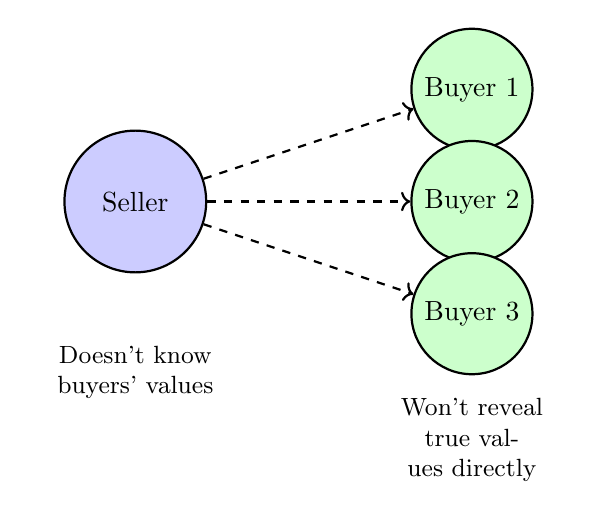
\begin{tikzpicture}[scale=0.95]
  % Seller
  \node[draw, thick, fill=blue!20, circle, minimum size=1.8cm] (seller) at (0,0) {Seller};
  
  % Buyers
  \node[draw, thick, fill=green!20, circle, minimum size=1.3cm] (b1) at (4.5,1.5) {Buyer 1};
  \node[draw, thick, fill=green!20, circle, minimum size=1.3cm] (b2) at (4.5,0) {Buyer 2};
  \node[draw, thick, fill=green!20, circle, minimum size=1.3cm] (b3) at (4.5,-1.5) {Buyer 3};
  
  % Arrows
  \draw[->, thick, dashed] (seller) -- (b1);
  \draw[->, thick, dashed] (seller) -- (b2);
  \draw[->, thick, dashed] (seller) -- (b3);
  
  % Labels
  \node[below, text width=2.5cm, align=center, font=\small] at (0,-1.8) {Doesn't know\\buyers' values};
  \node[below, text width=2.5cm, align=center, font=\small] at (4.5,-2.5) {Won't reveal\\true values directly};
\end{tikzpicture}
\end{center}


\textbf{Solution} Design an auction that reveals true values through competition
\end{frame}


\begin{frame}{Auction Theory Framework}
\begin{center}
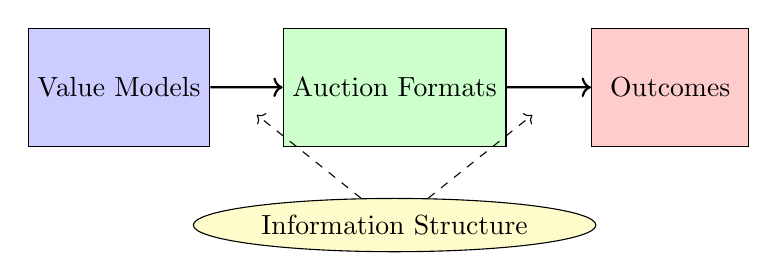
\begin{tikzpicture}[scale=0.7]
  % Main boxes
  \node[draw, rectangle, fill=blue!20, minimum width=2cm, minimum height=1.5cm] (values) at (0,3) {Value Models};
  \node[draw, rectangle, fill=green!20, minimum width=2cm, minimum height=1.5cm] (formats) at (5,3) {Auction Formats};
  \node[draw, rectangle, fill=red!20, minimum width=2cm, minimum height=1.5cm] (outcomes) at (10,3) {Outcomes};
  
  % Arrows
  \draw[->, thick] (values) -- (formats);
  \draw[->, thick] (formats) -- (outcomes);
  
  % Information flow
  \node[draw, ellipse, fill=yellow!20] (info) at (5,0.5) {Information Structure};
  \draw[->, dashed] (info) -- (2.5,2.5);
  \draw[->, dashed] (info) -- (7.5,2.5);
\end{tikzpicture}
\end{center}


\textbf{Key Questions in Auction Theory:}
\begin{itemize}
  \item How does information structure affect bidding?
  \item Which auction format maximizes revenue?
  \item When does the winner's curse arise?
  \item How can sellers use information strategically?
\end{itemize}
\end{frame}


\begin{frame}{The demand function}
\begin{center}
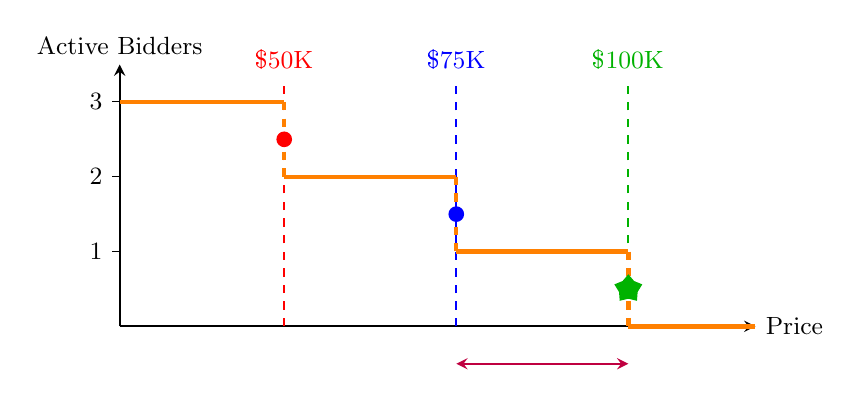
\begin{tikzpicture}[scale=0.95]
  % Set up axes
  \draw[thick, ->, >=stealth] (0,0) -- (8.5,0) node[right, font=\small] {Price};
  \draw[thick, ->, >=stealth] (0,0) -- (0,3.5) node[above, font=\small] {Active Bidders};
  
  % Y-axis labels
  \foreach \y/\label in {1/1, 2/2, 3/3} {
    \draw (0,\y) -- (-0.1,\y) node[left, font=\small] {\label};
  }
  
  % Valuations
  \draw[dashed, red, thick] (2.2,0) -- (2.2,3.3);
  \node[above, red, font=\small] at (2.2,3.3) {\$50K};
  
  \draw[dashed, blue, thick] (4.5,0) -- (4.5,3.3);
  \node[above, blue, font=\small] at (4.5,3.3) {\$75K};
  
  \draw[dashed, green!70!black, thick] (6.8,0) -- (6.8,3.3);
  \node[above, green!70!black, font=\small] at (6.8,3.3) {\$100K};
  
  % Step function
  \draw[ultra thick, orange] (0,3) -- (2.2,3);
  \draw[ultra thick, orange, dashed] (2.2,3) -- (2.2,2);
  \draw[ultra thick, orange] (2.2,2) -- (4.5,2);
  \draw[ultra thick, orange, dashed] (4.5,2) -- (4.5,1);
  \draw[ultra thick, orange] (4.5,1) -- (6.8,1);
  \draw[ultra thick, orange, dashed] (6.8,1) -- (6.8,0);
  \draw[ultra thick, orange] (6.8,0) -- (8.5,0);
  
  % Drop points
  \node[circle, fill=red, inner sep=2pt] at (2.2,2.5) {};
  \node[right, red, font=\small] at (2.4,2.5) {~};
  
  \node[circle, fill=blue, inner sep=2pt] at (4.5,1.5) {};
  \node[right, blue, font=\small] at (4.7,1.5) {};
  
  \node[star, star points=5, fill=green!70!black, inner sep=2.5pt] at (6.8,0.5) {};
  \node[right, green!70!black, font=\small] at (7.0,0.5) {};
  
  % Payment
  \draw[<->, >=stealth, thick, purple] (4.5,-0.5) -- (6.8,-0.5);
\end{tikzpicture}
\end{center}

\textbf{Insight 1} If mechanism $ \rightarrow p > v_2 \rightarrow  b_2 \ne v_ 2 $ \\
\textbf{Insight 2} Red arrow is efficient price area
\end{frame}

\part{prereq}

\section{Game-Theoretic Foundations}

\begin{frame}{Strategic Form Games}
\textbf{Definition:} A game $\Gamma = \langle N, (S_i)_{i \in N}, (u_i)_{i \in N} \rangle$ consists of:
\begin{itemize}
  \item \textbf{Players:} $N = \{1, 2, \ldots, n\}$
  \item \textbf{Strategy spaces:} $S_i$ for each player $i$
  \item \textbf{Payoff functions:} $u_i: S_1 \times \cdots \times S_n \to \mathbb{R}$
\end{itemize}


\textbf{Solution Concepts:}
\begin{enumerate}
  \item \textbf{Dominant Strategy:} $s_i^* \in S_i$ such that
  \[u_i(s_i^*, s_{-i}) \geq u_i(s_i, s_{-i}) \quad \forall s_i \in S_i, \forall s_{-i} \in S_{-i}\]
  
  \item \textbf{Nash Equilibrium:} Profile $(s_1^*, \ldots, s_n^*)$ where
  \[u_i(s_i^*, s_{-i}^*) \geq u_i(s_i, s_{-i}^*) \quad \forall s_i \in S_i, \forall i \in N\]
\end{enumerate}
\end{frame}

\begin{frame}{Incomplete Information Games}
\textbf{Harsanyi Transformation:}
\begin{itemize}
  \item Nature determines types $\theta = (\theta_1, \ldots, \theta_n)$
  \item Player $i$ observes only $\theta_i$
  \item Common prior: $\theta \sim F$ where $F$ is common knowledge
  \item Strategy: $s_i: \Theta_i \to S_i$
\end{itemize}


\textbf{Bayesian Nash Equilibrium:}

Strategy profile $(s_1^*, \ldots, s_n^*)$ where each $s_i^*: \Theta_i \to S_i$ satisfies:
\[s_i^*(\theta_i) \in \argmax_{s_i} \mathbb{E}_{\theta_{-i}|\theta_i}[u_i(s_i, s_{-i}^*(\theta_{-i}), \theta_i, \theta_{-i})]\]


\textbf{Key Insight:} Each type of each player best responds to beliefs about others' strategies
\end{frame}

%-------------------------------------------------
\section{Order Statistics Theory}

\begin{frame}{Order Statistics: Definition and Notation}
\textbf{Setup:} Given $n$ i.i.d. random variables $X_1, X_2, \ldots, X_n \sim F$


\textbf{Order Statistics:} Rearrange in ascending order
\[X_{(1)} \leq X_{(2)} \leq \cdots \leq X_{(n)}\]


\textbf{Alternative Notation (Auctions):} Often use descending order
\[v_{(1)} \geq v_{(2)} \geq \cdots \geq v_{(n)}\]
where $v_{(1)} = \max\{v_1, \ldots, v_n\}$ and $v_{(n)} = \min\{v_1, \ldots, v_n\}$


\textbf{Why Important for Auctions?}
\begin{itemize}
  \item Winner has highest valuation: $v_{(1)}$
  \item Second-price auctions: Winner pays $v_{(2)}$
  \item Revenue comparisons require $\mathbb{E}[v_{(1)}]$ and $\mathbb{E}[v_{(2)}]$
\end{itemize}
\end{frame}

\begin{frame}{Distribution of Order Statistics}
\textbf{CDF of $k$-th Order Statistic:}

The probability that the $k$-th smallest value is at most $x$:
\[G_{(k)}(x) = \Pr(X_{(k)} \leq x) = \sum_{j=k}^n \binom{n}{j} F(x)^j [1-F(x)]^{n-j}\]

\textbf{Intuition:} At least $k$ of the $n$ values must be $\leq x$


\textbf{PDF of $k$-th Order Statistic:}
\[g_{(k)}(x) = \frac{n!}{(k-1)!(n-k)!} F(x)^{k-1}[1-F(x)]^{n-k}f(x)\]

\textbf{Special Cases:}
\begin{itemize}
  \item Maximum: $G_{(n)}(x) = F(x)^n$, $g_{(n)}(x) = nF(x)^{n-1}f(x)$
  \item Minimum: $G_{(1)}(x) = 1-(1-F(x))^n$, $g_{(1)}(x) = n(1-F(x))^{n-1}f(x)$
\end{itemize}
\end{frame}

\begin{frame}{First and Second Order Statistics}
\textbf{First Order Statistic (Maximum):}
\begin{itemize}
  \item Distribution: $G_{(1)}(v) = F(v)^n$
  \item Density: $g_{(1)}(v) = nF(v)^{n-1}f(v)$
  \item Expected value: $\mathbb{E}[v_{(1)}] = \int_{\underline{v}}^{\bar{v}} v \cdot nF(v)^{n-1}f(v)dv$
\end{itemize}


\textbf{Second Order Statistic:}
\begin{itemize}
  \item Distribution: $G_{(2)}(v) = nF(v)^{n-1}[1-F(v)] + F(v)^n$
  \item Density: $g_{(2)}(v) = n(n-1)F(v)^{n-2}[1-F(v)]f(v)$
  \item Expected value: $\mathbb{E}[v_{(2)}] = \int_{\underline{v}}^{\bar{v}} v \cdot g_{(2)}(v)dv$
\end{itemize}

\textbf{Useful Identity:}
\[\mathbb{E}[v_{(2)}] = n\mathbb{E}[v_{(1,n-1)}] - (n-1)\mathbb{E}[v_{(1,n)}]\]
where $v_{(1,m)}$ denotes the maximum of $m$ draws
\end{frame}

\begin{frame}{Uniform Distribution: Key Results}
\textbf{For $U[0,1]$ distribution:}


\textbf{General Formula:}
\[\mathbb{E}[X_{(k)}] = \frac{k}{n+1}\]


\textbf{Intuition:} Order statistics divide $[0,1]$ into $n+1$ equal segments in expectation


\textbf{Examples:}
\begin{itemize}
  \item $n=2$: $\mathbb{E}[v_{(1)}] = \frac{2}{3}$, $\mathbb{E}[v_{(2)}] = \frac{1}{3}$
  \item $n=3$: $\mathbb{E}[v_{(1)}] = \frac{3}{4}$, $\mathbb{E}[v_{(2)}] = \frac{2}{4} = \frac{1}{2}$
  \item $n=10$: $\mathbb{E}[v_{(1)}] = \frac{10}{11}$, $\mathbb{E}[v_{(2)}] = \frac{9}{11}$
\end{itemize}

\textbf{Variance:}
\[\text{Var}(X_{(k)}) = \frac{k(n-k+1)}{(n+1)^2(n+2)}\]
\end{frame}

\begin{frame}{Order Statistics: Computational Examples}
\textbf{Example 1: Two Dice Rolls}
\begin{itemize}
  \item Roll two dice, let $V_{(1)} \geq V_{(2)}$ be the ordered outcomes
  \item Distribution of maximum:
  \begin{center}
  \begin{tabular}{c|cccccc}
  $v$ & 1 & 2 & 3 & 4 & 5 & 6 \\
  \hline
  $\Pr(V_{(1)} = v)$ & 1/36 & 3/36 & 5/36 & 7/36 & 9/36 & 11/36
  \end{tabular}
  \end{center}
  \item $\mathbb{E}[V_{(1)}] = 161/36 \approx 4.47$
  \item $\mathbb{E}[V_{(2)}] = 91/36 \approx 2.53$
\end{itemize}


\textbf{Example 2: Exponential Distribution}
\begin{itemize}
  \item If $X_i \sim \text{Exp}(\lambda)$ i.i.d., then:
  \item $X_{(1)} \sim \text{Exp}(n\lambda)$ (minimum is also exponential)
  \item $\mathbb{E}[X_{(1)}] = \frac{1}{n\lambda}$
\end{itemize}
\end{frame}

%-------------------------------------------------
\section{Information Structures}

\begin{frame}{Types of Information in Auctions}
\textbf{1. Independent Private Values (IPV):}
\begin{itemize}
  \item Each bidder knows own valuation exactly: $v_i$
  \item Values are private information, drawn i.i.d. from $F$
  \item Learning others' values doesn't change own value
  \item Example: Personal use items (used car, collectible)
\end{itemize}


\textbf{2. Common Values (CV):}
\begin{itemize}
  \item Single unknown value $V$ same for all bidders
  \item Each bidder receives private signal $s_i$ about $V$
  \item Winner's curse: Winning means you had highest estimate
  \item Example: Oil drilling rights, company takeovers
\end{itemize}


\textbf{3. Interdependent/Affiliated Values:}
\begin{itemize}
  \item General case: $v_i = v_i(s_1, \ldots, s_n)$
  \item Signals may be correlated (affiliated)
  \item Encompasses both IPV and CV as special cases
\end{itemize}
\end{frame}


\begin{frame}{Understanding Value Types}

\begin{block}{Private Values value is independent of others}
\begin{itemize}
  \item Personal consumption items
  \item Office space for your own use
  \item Company car for internal use
\end{itemize}
\end{block}

\begin{block}{Common Values value is the same for everyone}
\begin{itemize}
  \item Oil drilling rights (unknown amount of oil)
  \item Company acquisition (unknown future profits)
  \item Government bonds
\end{itemize}
\end{block}

\begin{block}{Mixed Values}
\begin{itemize}
  \item Real estate (personal use + investment value)
  \item Art (enjoyment + resale value)
\end{itemize}
\end{block}
\end{frame}


\begin{frame}{Visualization: Value Types Spectrum}
\begin{center}
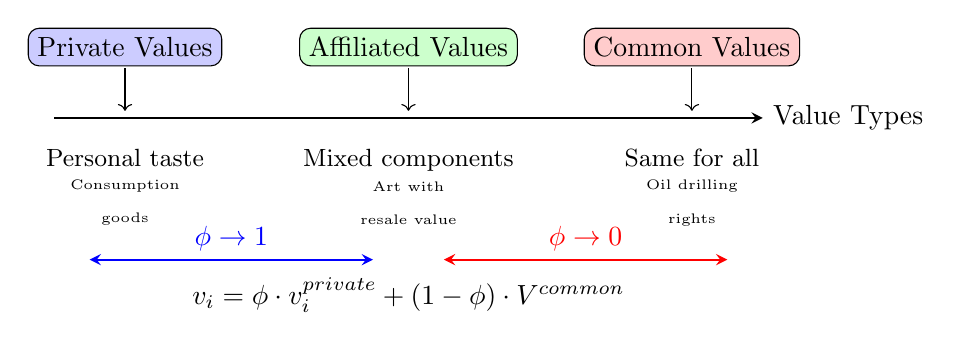
\begin{tikzpicture}[scale=0.9]
  % Spectrum line
  \draw[thick, ->, >=stealth] (0,0) -- (10,0) node[right] {Value Types};
  
  % Private Values
  \node[draw, fill=blue!20, rounded corners] at (1,1) {Private Values};
  \draw[->] (1,0.7) -- (1,0.1);
  \node[below] at (1,-0.3) {\small Personal taste};
  
  % Affiliated Values
  \node[draw, fill=green!20, rounded corners] at (5,1) {Affiliated Values};
  \draw[->] (5,0.7) -- (5,0.1);
  \node[below] at (5,-0.3) {\small Mixed components};
  
  % Common Values
  \node[draw, fill=red!20, rounded corners] at (9,1) {Common Values};
  \draw[->] (9,0.7) -- (9,0.1);
  \node[below] at (9,-0.3) {\small Same for all};
  
  % Examples
  \node[align=center] at (1,-1.2) {\tiny Consumption\\\tiny goods};
  \node[align=center] at (5,-1.2) {\tiny Art with\\\tiny resale value};
  \node[align=center] at (9,-1.2) {\tiny Oil drilling\\\tiny rights};
  
  % Formula
  \node at (5,-2.5) {$v_i = \phi \cdot v_i^{private} + (1-\phi) \cdot V^{common}$};
  \draw[<->, >=stealth, thick, blue] (0.5,-2) -- (4.5,-2);
  \node[blue] at (2.5,-1.7) {$\phi \to 1$};
  \draw[<->, >=stealth, thick, red] (5.5,-2) -- (9.5,-2);
  \node[red] at (7.5,-1.7) {$\phi \to 0$};
\end{tikzpicture}
\end{center}
\end{frame}



\begin{frame}{Common Knowledge and Beliefs}
\textbf{Common Knowledge:}

Event $E$ is common knowledge if:
\begin{enumerate}
  \item Everyone knows $E$
  \item Everyone knows that everyone knows $E$
  \item Everyone knows that everyone knows that everyone knows $E$
  \item ... (ad infinitum)
\end{enumerate}


\textbf{In Auctions, Common Knowledge Includes:}
\begin{itemize}
  \item Number of bidders $n$
  \item Auction format and rules
  \item Distribution $F$ (but not realizations)
  \item Rationality of all bidders
  \item Reserve price (if public)
\end{itemize}


\textbf{Private Information:}
\begin{itemize}
  \item Own valuation or signal
  \item Own bidding strategy (in sealed-bid)
  \item Others' valuations or signals
\end{itemize}
\end{frame}

%-------------------------------------------------
\section{Auction Formats}

\begin{frame}{Standard Auction Formats}
\textbf{Open Auctions:}
\begin{itemize}
  \item \textbf{English (Ascending):} Price rises, bidders drop out
  \item \textbf{Dutch (Descending):} Price falls, first to accept wins
\end{itemize}


\textbf{Sealed-Bid Auctions:}
\begin{itemize}
  \item \textbf{First-Price:} Highest bid wins, pays own bid
  \item \textbf{Second-Price (Vickrey):} Highest bid wins, pays second-highest bid
\end{itemize}


\textbf{Strategic Equivalences (IPV):}
\begin{itemize}
  \item Dutch $\equiv$ First-Price Sealed-Bid
  \item English $\approx$ Second-Price Sealed-Bid
\end{itemize}


\textbf{Dominant Strategies:}
\begin{itemize}
  \item Second-Price: Bid true value (truthful)
  \item English: Stay in until price exceeds value
  \item First-Price/Dutch: No dominant strategy (bid shading)
\end{itemize}
\end{frame}

%-------------------------------------------------
\section{Equilibrium Concepts}

\begin{frame}{Bayesian Nash Equilibrium in Auctions}
\textbf{Definition:} Strategy profile $\beta^* = (\beta_1^*, \ldots, \beta_n^*)$ is a BNE if:
\[\beta_i^*(v_i) \in \argmax_{b} \mathbb{E}_{v_{-i}}[u_i(b, \beta_{-i}^*(v_{-i}), v_i)]\]


\textbf{Symmetric Equilibrium:}
\begin{itemize}
  \item All bidders use same strategy: $\beta_i = \beta$ for all $i$
  \item Strategy is strictly increasing in valuation
  \item Boundary condition: $\beta(\underline{v}) = \underline{v}$ (or 0)
\end{itemize}


\textbf{First-Price Auction Equilibrium (IPV):}
\[\beta(v) = v - \frac{\int_{\underline{v}}^v F(t)^{n-1}dt}{F(v)^{n-1}}\]

\textbf{Uniform $[0,1]$ Case:}
\[\beta(v) = \frac{n-1}{n}v\]
\end{frame}

\begin{frame}{Revenue Equivalence Theorem}
\textbf{Theorem (Vickrey 1961, Riley-Samuelson 1981):}

Under IPV with risk-neutral bidders and symmetric equilibrium:
\begin{itemize}
  \item All standard auctions yield same expected revenue
  \item Expected revenue = $\mathbb{E}[v_{(2)}]$ (second-order statistic)
\end{itemize}


\textbf{Conditions for Revenue Equivalence:}
\begin{enumerate}
  \item Independent private values
  \item Risk neutrality
  \item Symmetric bidders
  \item Same allocation rule (efficient)
  \item Same payment by lowest type
\end{enumerate}


\textbf{Breaking Revenue Equivalence:}
\begin{itemize}
  \item Risk aversion $\Rightarrow$ First-price dominates
  \item Affiliated values $\Rightarrow$ English dominates
  \item Asymmetric bidders $\Rightarrow$ No general ranking
\end{itemize}
\end{frame}

%-------------------------------------------------
\section{Mathematical Tools and Techniques}

\begin{frame}{Differential Equations in Auction Theory}
\textbf{First-Order Approach:}

For symmetric equilibrium $\beta(v)$ in first-price auction:
\begin{enumerate}
  \item Bidder's problem: $\max_b (v-b) \cdot \Pr(\text{win with } b)$
  \item FOC at equilibrium: Leads to differential equation
  \item General form: $\beta'(v) = h(v)(v - \beta(v))$
  \item Boundary condition: $\beta(\underline{v}) = \underline{v}$ or reserve price
\end{enumerate}


\textbf{Solution Technique:}
\begin{itemize}
  \item Rewrite as: $d[\beta(v)H(v)] = v \cdot dH(v)$
  \item Integrate with boundary condition
  \item Verify second-order conditions
\end{itemize}


\textbf{Example - Uniform Distribution:}
\[\beta'(v) = \frac{(n-1)(v-\beta(v))}{v} \Rightarrow \beta(v) = \frac{n-1}{n}v\]
\end{frame}

\begin{frame}{Integration by Parts in Revenue Calculations}
\textbf{Expected Revenue Formula:}
\[\mathbb{E}[\text{Revenue}] = \int_{\underline{v}}^{\bar{v}} \beta(v) \cdot g_{(1)}(v)dv\]


\textbf{Key Technique:} Integration by parts
\begin{align*}
\int_{\underline{v}}^{\bar{v}} v \cdot dF^n(v) &= [v \cdot F^n(v)]_{\underline{v}}^{\bar{v}} - \int_{\underline{v}}^{\bar{v}} F^n(v)dv\\
&= \bar{v} - \int_{\underline{v}}^{\bar{v}} F^n(v)dv
\end{align*}


\textbf{Useful Identity for Second-Order Statistic:}
\[\mathbb{E}[v_{(2)}] = \int_{\underline{v}}^{\bar{v}} v \cdot n(n-1)F^{n-2}(1-F)f \, dv\]

\textbf{Revenue Equivalence Check:}
All standard auctions yield $\mathbb{E}[\text{Revenue}] = \mathbb{E}[v_{(2)}]$
\end{frame}

%-------------------------------------------------
\section{Extensions and Applications}

\begin{frame}{Reserve Prices and Optimal Auctions}
\textbf{Optimal Reserve Price:}

Maximizes expected revenue subject to participation constraints


\textbf{Myerson (1981) Result:}
\[r^* = v_s + \frac{1-F(r^*)}{f(r^*)}\]
where $v_s$ is seller's valuation


\textbf{Virtual Valuation:}
\[\psi(v) = v - \frac{1-F(v)}{f(v)}\]

\begin{itemize}
  \item Optimal auction allocates to bidder with highest positive virtual valuation
  \item Reserve price where $\psi(r^*) = 0$
\end{itemize}


\textbf{Example - Uniform $[0,1]$:}
\begin{itemize}
  \item Virtual valuation: $\psi(v) = 2v - 1$
  \item Optimal reserve: $r^* = 1/2$
  \item Independent of number of bidders!
\end{itemize}
\end{frame}

\begin{frame}{All-Pay Auctions and Contests}
\textbf{All-Pay Auction:}
\begin{itemize}
  \item Everyone pays their bid, only highest wins prize
  \item Models: R\&D races, political lobbying, litigation
\end{itemize}


\textbf{Equilibrium Bidding (Symmetric IPV):}
\[\beta_{AP}(v) = \int_{\underline{v}}^v t \cdot dF^{n-1}(t) = \mathbb{E}[v_{(1,n-1)}|v_{(1,n-1)} < v]\]


\textbf{Uniform $[0,1]$ Case:}
\[\beta_{AP}(v) = \frac{n-1}{n}v^n\]

\textbf{Revenue:}
\begin{itemize}
  \item Total revenue = $n \cdot \mathbb{E}[\beta_{AP}(v)]$ (all pay)
  \item Still equals $\mathbb{E}[v_{(2)}]$ under revenue equivalence!
\end{itemize}
\end{frame}

\begin{frame}{Common Values and Winner's Curse}
\textbf{Winner's Curse:}
\begin{itemize}
  \item In CV auctions, winning is ``bad news'' about value
  \item Winner had most optimistic signal
  \item Naive bidding leads to losses
\end{itemize}


\textbf{Equilibrium Adjustment:}

Rational bidders account for adverse selection:
\[\beta(s_i) = \mathbb{E}[V | s_i, \text{Win}] < \mathbb{E}[V | s_i]\]


\textbf{Mineral Rights Model:}
\begin{itemize}
  \item True value: $V = \frac{1}{n}\sum_{i=1}^n s_i$
  \item Signals: $s_i = V + \epsilon_i$, $\epsilon_i$ i.i.d.
  \item More bidders $\Rightarrow$ Worse winner's curse
  \item English auction reveals information, reduces curse
\end{itemize}

\textbf{Linkage Principle:}
More information revelation increases expected revenue
\end{frame}

%--------

%%%%%%%%%%%%%%%%%%%%%%%%
%%%%%%%%%%%%
%-------------------------------------------------
\section{Game Theory Preliminaries}

\begin{frame}{What Are We Studying? The Auction Game}
\textbf{The Basic Auction Story:}
\begin{itemize}
  \item Multiple people want the same thing (a house, a painting, ad space)
  \item Only one can have it (or limited quantities available)
  \item How do we decide who gets it and at what price?
\end{itemize}

\textbf{Why Game Theory?}
\begin{itemize}
  \item Your best strategy depends on what others do
  \item Others' strategies depend on what you do
  \item Everyone is trying to outsmart everyone else
  \item Information is often incomplete or asymmetric
\end{itemize}

\textbf{The Central Questions:}
\begin{itemize}
  \item How should rational bidders behave?
  \item What auction format maximizes seller revenue?
  \item How does information structure affect outcomes?
  \item When do auctions fail to work well?
\end{itemize}

\textit{Think of auctions as strategic battlegrounds where information, timing, and psychology all matter!}
\end{frame}

\begin{frame}{Game-Theoretic Foundations}
\textbf{Strategic Form Game:} $G = (N, (S_i)_{i \in N}, (u_i)_{i \in N})$
\begin{itemize}
  \item Players: $N = \{1, 2, \ldots, n\}$
  \item Strategy spaces: $S_i$ for player $i$
  \item Payoff functions: $u_i: S_1 \times \cdots \times S_n \to \mathbb{R}$
\end{itemize}

\textbf{Solution Concepts Hierarchy:}
\begin{center}
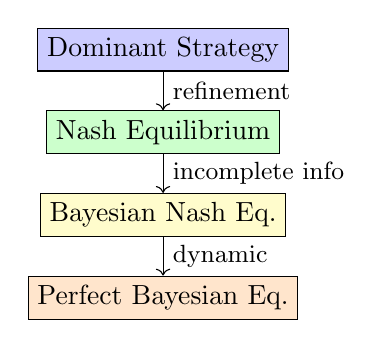
\begin{tikzpicture}[scale=0.7]
  \node[draw, rectangle, fill=blue!20] (dom) at (0,0) {Dominant Strategy};
  \node[draw, rectangle, fill=green!20] (ne) at (0,-1.5) {Nash Equilibrium};
  \node[draw, rectangle, fill=yellow!20] (bne) at (0,-3) {Bayesian Nash Eq.};
  \node[draw, rectangle, fill=orange!20] (pbe) at (0,-4.5) {Perfect Bayesian Eq.};
  
  \draw[->] (dom) -- (ne) node[midway, right] {\small refinement};
  \draw[->] (ne) -- (bne) node[midway, right] {\small incomplete info};
  \draw[->] (bne) -- (pbe) node[midway, right] {\small dynamic};
\end{tikzpicture}
\end{center}
\end{frame}

\begin{frame}{Order Statistics: Essential Theory}
\textbf{Definition:} For i.i.d. $X_1, \ldots, X_n \sim F$, order statistics are:
\[X_{(1)} \leq X_{(2)} \leq \cdots \leq X_{(n)}\]

\textbf{Distribution of $k$-th Order Statistic:}
\[F_{(k)}(x) = \sum_{j=k}^n \binom{n}{j} F(x)^j [1-F(x)]^{n-j}\]
\[f_{(k)}(x) = \frac{n!}{(k-1)!(n-k)!} F(x)^{k-1}[1-F(x)]^{n-k}f(x)\]

\begin{tcolorbox}[colback=blue!5!white,colframe=blue!75!black,title=Key Result for Auctions]
For uniform $[0,1]$ distribution:
\[\E[X_{(k)}] = \frac{k}{n+1}, \quad \text{Var}(X_{(k)}) = \frac{k(n-k+1)}{(n+1)^2(n+2)}\]
\end{tcolorbox}
\end{frame}

\begin{frame}{Game Theory Takeaways}
\textbf{What We Learned:}
\begin{itemize}
  \item \textbf{Strategic Thinking:} In auctions, you must think about what others are thinking
  \item \textbf{Solution Concepts:} Different levels of rationality lead to different predictions
  \item \textbf{Order Statistics:} The mathematics of "who has the highest value" is crucial
\end{itemize}

\textbf{Key Insights:}
\begin{itemize}
  \item Dominant strategies (like truthful bidding in second-price) are rare but powerful
  \item Most auction analysis requires equilibrium thinking
  \item The second-highest value matters as much as the highest!
\end{itemize}

\textbf{Why This Matters:}
\begin{itemize}
  \item Foundation for understanding bidding strategies
  \item Explains why different auction formats exist
  \item Shows how information and beliefs drive behavior
\end{itemize}
\end{frame}

%-------------------------------------------------
\section{Epistemic Foundations and Knowledge Operators}

\begin{frame}{Why Knowledge Matters in Auctions}
\textbf{The Information Puzzle:}
\begin{itemize}
  \item In auctions, what you know matters
  \item But what you know that others know also matters
  \item And what you know that others know that you know...
  \item This infinite regress is crucial for strategic reasoning!
\end{itemize}

\textbf{Common Knowledge in Practice:}
\begin{itemize}
  \item Auction rules must be common knowledge
  \item Reserve prices are often announced publicly (why?)
  \item Some information is deliberately kept private
  \item Strategic information revelation can increase revenue
\end{itemize}

\textit{Knowledge isn't just about facts—it's about knowing what others know!}
\end{frame}

\begin{frame}{Knowledge Operators: Philosophical Foundations}
\textbf{Epistemic Logic Framework:}
\begin{itemize}
  \item Knowledge operator $K_i$: ``agent $i$ knows that...''
  \item $K_i \varphi$ means ``agent $i$ knows proposition $\varphi$''
\end{itemize}

\textbf{S5 Axiom System (Kripke, 1963):}
\begin{enumerate}
  \item \textbf{Knowledge:} $K_i \varphi \rightarrow \varphi$ (truth axiom)
  \item \textbf{Positive Introspection:} $K_i \varphi \rightarrow K_i K_i \varphi$
  \item \textbf{Negative Introspection:} $\neg K_i \varphi \rightarrow K_i \neg K_i \varphi$
  \item \textbf{Distribution:} $K_i(\varphi \rightarrow \psi) \rightarrow (K_i \varphi \rightarrow K_i \psi)$
  \item \textbf{Necessitation:} If $\vdash \varphi$, then $\vdash K_i \varphi$
\end{enumerate}

\textbf{Philosophical Implications:}
\begin{itemize}
  \item Agents have perfect knowledge of their own knowledge state
  \item No false beliefs (knowledge implies truth)
  \item Logical omniscience problem: agents know all tautologies
\end{itemize}
\end{frame}

\begin{frame}{Kripke Structures and Possible Worlds}
\textbf{Formal Model:}
\begin{itemize}
  \item State space $\Omega$ (possible worlds)
  \item Accessibility relation $\sim_i \subseteq \Omega \times \Omega$ for each agent $i$
  \item Valuation function $V: \Omega \times \Phi \to \{0,1\}$
\end{itemize}

\textbf{Knowledge Definition:}
\[
(\Omega, \omega) \models K_i \varphi \iff \forall \omega' \in \Omega: \omega \sim_i \omega' \implies (\Omega, \omega') \models \varphi
\]

\textbf{Properties of $\sim_i$ in S5:}
\begin{itemize}
  \item \textbf{Reflexive:} $\omega \sim_i \omega$ (truth axiom)
  \item \textbf{Symmetric:} $\omega \sim_i \omega' \implies \omega' \sim_i \omega$
  \item \textbf{Transitive:} $\omega \sim_i \omega' \land \omega' \sim_i \omega'' \implies \omega \sim_i \omega''$
\end{itemize}

Therefore, $\sim_i$ forms an equivalence relation (information partition)
\end{frame}

\begin{frame}{Iterative Common Knowledge and Aumann(1976)}
\begin{align*}
E^1(\varphi) &= \bigwedge_{i \in N} K_i \varphi \quad \text{(everyone knows)} \\
E^k(\varphi) &= E(E^{k-1}(\varphi)) \quad \text{(k-th level mutual knowledge)} \\
C(\varphi) &= \bigwedge_{k=1}^{\infty} E^k(\varphi) \quad \text{(common knowledge)} \\
C(\varphi) &\leftrightarrow E(\varphi \land C(\varphi)) \quad \text{(Fixed Point)}
\end{align*}

\begin{center}
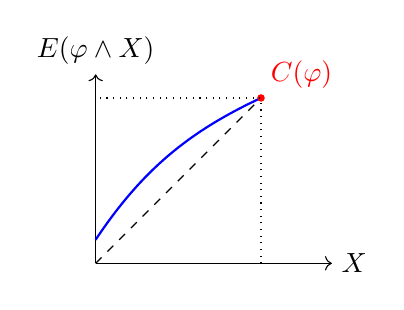
\begin{tikzpicture}[scale=0.6]
  \draw[->] (0,0) -- (5,0) node[right] {$X$};
  \draw[->] (0,0) -- (0,4) node[above] {$E(\varphi \land X)$};
  \draw[dashed] (0,0) -- (3.5,3.5);
  \draw[thick, blue] (0,0.5) .. controls (1,2) and (2,2.8) .. (3.5,3.5);
  \fill[red] (3.5,3.5) circle (0.08) node[above right] {$C(\varphi)$};
  \draw[dotted] (3.5,0) -- (3.5,3.5) -- (0,3.5);
\end{tikzpicture}
\end{center}
\end{frame}

\begin{frame}{The Coordinated Attack Problem}
\textbf{Byzantine Generals Paradox (Philosophical Insight):}
\begin{itemize}
  \item Two generals must coordinate attack
  \item Messages may be lost
  \item Common knowledge impossible with unreliable communication
\end{itemize}

\textbf{Formal Result:}
\begin{theorem}
In a system with possible communication failure, common knowledge of any non-trivial fact cannot be achieved in finite time.
\end{theorem}

\textbf{Auction Theory Implication:}
\begin{itemize}
  \item Perfect common knowledge is idealization
  \item Approximate common knowledge: $\varepsilon$-common belief
  \item Robust mechanism design accounts for higher-order uncertainty
\end{itemize}
\end{frame}

\begin{frame}{Knowledge and Information: Key Lessons}
\textbf{What We Learned:}
\begin{itemize}
  \item \textbf{Knowledge Hierarchy:} "I know" vs "We all know that we all know"
  \item \textbf{Common Knowledge:} The infinite mutual knowledge that enables coordination
  \item \textbf{Practical Limits:} Perfect common knowledge is impossible in real markets
\end{itemize}

\textbf{Real-World Applications:}
\begin{itemize}
  \item eBay shows bid history (creates common knowledge)
  \item Art auctions use elaborate signaling systems
  \item Financial markets have designated information releases
\end{itemize}

\textit{Remember: In auctions, it's not just what you know—it's what everyone knows that everyone knows!}
\end{frame}

%-------------------------------------------------
\section{Information Structure and Game-Theoretic Setup}

\begin{frame}{Understanding Information in Auctions}

\textbf{Private Values Example - Used Car:}
\begin{itemize}
  \item You know how much you need a car for commuting
  \item Others' valuations don't change your needs
  \item Your value is certain and private
\end{itemize}

\textbf{Common Values Example - Oil Drilling Rights:}
\begin{itemize}
  \item Nobody knows exactly how much oil is there
  \item Everyone gets different geological surveys (signals)
  \item The actual amount of oil is the same for everyone
  \item Learning others' signals would change your estimate
\end{itemize}

\textit{The information structure determines everything: bidding strategies, revenue, efficiency, and even whether the auction works at all!}
\end{frame}

\begin{frame}{Type Spaces and Beliefs}
\textbf{Harsanyi Type Space $(T_i, \tau_i, p_i)_{i \in N}$:}
\begin{itemize}
  \item $T_i$: Type space for player $i$
  \item $\tau_i: \Theta \to T_i$: Type function mapping states to types
  \item $p_i: T_i \to \Delta(T_{-i} \times \Theta)$: Belief function
\end{itemize}

\textbf{Consistency Requirements:}
\begin{enumerate}
  \item \textbf{Own-type awareness:} $p_i(t_i)(\{t_{-i}\} \times \{\theta\}) > 0 \implies \tau_i(\theta) = t_i$
  \item \textbf{Common prior (optional):} $\exists \mu \in \Delta(\Theta)$ such that beliefs derive from Bayesian updating
\end{enumerate}

\textbf{Universal Type Space (Mertens-Zamir, 1985):}
\begin{itemize}
  \item Contains all possible belief hierarchies
  \item $T_i^* = \prod_{k=1}^{\infty} \Delta^k$ where $\Delta^k$ is $k$-th order beliefs
  \item Every finite type space embeds into universal space
\end{itemize}
\end{frame}

\begin{frame}{Information Structures in Auctions}
\textbf{Private Values Model (PV):}
\begin{itemize}
  \item Value: $v_i = \theta_i$ (private information = value)
  \item Type space: $T_i = [\underline{v}, \overline{v}]$
  \item Common prior: $v_i \sim F$ i.i.d.
  \item Utility: $u_i(x, p, v_i) = v_i \cdot x_i - p_i$
\end{itemize}

\textbf{Common Values Model (CV):}
\begin{itemize}
  \item True value: $V(\theta)$ where $\theta = (s_1, \ldots, s_n)$
  \item Signal: $s_i \in S_i$ privately observed
  \item Value function: Often $V = \frac{1}{n}\sum_{i=1}^n s_i$ or $V = \max_i s_i$
  \item Utility: $u_i(x, p, \theta) = V(\theta) \cdot x_i - p_i$
\end{itemize}

\textbf{Interdependent Values (IV):}
\begin{itemize}
  \item General case: $v_i(s_1, \ldots, s_n)$
  \item Nests PV ($v_i(s) = s_i$) and CV ($v_i(s) = V(s) \, \forall i$)
  \item Single Crossing: $\frac{\partial^2 v_i}{\partial s_i \partial s_j} \geq 0$ (affiliation)
\end{itemize}
\end{frame}


\part{Definitions}

% %===============================================
\section{Standard Auction Formats}
%===============================================

\begin{frame}{Six auction Formats}
Let $v$ = your valuation, $b$ = your bid, $b_1$ = highest bid, $b_2$ = second-highest bid

\begin{enumerate}
  \item \textbf{English Auction (Ascending Price)}
  \item \textbf{Dutch Auction (Descending Price)}
  
  \item \textbf{Sealed-Bid First-Price}
  \begin{itemize}
    \item[] $\pi = \mathbb{P}(b = b_1) \cdot (v - b)$
  \end{itemize}
  
  \item \textbf{Sealed-Bid Second-Price (Vickrey)}
  \begin{itemize}
    \item[] $\pi = \mathbb{P}(b = b_1) \cdot (v - b_2)$
  \end{itemize}
  
  \item \textbf{All-Pay First Price}
  \begin{itemize}
    \item[] $\pi = \mathbb{P}(b = b_1) \cdot v - b$
  \end{itemize}
  
  \item \textbf{All-Pay Second Price (War of Attrition)}
  \begin{itemize}
    \item[] $\pi = \mathbb{P}(b = b_1) \cdot (v - b_2) - \mathbb{P}(b \neq b_1) \cdot b$
  \end{itemize}
\end{enumerate}

\end{frame}

\subsection{English Auction}

\begin{frame}{What is an English Auction?}

\begin{block}{Definition}
An \textbf{English auction} is a market mechanism where bidders \textbf{sequentially} indicate their interest in purchasing a product at a current price. Only the winner pays.
\end{block}

\begin{columns}[T]
\column{0.48\textwidth}
\begin{exampleblock}{Standard Ascending Format}
\begin{itemize}
\item Prices \textbf{increase} incrementally
\item Bidders signal their interest
\item Ends when only one bidder signals
\end{itemize}
\end{exampleblock}

\column{0.48\textwidth}
\begin{exampleblock}{Reverse English Format}
\begin{itemize}
\item Prices \textbf{decrease} incrementally
\item Bidders signal interest
\item Ends when only one bidder signals
\end{itemize}
\end{exampleblock}
\end{columns}

\begin{alertblock}{Note}
English = Ascending; \textbf{Reverse} Ascending = \textbf{Reverse} English
The terminology refers to the auction format, not the price direction.
\end{alertblock}

\end{frame}

\begin{frame}{English Auction: Equilibrium Analysis}
\textbf{Dominant Strategy:}
\begin{itemize}
  \item Stay in auction while price $p < v_i$
  \item Drop out when price $p \geq v_i$
  \item Strategy independent of beliefs about others
\end{itemize}


\textbf{Equilibrium Outcome:}
\begin{itemize}
  \item Bidder 2 drops out at $p = v_{(2)}$
  \item Bidder 1 (highest value) wins
  \item Pays price $p = v_{(2)}$ (second-highest valuation)
  \item Winner's surplus: $v_{(1)} - v_{(2)} > 0$
\end{itemize}


\textbf{Properties:}
\begin{itemize}
  \item \textcolor{green}{Pareto efficient (highest value wins)}
  \item Monopolist cannot extract full surplus
  \item Simple strategy (no need to know $F$ or $n$)
  \item Transparent process
\end{itemize}
\end{frame}


\begin{frame}{Derivation: English Auction}

\textbf{Claim:} Staying active while $p < v_i$ is weakly dominant

\textbf{Proof:}
Consider bidder $i$ with value $v_i$, current price $p$

\textbf{Case 1:} $p < v_i$
\begin{itemize}
  \item Stay active: Win if others drop first, payoff $= v_i - p_{final} \geq v_i - p > 0$
  \item Drop out: Lose, payoff $= 0$
  \item Staying dominates dropping
\end{itemize}

\textbf{Case 2:} $p \geq v_i$
\begin{itemize}
  \item Stay active: If win, pay $p \geq v_i$, payoff $\leq 0$
  \item Drop out: Lose, payoff $= 0$
  \item Dropping (weakly) dominates staying
\end{itemize}

\textbf{Equilibrium Bidding Function:}
$$b(v_i) = v_i \text{ (stay active until price reaches } v_i\text{)}$$

\textbf{Winner pays:} $p^* = v_{(2)}$ (second-highest valuation)
\end{frame}

\subsection{Dutch Auction}

\begin{frame}{What is a Dutch Auction?}
\begin{block}{Definition}
A \textbf{Dutch auction} is a market mechanism where an auctioneer \textbf{sequentially} changes the price until the first person signals their interest. The first bidder to accept, wins.
\end{block}
\begin{columns}[T]
\column{0.48\textwidth}
\begin{exampleblock}{Standard Descending Format}
\begin{itemize}
\item Prices \textbf{decrease} incrementally
\item Bidders watch and wait
\item First to accept the price wins
\end{itemize}
\end{exampleblock}
\column{0.48\textwidth}
\begin{exampleblock}{Reverse Dutch}
\begin{itemize}
\item Prices \textbf{increase} incrementally
\item Bidders watch and wait
\item First to accept the price wins
\end{itemize}
\end{exampleblock}
\end{columns}
\begin{alertblock}{Note}
\textbf{Reverse} Descending = \textbf{Reverse} Dutch; Descending = Dutch \\
The terminology refers to the auction format, not the price direction.
\end{alertblock}
\end{frame}


\begin{frame}{Dutch Auction: Strategic Equivalence}
\textbf{Claim:} Dutch and First-Price auctions are strategically equivalent

\textbf{Dutch Auction Decision:}
\begin{itemize}
  \item Choose stopping price $b$ before auction starts
  \item Accept when clock reaches $b$
  \item If someone else accepts first, lose
\end{itemize}

\textbf{First-Price Decision:}
\begin{itemize}
  \item Choose bid $b$ to submit in sealed envelope
  \item If $b$ is highest, win and pay $b$
  \item Otherwise lose
\end{itemize}

\textbf{Why Equivalent?}
\begin{itemize}
  \item Same information at decision time (only own value)
  \item Same action space (choose a price)
  \item Same payoff structure
  \item Same equilibrium strategies
\end{itemize}
\end{frame}


\begin{frame}{Derivation: Dutch Auction}
\textbf{Setup:}
\begin{itemize}
  \item Clock starts at high price, descends continuously
  \item First bidder to accept wins at current price
\end{itemize}

\textbf{Strategic Equivalence to First-Price:}

\textbf{Dutch Decision:} Choose stopping price $b$ ex-ante
\begin{itemize}
  \item Accept when clock reaches $b$
  \item Win if no one accepts earlier (i.e., $b > b_j$ for all $j \neq i$)
  \item Pay $b$ if win
  \item Payoff: $(v_i - b) \cdot \mathbb{P}(b > \max_{j \neq i} b_j)$
\end{itemize}

\textbf{First-Price Decision:} Submit sealed bid $b$
\begin{itemize}
  \item Win if $b > b_j$ for all $j \neq i$
  \item Pay $b$ if win
  \item Payoff: $(v_i - b) \cdot \mathbb{P}(b > \max_{j \neq i} b_j)$
\end{itemize}

\textbf{Conclusion:} Identical payoff structures $\Rightarrow$ identical equilibrium strategies

$$b_{Dutch}(v_i) = b_{First}(v_i) = \mathbb{E}[v_{(2)} \mid v_{(1)} = v_i]$$
\end{frame}

\subsection{Sealed-Bid First price}

\begin{frame}{What is a First Price Auction?}
\begin{block}{Definition}
A \textbf{first price auction} is a \textbf{simultaneous} market mechanism where the highest bidder wins and pays their own bid. 
\end{block}

\begin{exampleblock}{Sealed-Bid First Price Format}
\begin{itemize}
\item Bidders submit sealed bids
\item Highest bid wins the item
\item Winner pays their own bid
\end{itemize}
\end{exampleblock}

\begin{alertblock}{Note}
In a first price auction, bidders face a trade-off bidding high increases the chance of winning but decreases profit if they win. This is known as the bid-shading problem.
\end{alertblock}
\end{frame}


\begin{frame}{Sealed-Bid First price The Strategic Challenge}
\begin{center}
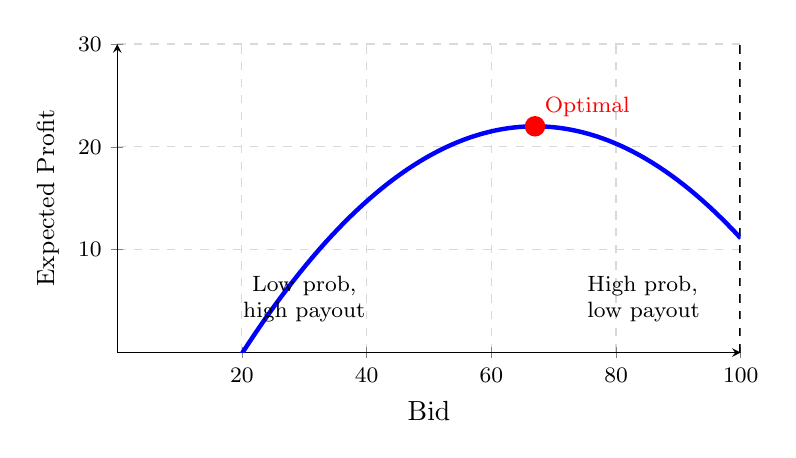
\begin{tikzpicture}[scale=1]
  \begin{axis}[
    xlabel={Bid},
    ylabel={Expected Profit},
    xmin=0, xmax=100,
    ymin=0, ymax=30,
    axis lines=middle,
    width=9.5cm,
    height=5.5cm,
    grid=major,
    grid style={dashed, gray!30},
    xtick={0,20,40,60,80,100},
    ytick={0,10,20,30},
    xlabel style={font=\small},
    xlabel near ticks, 
    ylabel near ticks, 
    ylabel style={font=\small},
    tick label style={font=\footnotesize}
  ]
  
  % True value line
  \addplot[domain=0:100, samples=2, very thick, black, dashed] coordinates {(100,0) (100,30)};
  \node[font=\footnotesize] at (axis cs:100,32) {Your Value \$100K};
  
  % Expected profit curve
  \addplot[domain=0:100, samples=100, ultra thick, blue] {-0.01*(x-67)^2 + 22};
  
  % Optimal bid marker
  \addplot[mark=*, mark size=3.5pt, only marks, red] coordinates {(67,22)};
  \node[above right, red, font=\footnotesize] at (axis cs:67,22) {Optimal};
  
  % Annotations
  \node[above, align=center, font=\footnotesize] at (axis cs:30,2) {Low prob, \\high payout};
  \node[above left, align=left, font=\footnotesize] at (axis cs:95,2) {High prob, \\low payout};
  
  \end{axis}
\end{tikzpicture}
\end{center}

\textbf{The Trade-off} Higher bid increases win chance but reduces profit
\end{frame}


\begin{frame}{First-Price: Equilibrium Derivation}
\textbf{Maximization Problem:}
If bidder $i$ with value $v_i$ bids as if value $w_i$:
$$\E[U_i] = (v_i - B(w_i)) \cdot F^{n-1}(w_i)$$


\textbf{First-Order Condition:}
$$\frac{\partial}{\partial w_i}: (v_i - B(w_i))(n-1)f(w_i)F^{n-2}(w_i) - B'(w_i)F^{n-1}(w_i) = 0$$

At symmetric equilibrium $w_i = v_i$:
$$B'(v_i) = (n-1)(v_i - B(v_i))\frac{f(v_i)}{F(v_i)}$$

\textbf{General Solution:} (with $B(\underline{v}) = \underline{v}$)
$$B(v_i) = \frac{\int_{\underline{v}}^{v_i} t \, dF^{n-1}(t)}{F^{n-1}(v_i)} = v_i - \frac{\int_{\underline{v}}^{v_i} F^{n-1}(t)dt}{F^{n-1}(v_i)}$$

Note: $B(v_i) < v_i$ (always shade bid)
\end{frame}


\begin{frame}{Visualization: First-Price Bid Shading Trade-off}
\begin{center}
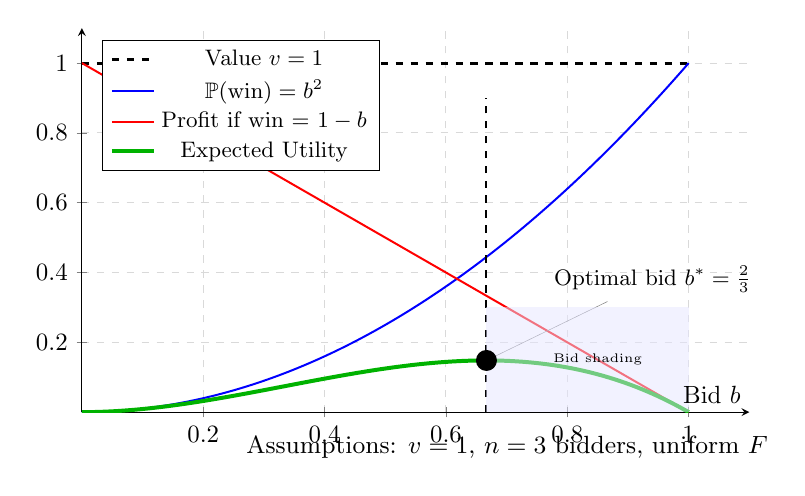
\begin{tikzpicture}[scale=0.9]
  \begin{axis}[
    xlabel={Bid $b$},
    ylabel={},
    xmin=0, xmax=1.1,
    ymin=0, ymax=1.1,
    axis lines=middle,
    legend pos=north west,
    legend style={fill=white, draw=black, font=\small},
    width=11cm,
    height=7cm,
    grid=major,
    grid style={dashed, gray!30}
  ]
  
  % Value v = 1
  \addplot[domain=0:1, samples=2, very thick, black, dashed] {1};
  \addlegendentry{Value $v = 1$}
  
  % Probability of winning: F^(n-1)(b) = b^2 for n=3, uniform
  \addplot[domain=0:1, samples=100, thick, blue] {x^2};
  \addlegendentry{$\mathbb{P}(\text{win}) = b^2$}
  
  % Profit if win: v - b = 1 - b
  \addplot[domain=0:1, samples=100, thick, red] {1-x};
  \addlegendentry{Profit if win = $1 - b$}
  
  % Expected utility: (v - b) * F^(n-1)(b) = (1-b)*b^2
  \addplot[domain=0:1, samples=100, ultra thick, green!70!black] {(1-x)*x^2};
  \addlegendentry{Expected Utility}
  
  % Optimal bid: maximize (1-b)*b^2
  % FOC: -b^2 + 2b(1-b) = 0 => -b^2 + 2b - 2b^2 = 0 => 2b - 3b^2 = 0 => b(2 - 3b) = 0 => b = 2/3
  \addplot[mark=*, mark size=4pt, only marks, black] coordinates {(0.6667,0.1481)};
  \node[pin={[pin distance=1cm]45:{\small Optimal bid $b^* = \frac{2}{3}$}}] at (axis cs:0.6667,0.1481) {};
  
  % Vertical line at optimal
  \draw[dashed, thick] (axis cs:0.6667,0) -- (axis cs:0.6667,0.9);
  
  % Shading region
  \fill[blue!10, opacity=0.5] (axis cs:0.6667,0) rectangle (axis cs:1,0.3);
  \node at (axis cs:0.85,0.15) {\tiny Bid shading};
  
  \end{axis}
  
  \node[align=center] at (6,-0.5) {\small Assumptions: $v = 1$, $n = 3$ bidders, uniform $F$};
\end{tikzpicture}
\end{center}
\end{frame}


\begin{frame}{First-Price: Equilibrium Derivation}
\textbf{Maximization Problem:}
If bidder $i$ with value $v_i$ bids as if value $w_i$:
$$\E[U_i] = (v_i - B(w_i)) \cdot F^{n-1}(w_i)$$


\textbf{First-Order Condition:}
$$\frac{\partial}{\partial w_i}: (v_i - B(w_i))(n-1)f(w_i)F^{n-2}(w_i) - B'(w_i)F^{n-1}(w_i) = 0$$

At symmetric equilibrium $w_i = v_i$:
$$B'(v_i) = (n-1)(v_i - B(v_i))\frac{f(v_i)}{F(v_i)}$$

\textbf{General Solution:} (with $B(\underline{v}) = \underline{v}$)
$$B(v_i) = \frac{\int_{\underline{v}}^{v_i} t \, dF^{n-1}(t)}{F^{n-1}(v_i)} = v_i - \frac{\int_{\underline{v}}^{v_i} F^{n-1}(t)dt}{F^{n-1}(v_i)}$$

Note: $B(v_i) < v_i$ (always shade bid)
\end{frame}

\begin{frame}{First-Price: Uniform Distribution Example}
\textbf{Setup:} $v \sim U[0,1]$, so $F(v) = v$, $f(v) = 1$

\textbf{Differential equation:}
$$B'(v_i) = \frac{(n-1)(v_i - B(v_i))}{v_i}$$

\textbf{Guess linear solution:} $B(v_i) = kv_i$

Substituting: $k = \frac{(n-1)(v_i - kv_i)}{v_i} = (n-1)(1-k)$

Solving: $k = \frac{n-1}{n}$

\textbf{Equilibrium bid function:}
$$B(v_i) = \frac{n-1}{n} v_i$$

\textbf{Interpretation:}
\begin{itemize}
  \item 2 bidders: bid 50\% of value
  \item 10 bidders: bid 90\% of value  
  \item As $n \to \infty$: $B(v) \to v$ (competition eliminates shading)
\end{itemize}
\end{frame}


\begin{frame}{Visualization: Bid Functions Across Auction Types}
\begin{center}
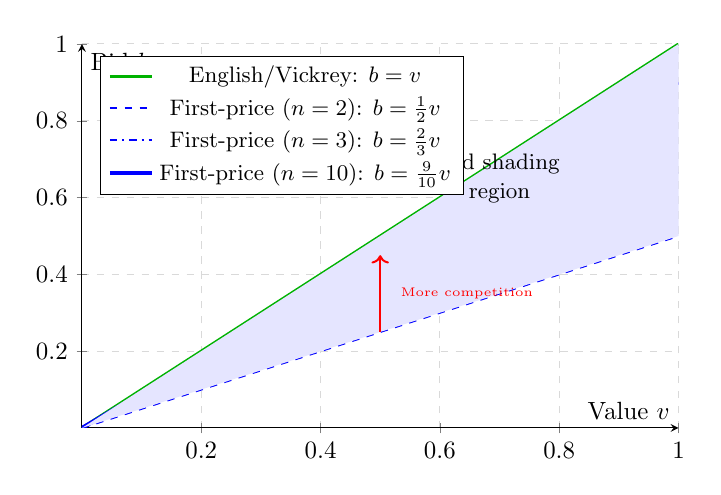
\begin{tikzpicture}[scale=0.9]
  \begin{axis}[
    xlabel={Value $v$},
    ylabel={Bid $b$},
    xmin=0, xmax=1,
    ymin=0, ymax=1,
    axis lines=middle,
    legend pos=north west,
    legend style={font=\small},
    width=10cm,
    height=7cm,
    samples=100,
    grid=major,
    grid style={dashed, gray!30}
  ]
  
  % 45-degree line (truthful bidding)
  \addplot[domain=0:1, very thick, green!70!black] {x};
  \addlegendentry{English/Vickrey: $b = v$}
  
  % First-price with n=2
  \addplot[domain=0:1, thick, blue, dashed] {0.5*x};
  \addlegendentry{First-price ($n=2$): $b = \frac{1}{2}v$}
  
  % First-price with n=3
  \addplot[domain=0:1, thick, blue, dashdotted] {0.667*x};
  \addlegendentry{First-price ($n=3$): $b = \frac{2}{3}v$}
  
  % First-price with n=10
  \addplot[domain=0:1, ultra thick, blue] {0.9*x};
  \addlegendentry{First-price ($n=10$): $b = \frac{9}{10}v$}
  
  % Shading area
  \fill[blue!10] (axis cs:0,0) -- (axis cs:1,0.5) -- (axis cs:1,1) -- (axis cs:0,0);
  \node[align=center] at (axis cs:0.7,0.65) {\small Bid shading\\\small region};
  
  % Arrow showing convergence
  \draw[->, thick, red] (axis cs:0.5,0.25) -- (axis cs:0.5,0.45);
  \node[right, red] at (axis cs:0.52,0.35) {\tiny More competition};
  
  \end{axis}
\end{tikzpicture}
\end{center}
\end{frame}


\begin{frame}{Derivation: First-Price Auction (Detailed)}
\begin{align*}
&v_i \sim F(v) - [\underline{v}, \bar{v}], \text{symmetric equilibrium} B(v) \text{ bids as if value } w: \\
&U(w; v_i) = (v_i - B(w)) \cdot F^{n-1}(w) \\
&\frac{\partial U}{\partial w} = -B'(w)F^{n-1}(w) + (v_i - B(w))(n-1)f(w)F^{n-2}(w) = 0 \\
&\text{Symmetric Equilibrium } (w = v_i): \\
&B'(v_i)F^{n-1}(v_i) = (v_i - B(v_i))(n-1)f(v_i)F^{n-2}(v_i) \\
&\rightarrow B'(v_i) = (n-1)(v_i - B(v_i))\frac{f(v_i)}{F(v_i)} \\
&\text{Solution (first-order linear ODE with } B(\underline{v}) = \underline{v}): \\
& B(v_i) = \frac{\int_{\underline{v}}^{v_i} t \, dF^{n-1}(t)}{F^{n-1}(v_i)} = v_i - \frac{\int_{\underline{v}}^{v_i} F^{n-1}(t)dt}{F^{n-1}(v_i)}
\end{align*}
\end{frame}


\begin{frame}{Derivation: First-Price Uniform Example}
\textbf{Setup:} $v_i \sim U[0,1]$, so $F(v) = v$, $f(v) = 1$

$$\text{ODE} B'(v_i) = (n-1)(v_i - B(v_i))\frac{1}{v_i}$$
\textbf{Guess Linear Solution:} $B(v_i) = \alpha v_i$ for some $\alpha \in [0,1]$

\begin{align*}
& \alpha = (n-1)(v_i - \alpha v_i)\frac{1}{v_i} = (n-1)(1 - \alpha) \\
& \rightarrow\alpha = \frac{n-1}{n} \\
& \rightarrow \boxed{B(v_i) = \frac{n-1}{n} v_i}
\end{align*}

\textbf{Verification:} Substitute back into ODE to confirm it satisfies the differential equation and boundary condition $B(0) = 0$. $\checkmark$
\end{frame}

\subsection{Sealed-Bid Second-Price }
\begin{frame}{What is a Second Price Auction?}
\begin{block}{Definition}
A \textbf{second price auction} is a \textbf{simultaneous} market mechanism where the highest bidder wins but pays the price bid by the second-highest bidder. 
\end{block}

\begin{exampleblock}{Sealed-Bid Second Price Format}
\begin{itemize}
\item Bidders submit sealed bids
\item Highest bid wins the item
\item Winner pays the second-highest bid
\end{itemize}
\end{exampleblock}

\begin{alertblock}{Note}
In a second price auction, bidding your true valuation is optimal. There is no incentive to bid strategically lower than your actual willingness to pay.
\end{alertblock}
\end{frame}

\begin{frame}{Second Price Dominant Strategy Theorem}
\begin{theorem}[Dominant Strategy]
In a second-price sealed-bid auction, bidding true valuation $b_i = v_i$ is a weakly dominant strategy for all bidders.
\end{theorem}
\textbf{Proof} Let $\tilde{b} = \max_{j \neq i} b_j$ (highest other bid)

\textbf{Case 1 Overbidding} $(b > v)$
\begin{itemize}
    \item If $\tilde{b}> v$, then you don't want to win
    \item If $\tilde{b}< v$, you can also win by bidding $b=v$, payoff is same $v-\tilde{b}>0$
\end{itemize}
Bidding $v$ dominates avoids losses, keeps all gains

\textbf{Case 2 Underbidding} $(b < v)$
\begin{itemize}
  \item If $v > \tilde{b} > b$ Lose, but could win profitably by bidding higher
  \item If $v > b > \tilde{b}$ Win with same profit as bidding $v$ 
\end{itemize}
Bidding $v$ dominates captures all profitable opportunities $\square$
\end{frame}

\begin{frame}{Information Flow in Different Formats}
\begin{center}
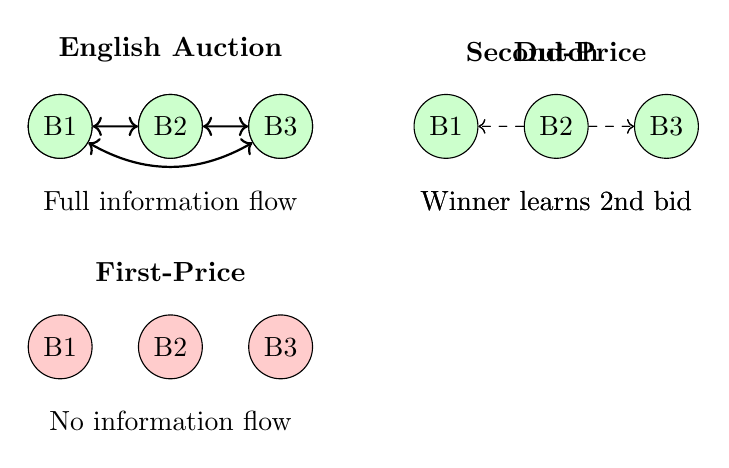
\begin{tikzpicture}[scale=0.7]
  % English Auction
  \node[draw, circle, fill=blue!20] (e1) at (0,4) {B1};
  \node[draw, circle, fill=blue!20] (e2) at (2,4) {B2};
  \node[draw, circle, fill=blue!20] (e3) at (4,4) {B3};
  \node[above] at (2,5) {\textbf{English Auction}};
  \draw[<->, thick] (e1) -- (e2);
  \draw[<->, thick] (e2) -- (e3);
  \draw[<->, thick] (e1) to[bend right] (e3);
  \node[below] at (2,3) {Full information flow};
  
  % Second-Price
  \node[draw, circle, fill=green!20] (s1) at (7,4) {B1};
  \node[draw, circle, fill=green!20] (s2) at (9,4) {B2};
  \node[draw, circle, fill=green!20] (s3) at (11,4) {B3};
  \node[above] at (9,5) {\textbf{Second-Price}};
  \draw[->, dashed] (s2) -- (s1);
  \draw[->, dashed] (s2) -- (s3);
  \node[below] at (9,3) {Winner learns 2nd bid};
  
  % First-Price
  \node[draw, circle, fill=red!20] (f1) at (0,0) {B1};
  \node[draw, circle, fill=red!20] (f2) at (2,0) {B2};
  \node[draw, circle, fill=red!20] (f3) at (4,0) {B3};
  \node[above] at (2,1) {\textbf{First-Price}};
  \node[below] at (2,-1) {No information flow};

  % Dutch auction
  \node[draw, circle, fill=green!20] (d1) at (0,4) {B1};
  \node[draw, circle, fill=green!20] (d2) at (2,4) {B2};
  \node[draw, circle, fill=green!20] (d3) at (4,4) {B3};
  \node[above] at (9,5) {\textbf{Dutch}};
  \draw[->, dashed] (s2) -- (s1);
  \draw[->, dashed] (s2) -- (s3);
  \node[below] at (9,3) {Winner learns 2nd bid};

\end{tikzpicture}
\end{center}

\textbf{Information Revelation Impact:}
\begin{itemize}
  \item More information $\rightarrow$ Less winner's curse
  \item Less winner's curse $\rightarrow$ More aggressive bidding
  \item More aggressive bidding $\rightarrow$ Higher revenue
\end{itemize}
\end{frame}

\subsection{All Pay}

\begin{frame}{What is an All-Pay Auction?}
\begin{block}{Definition}
An \textbf{all-pay auction} is a \textbf{simultaneous} market mechanism where the highest bidder wins the item, but \textbf{all bidders pay their bids} regardless of whether they win or lose.
\end{block}
\begin{exampleblock}{Sealed-Bid All-Pay Format}
\begin{itemize}
\item Bidders submit sealed bids
\item Highest bid wins the item
\item \textbf{All bidders pay their bid} (winner and losers)
\item Winner receives the item, losers receive nothing
\end{itemize}
\end{exampleblock}
\begin{alertblock}{Note}
All-pay auctions model situations like lobbying, R\&D races, and contests where effort is expended regardless of success. Bidders bid much more conservatively than in standard auctions since losing is costly.
\end{alertblock}
\end{frame}

\begin{frame}{All-Pay Auction: The Strategic Challenge}
\begin{center}
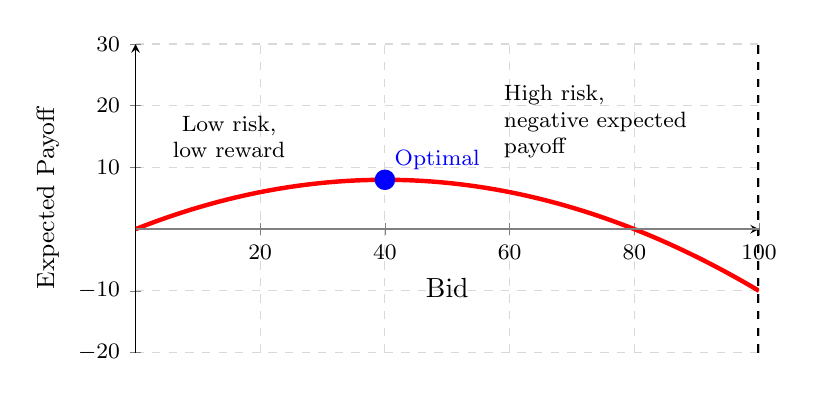
\begin{tikzpicture}[scale=1]
  \begin{axis}[
    xlabel={Bid},
    ylabel={Expected Payoff},
    xmin=0, xmax=100,
    ymin=-20, ymax=30,
    axis lines=middle,
    width=9.5cm,
    height=5.5cm,
    grid=major,
    grid style={dashed, gray!30},
    xtick={0,20,40,60,80,100},
    ytick={-20,-10,0,10,20,30},
    xlabel style={font=\small},
    xlabel near ticks, 
    ylabel near ticks, 
    ylabel style={font=\small},
    tick label style={font=\footnotesize}
  ]
  
  % True value line
  \addplot[domain=0:100, samples=2, very thick, black, dashed] coordinates {(100,-20) (100,30)};
  \node[font=\footnotesize] at (axis cs:100,32) {Your Value \$100K};
  
  % Expected payoff curve (much flatter and lower)
  \addplot[domain=0:100, samples=100, ultra thick, red] {-0.005*(x-40)^2 + 8};
  
  % Optimal bid marker
  \addplot[mark=*, mark size=3.5pt, only marks, blue] coordinates {(40,8)};
  \node[above right, blue, font=\footnotesize] at (axis cs:40,8) {Optimal};
  
  % Annotations
  \node[above, align=center, font=\footnotesize] at (axis cs:15,10) {Low risk,\\low reward};
  \node[above left, align=left, font=\footnotesize] at (axis cs:90,10) {High risk,\\negative expected\\payoff};
  
  % Zero line emphasis
  \addplot[domain=0:100, samples=2, thick, gray] coordinates {(0,0) (100,0)};
  
  \end{axis}
\end{tikzpicture}
\end{center}

\textbf{Key Insight:} Since you pay even if you lose, optimal bids are much lower than in standard auctions. Risk of loss constrains bidding behavior.
\end{frame}

\begin{frame}{All-Pay Auctions in Practice: Lobbying and Contests}
\textbf{Real-World Applications}
\begin{itemize}
  \item \textbf{Political lobbying:} Campaign contributions spent regardless of outcome
  \item \textbf{R\&D races:} Research costs incurred by all firms, only winner profits
  \item \textbf{Legal battles:} Legal fees paid by all parties, winner takes all
  \item \textbf{Sports tournaments:} Training costs for all athletes, prizes only for winners
\end{itemize}

\textbf{Example: Pharmaceutical R\&D}
\begin{center}
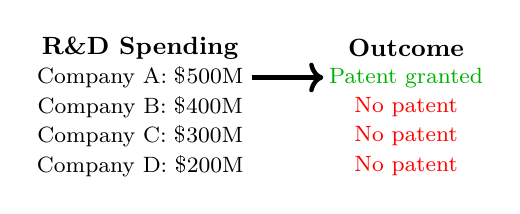
\begin{tikzpicture}[scale=0.75]
  % Companies
  \node[font=\small] at (2,3.0) {\textbf{R\&D Spending}};
  \node[font=\footnotesize] at (2,2.5) {Company A: \$500M};
  \node[font=\footnotesize] at (2,2.0) {Company B: \$400M};
  \node[font=\footnotesize] at (2,1.5) {Company C: \$300M};
  \node[font=\footnotesize] at (2,1.0) {Company D: \$200M};
  
  % Outcomes
  \node[font=\small] at (6.5,3.0) {\textbf{Outcome}};
  \node[font=\footnotesize, green!70!black] at (6.5,2.5) {Patent granted};
  \node[font=\footnotesize, red] at (6.5,2.0) {No patent};
  \node[font=\footnotesize, red] at (6.5,1.5) {No patent};
  \node[font=\footnotesize, red] at (6.5,1.0) {No patent};
  
  % Arrow
  \draw[ultra thick, ->] (3.9,2.5) -- (5.1,2.5);
\end{tikzpicture}
\end{center}

\textbf{Strategic Implication:} Firms must balance investment level against probability of success, knowing sunk costs are irrecoverable.
\end{frame}


\begin{frame}{All-Pay Auctions}
\textbf{Rules:}
\begin{itemize}
\item Highest bidder wins with certainty
\item All bidders pay their bids (non-refundable)
\item Applications: Patent races, political lobbying
\end{itemize}

\textbf{Symmetric Equilibrium:}
$$b(v_i) = \int_{\underline{v}}^{v_i} t dF^{N-1}(t) = v_i F^{N-1}(v_i) - \int_{\underline{v}}^{v_i} F^{N-1}(t)dt$$

\textbf{Uniform Distribution Example:} $v \sim U[0,1]$
$$b(v_i) = \frac{N-1}{N} v_i^N$$

Compare to first-price auction: $b_{FPA}(v_i) = \frac{N-1}{N} v_i$

Note: $b_{FPA}(v_i) > b_{All-Pay}(v_i)$ for all $v_i < 1$

\textbf{Revenue Equivalence:} $ER_{All-Pay} = E(v_{(2)})$
\end{frame}


\begin{frame}{War of Attrition}
\textbf{Second-Price All-Pay Auction:}
\begin{itemize}
\item Highest bidder wins
\item Winner pays second-highest bid
\item All losers pay their own bids
\item Application: Animal contests, standards wars
\end{itemize}

\textbf{Equilibrium Strategy:}
$$b(v_i) = -v_i \ln(1 - F^{N-1}(v_i)) + \int_{\underline{v}}^{v_i} \ln(1 - F^{N-1}(t))dt$$

\textbf{Two-Player Uniform Example:}
$$b(v_i) = -v_i - \ln(1-v_i)$$

Key property: $\lim_{v_i \to 1} b(v_i) = \infty$ (highest type bids infinity!)

\textbf{Revenue with Affiliation:}
$$ER_{War} \geq ER_{2nd-All-Pay} \geq ER_{1st-Price} = ER_{Dutch}$$
\end{frame}

\begin{frame}{Derivation: All-Pay First-Price Auction}
\textbf{Expected Utility:} If bidder with value $v_i$ bids as if value $w$:
\begin{align*}
&U(w; v_i) = v_i \cdot F^{n-1}(w) - B(w) && \text{Setup} \\
&\frac{\partial U}{\partial w} = v_i(n-1)f(w)F^{n-2}(w) - B'(w) = 0 && \text{FOC} \\
&B'(v_i) = v_i(n-1)f(v_i)F^{n-2}(v_i) && (w = v_i) \\
& B(v_i) = \int_{\underline{v}}^{v_i} t(n-1)f(t)F^{n-2}(t) \, dt = \int_{\underline{v}}^{v_i} t \, dF^{n-1}(t) && B(\underline{v}) = 0 \\
&B(v_i) = v_i F^{n-1}(v_i) - \int_{\underline{v}}^{v_i} F^{n-1}(t) \, dt && \text{By parts}
\end{align*}

\textbf{Uniform Distribution} ($F(v) = v$):
$$\boxed{B(v_i) = \frac{n-1}{n} v_i^n}$$
\end{frame}

\begin{frame}{Derivation: All-Pay First-Price Uniform Example}
\textbf{Setup:} $v_i \sim U[0,1]$, so $F(v) = v$
\begin{align*}
& B(v_i) = v_i F^{n-1}(v_i) - \int_0^{v_i} F^{n-1}(t) \, dt && \text{From above} \\
& B(v_i) = v_i \cdot v_i^{n-1} - \int_0^{v_i} t^{n-1} \, dt && F(t) = t \\
& B(v_i) = v_i^n - \left[\frac{t^n}{n}\right]_0^{v_i} && \\
& \boxed{B(v_i) = \frac{n-1}{n} v_i^n}  &&
\end{align*}

\textbf{Key Properties:}
\begin{itemize}
  \item $B(v_i) < v_i$ for all $v_i < 1$ (bid shading is severe)
  \item $B'(v_i) = (n-1)v_i^{n-1} > 0$ (increasing in value)
  \item $B(1) = \frac{n-1}{n}$ (highest type bids close to value)
  \item Expected payment: $\mathbb{E}[B(v)] = \frac{n-1}{n(n+1)}$
\end{itemize}
\end{frame}

\subsection{All Pay Second price/War of attrition}
\begin{frame}{What is an All-Pay Second Price Auction}
\begin{block}{Definition}
An \textbf{all-pay second price auction} (also called \textbf{war of attrition}) is a \textbf{simultaneous} market mechanism where the highest bidder wins and pays the \textbf{second-highest bid}, \\
but \textbf{all losing bidders also pay their own bids}.
\end{block}
\begin{exampleblock}{Sealed-Bid All-Pay Second Price Format}
\begin{itemize}
\item Bidders submit sealed bids
\item Highest bid wins the item
\item Winner pays the \textbf{second-highest bid}
\item \textbf{All losers pay their own bids}
\end{itemize}
\end{exampleblock}
\end{frame}

\begin{frame}{War of Attrition: Strategic Dynamics}
\textbf{The Unique Challenge}
\begin{itemize}
  \item Winner pays less than their bid (second-price benefit)
  \item But losers still pay their full bids (all-pay cost)
  \item Creates complex strategic trade-offs
\end{itemize}

\begin{center}
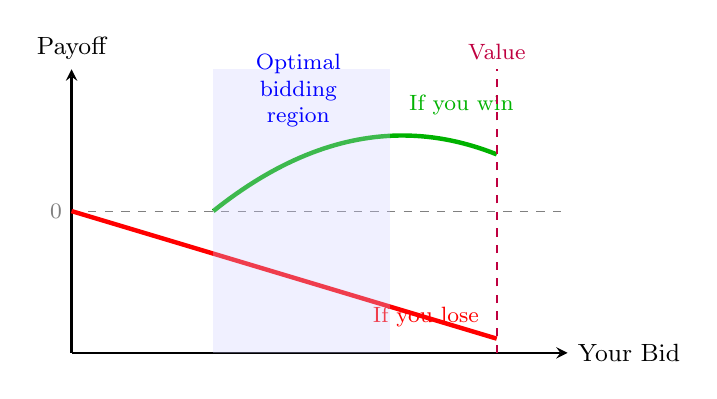
\begin{tikzpicture}[scale=0.9]
  % Set up axes
  \draw[thick, ->, >=stealth] (0,0) -- (7,0) node[right, font=\small] {Your Bid};
  \draw[thick, ->, >=stealth] (0,0) -- (0,4) node[above, font=\small] {Payoff};
  
  % Zero line
  \draw[dashed, gray] (0,2) -- (7,2);
  \node[left, gray, font=\footnotesize] at (0,2) {0};
  
  % Expected payoff curves
  % If you win (green)
  \draw[ultra thick, green!70!black] 
    plot[domain=2:6, samples=50] (\x, {2 + 0.8*(\x-2) - 0.15*(\x-2)^2});
  \node[green!70!black, font=\footnotesize] at (5.5,3.5) {If you win};
  
  % If you lose (red)
  \draw[ultra thick, red] 
    plot[domain=0:6, samples=50] (\x, {2 - 0.3*\x});
  \node[red, font=\footnotesize] at (5,0.5) {If you lose};
  
  % Optimal region
  \fill[blue!20, opacity=0.3] (2,0) rectangle (4.5,4);
  \node[blue, font=\footnotesize, align=center] at (3.2,3.7) {Optimal\\bidding\\region};
  
  % Value line
  \draw[dashed, purple, thick] (6,0) -- (6,4);
  \node[above, purple, font=\footnotesize] at (6,4) {Value};
\end{tikzpicture}
\end{center}

\textbf{Key Insight:} Optimal bid balances: (1) winning probability, (2) payment if winning (2nd price), (3) loss if losing (your bid)
\end{frame}

\begin{frame}{War of Attrition in Business: Market Competition}
\textbf{Real-World Applications}
\begin{itemize}
  \item \textbf{Price wars:} Firms sustain losses while competing; survivor gains market
  \item \textbf{Patent races:} All firms pay development costs; winner gets patent protection
  \item \textbf{Standard-setting battles:} All invest in promotion; winner sets industry standard
  \item \textbf{Market entry deterrence:} Incumbents and challengers burn resources
\end{itemize}

\textbf{Example: Streaming Service Price War}
\begin{center}
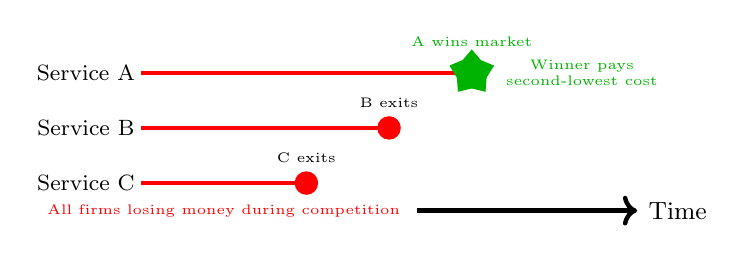
\begin{tikzpicture}[scale=0.70]
  % Timeline
  \draw[ultra thick, ->] (6,0) -- (10,0) node[right, font=\small] {Time};
  
  % Firms
  \node[font=\footnotesize] at (0,2.5) {Service A};
  \node[font=\footnotesize] at (0,1.5) {Service B};
  \node[font=\footnotesize] at (0,0.5) {Service C};
  
  % Costs during competition
  \draw[ultra thick, red] (1,2.5) -- (7,2.5);
  \draw[ultra thick, red] (1,1.5) -- (5.5,1.5);
  \draw[ultra thick, red] (1,0.5) -- (4,0.5);
  
  % Exit points
  \node[circle, fill=red, inner sep=3pt] at (4,0.5) {};
  \node[above, font=\tiny] at (4,0.7) {C exits};
  
  \node[circle, fill=red, inner sep=3pt] at (5.5,1.5) {};
  \node[above, font=\tiny] at (5.5,1.7) {B exits};
  
  % Winner
  \node[star, star points=5, fill=green!70!black, inner sep=4pt] at (7,2.5) {};
  \node[above, font=\tiny, green!70!black] at (7,2.8) {A wins market};
  
  % Cost annotations
  \node[red, font=\tiny] at (2.5,0) {All firms losing money during competition};
  \node[green!70!black, font=\tiny, align=center] at (9,2.5) {Winner pays\\second-lowest cost};
\end{tikzpicture}
\end{center}

\end{frame}


\begin{frame}{Derivation: War of Attrition (All-Pay Second-Price)}

$$U(w; v_i) = \mathbb{P}(\text{win}) \cdot (v_i - \mathbb{E}[\text{2nd bid} \mid \text{win}]) - \mathbb{P}(\text{lose}) \cdot B(w)$$

With symmetric strategies $B(\cdot)$:
\begin{align*}
U(w; v_i) &= F^{n-1}(w) \cdot v_i - \int_{\underline{v}}^w B(t) dF^{n-1}(t) - (1-F^{n-1}(w))B(w) \\
\frac{\partial U}{\partial w} & = (n-1)f(w)F^{n-2}(w)v_i - B(w)(n-1)f(w)F^{n-2}(w) \\
\quad\quad\quad\quad &+ (n-1)f(w)F^{n-2}(w)B(w) - B'(w)(1-F^{n-1}(w)) = 0
\end{align*}

\textbf{Simplify at} $w = v_i$:
$$B'(v_i)(1-F^{n-1}(v_i)) = (n-1)f(v_i)F^{n-2}(v_i)v_i$$

$$B'(v_i) = \frac{(n-1)f(v_i)F^{n-2}(v_i)}{1-F^{n-1}(v_i)} v_i = x v_i$$
\end{frame}

\begin{frame}{Derivation: War of Attrition ODE Solution}
\begin{align*}
& B'(v_i) = x v_i;
\frac{d}{dv}[-\ln(1-F^{n-1}(v))] =  x \\
& \rightarrow B'(v_i) = -v_i \frac{d}{dv_i}\ln(1-F^{n-1}(v_i)) \\
& B(v_i) = -v_i\ln(1-F^{n-1}(v_i)) + \int_{\underline{v}}^{v_i} \ln(1-F^{n-1}(t)) \, dt;
B(\underline{v}) = 0 \\
& = -v_i\ln(1-v_i^{n-1}) + \int_0^{v_i} \ln(1-t^{n-1}) \, dt;
\textbf{Uniform: } F(v) = v \text{ on } [0,1] \\
& = -v_i\ln(1-v_i) + \int_0^{v_i} \ln(1-t) \, dt;
\textbf{Two-Player Case: } n=2 \\
& = -v_i\ln(1-v_i) - v_i + v_i\ln(1-v_i) + \int_0^{v_i} \frac{t}{1-t} \, dt 
\end{align*}

$$\boxed{B(v_i) = v_i + (1-v_i)\ln(1-v_i)}$$
\end{frame}

\subsection{Tullock contests}


\begin{frame}{Tullock Contests}
\textbf{Contest Success Function:}
$$p_i(x_i, x_{-i}) = \begin{cases}
\frac{x_i^r}{\sum_{j=1}^N x_j^r} & \text{if } \sum_j x_j > 0 \\
\frac{1}{N} & \text{otherwise}
\end{cases}$$

\textbf{Parameter $r$ interpretation:}
\begin{itemize}
\item $r \to 0$: Random lottery (effort irrelevant)
\item $r = 1$: Lottery contest (linear in effort)
\item $r \to \infty$: All-pay auction (deterministic)
\end{itemize}

\textbf{Symmetric Equilibrium:}
$$x^* = \frac{r(N-1)V}{N^2}$$

\textbf{Rent Dissipation:} Total effort = $\frac{r(N-1)}{N} \times V$

Existence requires: $r \leq 2$ for $N \geq 2$
\end{frame}

\begin{frame}{Optimal Prize Allocation}
\textbf{Moldovanu-Sela (2001): How many prizes?}

\textbf{Setup:}
\begin{itemize}
\item $k$ contestants with ability $c_i \sim F[m,1]$ (low $c$ = high ability)
\item Cost of effort $x_i$: $c_i\gamma(x_i)$
\item Prizes: $V_1 \geq V_2$, with $V_1 + V_2 = 1$
\item Designer maximizes total expected effort
\end{itemize}

\textbf{Key Results:}
\begin{itemize}
\item \textbf{Linear/Concave costs:} Single prize optimal
\item \textbf{Convex costs:} Multiple prizes may be optimal
\end{itemize}

\textbf{Intuition:}
\begin{itemize}
\item First prize: Increases effort of high-ability types
\item Second prize: Motivates middle/low-ability types
\item With convex costs, second effect can dominate
\end{itemize}
\end{frame}


\begin{frame}{Derivation: Tullock Contest - Setup}
\textbf{Contest Success Function (CSF):}
$$p_i(x_i, x_{-i}) = \begin{cases}
\frac{x_i^r}{\sum_{j=1}^n x_j^r} & \text{if } \sum_j x_j > 0 \\
\frac{1}{n} & \text{otherwise}
\end{cases}$$

\textbf{Parameters:}
\begin{itemize}
  \item $x_i \geq 0$: Effort/expenditure by contestant $i$
  \item $r > 0$: Decisiveness parameter (technology of conflict)
  \item $V$: Prize value (same for all contestants)
  \item Cost of effort: $c(x_i) = x_i$ (linear cost)
\end{itemize}

\textbf{Expected Utility:}
$$U_i(x_i, x_{-i}) = p_i(x_i, x_{-i}) \cdot V - x_i = \frac{x_i^r}{\sum_{j=1}^n x_j^r} \cdot V - x_i$$

\textbf{Goal:} Find symmetric Nash equilibrium where all players choose $x^* = x_i = x_j$ for all $i,j$
\end{frame}

\begin{frame}{Derivation: Tullock Contest - FOC}
\textbf{Expected Utility of Player $i$:}
$$U_i = \frac{x_i^r}{x_i^r + \sum_{j \neq i} x_j^r} \cdot V - x_i$$

\textbf{In Symmetric Equilibrium:} All others choose $x_j = x^*$, so:
$$U_i = \frac{x_i^r}{x_i^r + (n-1)(x^*)^r} \cdot V - x_i$$

\textbf{First-Order Condition:}
$$\frac{\partial U_i}{\partial x_i} = V \cdot \frac{r x_i^{r-1}[x_i^r + (n-1)(x^*)^r] - x_i^r \cdot r x_i^{r-1}}{[x_i^r + (n-1)(x^*)^r]^2} - 1 = 0$$

\textbf{Simplify:}
$$\frac{\partial U_i}{\partial x_i} = V \cdot \frac{r x_i^{r-1} \cdot (n-1)(x^*)^r}{[x_i^r + (n-1)(x^*)^r]^2} - 1 = 0$$

\textbf{At Symmetric Equilibrium} ($x_i = x^*$):
$$V \cdot \frac{r (x^*)^{r-1} \cdot (n-1)(x^*)^r}{[x^* + (n-1)x^*]^2} = 1$$

$$V \cdot \frac{r(n-1)(x^*)^{2r-1}}{[n \cdot x^*]^2} = 1$$
\end{frame}

\begin{frame}{Derivation: Tullock Contest - Solution}
\textbf{From FOC:}
$$V \cdot \frac{r(n-1)(x^*)^{2r-1}}{n^2 (x^*)^{2r}} = 1$$

$$\frac{V \cdot r(n-1)}{n^2 \cdot x^*} = 1$$

\textbf{Solve for Equilibrium Effort:}
$$\boxed{x^* = \frac{r(n-1)V}{n^2}}$$

\textbf{Properties:}
\begin{itemize}
  \item \textbf{Comparative Statics:}
  \begin{itemize}
    \item $\frac{\partial x^*}{\partial V} > 0$: Higher prize $\Rightarrow$ more effort
    \item $\frac{\partial x^*}{\partial r} > 0$: More decisive contest $\Rightarrow$ more effort
    \item $\frac{\partial x^*}{\partial n} = \frac{rV(n-2)}{n^3}$: Non-monotonic in $n$
  \end{itemize}
  \item \textbf{Total Effort:} $n \cdot x^* = \frac{r(n-1)V}{n}$
  \item \textbf{Rent Dissipation:} $\frac{n \cdot x^*}{V} = \frac{r(n-1)}{n} \to r$ as $n \to \infty$
\end{itemize}

\textbf{Existence Condition:}
Second-order condition requires $r \leq 2$ for $n \geq 2$
\end{frame}

\begin{frame}{Derivation: Tullock Contest - Special Cases}
\textbf{Equilibrium Effort:} $x^* = \frac{r(n-1)V}{n^2}$


\textbf{Case 1: All-Pay Auction} ($r \to \infty$)
$$\lim_{r \to \infty} \frac{r(n-1)V}{n^2} = \infty$$
Contest becomes deterministic: highest effort wins with certainty


\textbf{Case 2: Pure Lottery} ($r \to 0$)
$$\lim_{r \to 0} \frac{r(n-1)V}{n^2} = 0$$
Effort doesn't matter: each player has probability $\frac{1}{n}$ regardless


\textbf{Case 3: Linear Contest} ($r = 1$)
$$x^* = \frac{(n-1)V}{n^2}$$

\textbf{Case 4: Two Players} ($n = 2$)
$$x^* = \frac{rV}{4}$$
Each player expends 25\% of prize value (when $r=1$)

\textbf{Total Rent Dissipation:} $2x^* = \frac{rV}{2}$ (50\% of prize when $r=1$)
\end{frame}


\subsection{Rank - Order Tournaments}

\begin{frame}{Rank-Order Tournaments}
\textbf{Lazear-Rosen (1981): Tournament vs. Piece Rates}

Output: $y_i = f(e_i) + \epsilon_{common} + \epsilon_i$

\textbf{Key Insights:}
\begin{itemize}
\item Risk-neutral agents: All schemes equivalent
\item Risk-averse agents:
  \begin{itemize}
  \item Large common shock $\Rightarrow$ Tournament better
  \item Large idiosyncratic shock $\Rightarrow$ Piece rates better
  \end{itemize}
\end{itemize}

\textbf{Green-Stokey (1983): Information Value}
\begin{itemize}
\item Tournaments filter common shocks via relative performance
\item Large groups: Ranking $\approx$ precise performance measure
\item Useful when common shock distribution unknown
\end{itemize}

\textbf{Practical advantages:}
\begin{itemize}
\item Easier to measure ranks than absolute output
\item Robust to non-stationary environments
\end{itemize}
\end{frame}

\begin{frame}{Elimination Tournaments}
\textbf{Rosen (1986): Sequential Contests}

\textbf{Key Finding:} Need disproportionately large top prize

\textbf{Option Value Logic:}
\begin{itemize}
\item Each stage: Winner gets option to continue
\item As stages progress, fewer opportunities remain
\item Final stage: No tomorrow $\Rightarrow$ option expires
\item Top prize must compensate for all expired options
\end{itemize}

\textbf{Behavioral Effects:}
\begin{itemize}
\item Pessimists: Underperform (appear weaker, value lower)
\item Optimists: Mixed (underestimate rivals vs. overvalue continuation)
\item Signaling incentives increase with prize concentration
\end{itemize}

\textbf{Application:} Executive compensation ladders
\end{frame}

\begin{frame}{Application: Litigation Systems}
\textbf{Baye-Kovenock-de Vries (2005): Fee-Shifting Rules}

\textbf{Legal Systems:}
\begin{itemize}
\item USA: Each pays own ($\alpha = \beta = 1$)
\item UK: Loser pays all ($\alpha = 1, \beta = 0$)
\item Continental: Mixed ($\alpha = 1, \beta \in (0,1)$)
\end{itemize}

\textbf{Equilibrium Expenditure:}
$$e(v) = \frac{\int_0^v t[\alpha - (\alpha-\beta)F(t)]dF(t)}{[\alpha - (\alpha-\beta)F(v)]^2}$$

\textbf{Results:}
\begin{itemize}
\item Per-trial costs: UK $>$ Continental $>$ USA
\item Settlement incentives: USA $>$ Continental $>$ UK
\item Total litigation: USA $>$ Continental $>$ UK
\end{itemize}

Key: USA system encourages more cases but lower per-case spending
\end{frame}

\begin{frame}{Application: Status Competition}
\textbf{Hopkins-Kornienko (2004, 2006): Growth and Inequality}

\textbf{Status concerns in consumption:}
$$U = \log S(c_i, F(c)) + \rho \log c_{i,t+1}$$
where $S(c_i, F) = S_0 + \delta F(c_i) + (1-\delta)F^-(c_i)$

\textbf{Equilibrium investment:}
$$k(z) = \frac{zS_0^\nu + \int_{\underline{z}}^z (S_0 + G(y))^\nu dy}{(S_0 + G(z))^\nu}$$

\textbf{Key Results:}
\begin{itemize}
\item "Harsh" competition ($S_0 = 0$): Redistribution $\downarrow$ growth
\item "Mild" competition ($S_0 > 0$): Redistribution may $\uparrow$ growth
\item Competitiveness effect can dominate scale effect
\end{itemize}
\end{frame}

\begin{frame}{Contest Success Functions: Visualization}
\begin{center}
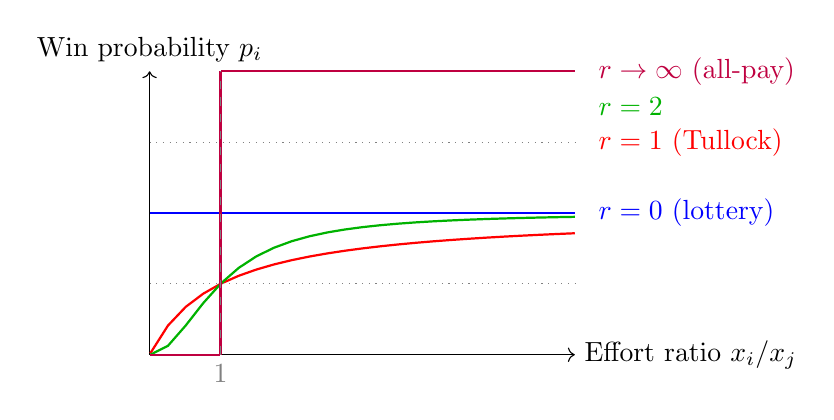
\begin{tikzpicture}[scale=0.9]
  \draw[->] (0,0) -- (6,0) node[right] {Effort ratio $x_i/x_j$};
  \draw[->] (0,0) -- (0,4) node[above] {Win probability $p_i$};
  
  % Different r values
  \draw[thick, blue] (0,2) -- (6,2);
  \node[blue, right] at (6.2,2) {$r=0$ (lottery)};
  
  \draw[thick, red, domain=0.01:6] plot (\x, {2*\x/(1+\x)});
  \node[red, right] at (6.2,3) {$r=1$ (Tullock)};
  
  \draw[thick, green!70!black, domain=0.01:6] plot (\x, {2*\x*\x/(1+\x*\x)});
  \node[green!70!black, right] at (6.2,3.5) {$r=2$};
  
  \draw[thick, purple] (0,0) -- (0.99,0) (1.01,4) -- (6,4);
  \draw[thick, purple] (1,0) -- (1,4);
  \node[purple, right] at (6.2,4) {$r \to \infty$ (all-pay)};
  
  \draw[dashed, gray] (1,0) -- (1,4);
  \draw[gray] (1,0) node[below] {1};
  
  % Add grid lines
  \draw[dotted, gray] (0,1) -- (6,1);
  \draw[dotted, gray] (0,3) -- (6,3);
\end{tikzpicture}
\end{center}
\end{frame}


\begin{frame}{Derivation: Rank-Order Tournament - Setup (Lazear-Rosen 1981)}
\textbf{Model:}
\begin{itemize}
  \item Two risk-averse workers: $i \in \{1, 2\}$
  \item Output: $q_i = e_i + \varepsilon_i + \theta$
  \begin{itemize}
    \item $e_i$: Effort (choice variable)
    \item $\varepsilon_i$: Idiosyncratic shock, $\varepsilon_i \sim N(0, \sigma_\varepsilon^2)$, independent
    \item $\theta$: Common shock, $\theta \sim N(0, \sigma_\theta^2)$
  \end{itemize}
  \item Prizes: $w_1 > w_2$ (winner and loser prizes)
  \item Utility: $u(w) - c(e)$ where $u'(w) > 0$, $u''(w) < 0$, $c'(e) > 0$, $c''(e) > 0$
  \item Cost of effort: $c(e) = \frac{1}{2}e^2$ (quadratic)
\end{itemize}

\textbf{Tournament Rule:}
$$\text{Worker } i \text{ wins if } q_i > q_j \Leftrightarrow e_i + \varepsilon_i > e_j + \varepsilon_j$$

\textbf{Goal:} Derive optimal prize spread $(w_1, w_2)$ and equilibrium effort
\end{frame}

\begin{frame}{Derivation: Rank-Order Tournament - Worker's Problem}
\textbf{Symmetric Equilibrium:} Both workers choose same effort $e^* = e_1 = e_2$

\textbf{Worker $i$'s Winning Probability:}
$$p_i = \mathbb{P}(q_i > q_j) = \mathbb{P}(e_i + \varepsilon_i + \theta > e_j + \varepsilon_j + \theta)$$
$$= \mathbb{P}(e_i + \varepsilon_i > e_j + \varepsilon_j) = \mathbb{P}(\varepsilon_i - \varepsilon_j > e_j - e_i)$$

In symmetric equilibrium ($e_i = e_j = e^*$):
$$p_i = \mathbb{P}(\varepsilon_i - \varepsilon_j > 0) = \frac{1}{2}$$

\textbf{Expected Utility:}
$$EU_i(e_i | e_j = e^*) = p_i(e_i, e^*) \cdot u(w_1) + (1-p_i(e_i, e^*)) \cdot u(w_2) - c(e_i)$$

\textbf{Note:} $\varepsilon_i - \varepsilon_j \sim N(0, 2\sigma_\varepsilon^2)$, so:
$$p_i(e_i, e_j) = \Phi\left(\frac{e_i - e_j}{\sqrt{2\sigma_\varepsilon^2}}\right) = \Phi\left(\frac{e_i - e_j}{\sigma_\varepsilon\sqrt{2}}\right)$$

where $\Phi(\cdot)$ is the standard normal CDF
vation: War of Attrition (All\end{frame}

\begin{frame}{Derivation: Rank-Order Tournament - FOC}
\textbf{Expected Utility:}
$$EU_i = \Phi\left(\frac{e_i - e^*}{\sigma_\varepsilon\sqrt{2}}\right) u(w_1) + \left[1-\Phi\left(\frac{e_i - e^*}{\sigma_\varepsilon\sqrt{2}}\right)\right] u(w_2) - \frac{1}{2}e_i^2$$

\textbf{First-Order Condition:}
$$\frac{\partial EU_i}{\partial e_i} = \phi\left(\frac{e_i - e^*}{\sigma_\varepsilon\sqrt{2}}\right) \cdot \frac{1}{\sigma_\varepsilon\sqrt{2}} \cdot [u(w_1) - u(w_2)] - e_i = 0$$

where $\phi(\cdot)$ is the standard normal PDF

\textbf{At Symmetric Equilibrium} ($e_i = e^* = e_j$):
$$\phi(0) \cdot \frac{1}{\sigma_\varepsilon\sqrt{2}} \cdot [u(w_1) - u(w_2)] = e^*$$

Since $\phi(0) = \frac{1}{\sqrt{2\pi}}$:

$$\frac{1}{\sqrt{2\pi}} \cdot \frac{1}{\sigma_\varepsilon\sqrt{2}} \cdot [u(w_1) - u(w_2)] = e^*$$

\textbf{Equilibrium Effort:}
$$\boxed{e^* = \frac{u(w_1) - u(w_2)}{\sigma_\varepsilon \cdot 2\sqrt{\pi}}}$$
\end{frame}

\begin{frame}{Derivation: Tournament vs Piece-Rate}
\textbf{Piece-Rate Compensation:} $w_i = \beta q_i + \alpha$
$$EU_i^{PR} = \mathbb{E}[u(\beta(e_i + \varepsilon_i + \theta) + \alpha)] - c(e_i)$$

\textbf{Risk-Neutral Case:}
\begin{itemize}
  \item Tournament: Effort depends on $\Delta u = u(w_1) - u(w_2)$ and $\sigma_\varepsilon$
  \item Piece-rate: Effort depends on $\beta$
  \item Both equivalent: Can set $\Delta u$ to induce same effort as optimal $\beta$
\end{itemize}

\textbf{Risk-Averse Case with Shocks:}

\textbf{Large Common Shock} ($\sigma_\theta^2$ large):
\begin{itemize}
  \item \textbf{Tournament better:} Common shock cancels in relative performance
  \item Worker bears less risk in tournament
  \item $q_i - q_j = e_i - e_j + \varepsilon_i - \varepsilon_j$ (no $\theta$!)
\end{itemize}

\textbf{Large Idiosyncratic Shock} ($\sigma_\varepsilon^2$ large):
\begin{itemize}
  \item \textbf{Piece-rate better:} Tournament adds noise to compensation
  \item High-performing worker may lose due to bad luck
  \item From FOC: $e^* \propto \frac{1}{\sigma_\varepsilon}$ (effort decreases with noise)
\end{itemize}
\end{frame}

\begin{frame}{Derivation: Optimal Prize Spread}
\textbf{Principal's Problem:} Choose $(w_1, w_2)$ to maximize profits subject to:
\begin{enumerate}
  \item Incentive Compatibility (IC): Worker chooses optimal effort
  \item Individual Rationality (IR): Worker accepts contract
\end{enumerate}

\textbf{Constraints:}
$$e^* = \frac{u(w_1) - u(w_2)}{\sigma_\varepsilon \cdot 2\sqrt{\pi}} \quad \text{(IC)}$$

$$\frac{1}{2}u(w_1) + \frac{1}{2}u(w_2) - c(e^*) \geq \bar{u} \quad \text{(IR)}$$

\textbf{Principal's Profit:}
$$\Pi = \mathbb{E}[q_1 + q_2] - (w_1 + w_2) = 2e^* - w_1 - w_2$$

\textbf{Lagrangian:}
$$\mathcal{L} = 2e^* - w_1 - w_2 + \lambda\left[\frac{1}{2}u(w_1) + \frac{1}{2}u(w_2) - c(e^*) - \bar{u}\right]$$

subject to IC constraint

\textbf{Key Result:} Optimal prize spread balances:
\begin{itemize}
  \item Higher spread $\Rightarrow$ more effort (good)
  \item Higher spread $\Rightarrow$ more risk for workers $\Rightarrow$ higher expected wage (bad)
\end{itemize}
\end{frame}

\begin{frame}{Derivation: Risk-Neutral Benchmark}
\textbf{If Workers Are Risk-Neutral:} $u(w) = w$

\textbf{Equilibrium Effort:}
$$e^* = \frac{w_1 - w_2}{\sigma_\varepsilon \cdot 2\sqrt{\pi}}$$

\textbf{Principal's Problem:}
$$\max_{w_1, w_2} \, 2e^* - w_1 - w_2$$
$$\text{s.t. } \frac{1}{2}w_1 + \frac{1}{2}w_2 - \frac{1}{2}(e^*)^2 \geq \bar{u}$$

\textbf{From IC:} $w_1 - w_2 = e^* \cdot \sigma_\varepsilon \cdot 2\sqrt{\pi}$

\textbf{FOC with respect to} $e^*$:
$$2 = \lambda e^* + \text{shadow price from IC}$$

\textbf{Solution:} Set prize spread to induce first-best effort $e^{FB}$ where:
$$\text{Marginal product} = \text{Marginal cost} \Rightarrow 1 = c'(e^{FB}) = e^{FB}$$

$$\boxed{e^* = 1, \quad w_1 - w_2 = \sigma_\varepsilon \cdot 2\sqrt{\pi}}$$

\textbf{Interpretation:} Prize spread compensates for noise in performance measurement
\end{frame}
\begin{frame}{Summary: Contests and Tournaments}
\textbf{Tullock Contest:}
\begin{itemize}
  \item Equilibrium effort: $x^* = \frac{r(n-1)V}{n^2}$
  \item Rent dissipation: $\frac{r(n-1)}{n}$ fraction of prize
  \item More decisive technology ($r$ higher) $\Rightarrow$ higher effort
  \item Inverted-U in number of contestants
\end{itemize}


\textbf{Rank-Order Tournament:}
\begin{itemize}
  \item Equilibrium effort: $e^* = \frac{u(w_1) - u(w_2)}{\sigma_\varepsilon \cdot 2\sqrt{\pi}}$
  \item Optimal prize spread balances incentives vs. risk
  \item Tournament dominates piece-rate when common shocks large
  \item Piece-rate dominates when idiosyncratic shocks large
\end{itemize}


\textbf{Key Insights:}
\begin{itemize}
  \item Contest technology ($r$) critically affects equilibrium behavior
  \item Relative performance evaluation filters common shocks
  \item Optimal mechanism depends on noise structure
\end{itemize}
\end{frame}

\subsection{Summary}
\begin{frame}{Summary: Bidding Functions - All Formats}
\textbf{Uniform Distribution} $v \sim U[0,1]$, $n$ bidders:

\begin{center}
\begin{tabular}{lcc}
\toprule
\textbf{Auction Format} & \textbf{Equilibrium Bid} $B(v)$ & \textbf{Revenue} \\
\midrule
English & $v$ & $\mathbb{E}[v_{(2)}] = \frac{n-1}{n+1}$ \\[0.2cm]
Second-Price & $v$ & $\mathbb{E}[v_{(2)}] = \frac{n-1}{n+1}$ \\[0.2cm]
First-Price & $\frac{n-1}{n}v$ & $\mathbb{E}[v_{(2)}] = \frac{n-1}{n+1}$ \\[0.2cm]
Dutch & $\frac{n-1}{n}v$ & $\mathbb{E}[v_{(2)}] = \frac{n-1}{n+1}$ \\[0.2cm]
All-Pay 1st & $\frac{n-1}{n}v^n$ & $\mathbb{E}[v_{(2)}] = \frac{n-1}{n+1}$ \\[0.2cm]
War of Attrition & $v + (1-v)\ln(1-v)$ & $\mathbb{E}[v_{(2)}] = \frac{n-1}{n+1}$ \\
& (for $n=2$) & \\
\bottomrule
\end{tabular}
\end{center}


\textbf{Key Observations:}
\begin{itemize}
  \item Revenue Equivalence holds under IPV, risk neutrality, symmetry
  \item Bid shading increases with: competition (larger $n$), all-pay structure
  \item Truth-telling optimal only in English and Second-Price formats
\end{itemize}
\end{frame}


\part{Assumptions}
\begin{frame}{Benchmark Model Setup}
\textbf{Three Key Assumptions:}
\begin{enumerate}
  \item \textbf{Independent Private Values (IPV):} 
  \begin{itemize}
    \item Valuations statistically independent
    \item Learning others' values doesn't change own value
  \end{itemize}
  \item \textbf{Risk Neutrality:} 
  \begin{itemize}
    \item Utility $U_i = v_i - b_i$ if win, 0 if lose
    \item No risk aversion or risk seeking
  \end{itemize}
  \item \textbf{Symmetry:} 
  \begin{itemize}
    \item All bidders from same distribution $F$
    \item No ex-ante differences between bidders
  \end{itemize}
\end{enumerate}

\textbf{Notation:}
\begin{itemize}
  \item $n$ bidders, valuations $v_i \sim F(v)$ on $[\underline{v}, \bar{v}]$
  \item Density $f(v) = F'(v)$, assume $f > 0$ on support
  \item Order statistics: $v_{(1)} \geq v_{(2)} \geq \cdots \geq v_{(n)}$
  \item Seller's valuation: $v_s = 0$ (for simplicity)
\end{itemize}
\end{frame}

\part{Results}

%===============================================
\section{Private Value Insights}
%===============================================

\begin{frame}{Strategic and Outcome Equivalence}
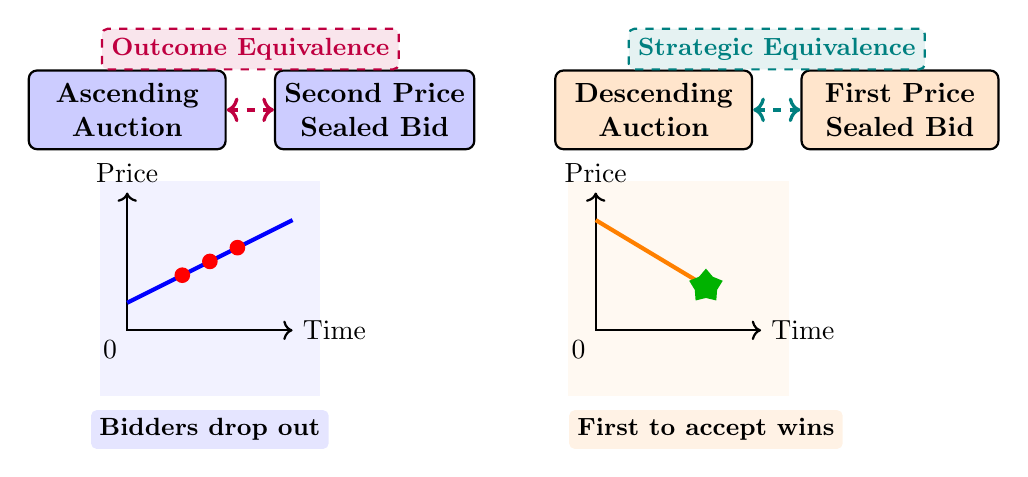
\begin{tikzpicture}[
    scale=0.7,
    % Define box styles
    auction/.style={
        rectangle,
        rounded corners=3pt,
        draw=black,
        thick,
        minimum width=2.5cm,
        minimum height=1cm,
        align=center,
        font=\bfseries
    },
    equiv/.style={
        rectangle,
        rounded corners=2pt,
        fill=white,
        draw=none,
        font=\small\bfseries
    }
]
    % =================================================================
    % --- TOP ROW Auction Types with Colored Boxes ---
    % =================================================================
    \node[auction, fill=blue!20] (eng_box) at (0, 0) {Ascending\\Auction};
    \node[auction, fill=blue!20, right=0.6cm of eng_box] (vickrey_box) {Second Price\\Sealed Bid};
    \node[auction, fill=orange!20, right=1cm of vickrey_box] (dutch_box) {Descending\\Auction};
    \node[auction, fill=orange!20, right=0.6cm of dutch_box] (firstprice_box) {First Price\\Sealed Bid};
    
    % Equivalence arrows with styled labels
    \draw[dashed, <->, line width=1.2pt, purple] (eng_box.east) -- (vickrey_box.west) 
        node[midway, above=0.5cm, equiv, fill=purple!10, draw=purple, thick] {Outcome Equivalence};
    
    \draw[dashed, <->, line width=1.2pt, teal] (dutch_box.east) -- (firstprice_box.west) 
        node[midway, above=0.5cm, equiv, fill=teal!10, draw=teal, thick] {Strategic Equivalence};
    
    % Ascending Auction Graph
    \begin{scope}[shift={(0, -4)}]
        % Background box
        \fill[blue!5] (-0.5, -1.2) rectangle (3.5, 2.7);
        
        \draw[thick, ->] (0, 2) -- (0, 0) node[below left] {0} -- (3, 0) node[right] {Time};
        \draw[thick, ->] (0, 0) -- (0, 2.5) node[above] {Price};
        \draw[thick, blue, line width=1.5pt] (0, 0.5) -- (1, 1) -- (2, 1.5) -- (3, 2);
        \foreach \x in {1, 1.5, 2} {
            \node[circle, fill=red, inner sep=2pt] at (\x, {0.5 + 0.5*\x}) {};
        }
        \node[font=\small\bfseries, fill=blue!10, rounded corners=2pt, inner sep=3pt] at (1.5, -1.8) {Bidders drop out};
    \end{scope}
    
    % Descending Auction Graph
    \begin{scope}[shift={(8.5, -4)}]
        % Background box
        \fill[orange!5] (-0.5, -1.2) rectangle (3.5, 2.7);
        
        \draw[thick, ->] (0, 2) -- (0, 0) node[below left] {0} -- (3, 0) node[right] {Time};
        \draw[thick, ->] (0, 0) -- (0, 2.5) node[above] {Price};
        \draw[thick, orange, line width=1.5pt] (0, 2) -- (2, 0.8);
        \node[star, star points=5, fill=green!70!black, inner sep=3pt] at (2, 0.8) {};
        \node[font=\small\bfseries, fill=orange!10, rounded corners=2pt, inner sep=3pt] at (2, -1.8) {First to accept wins};
    \end{scope}
\end{tikzpicture}
\end{frame}


\begin{frame}{Visualization: Bid Functions Across Auction Types}
\begin{center}
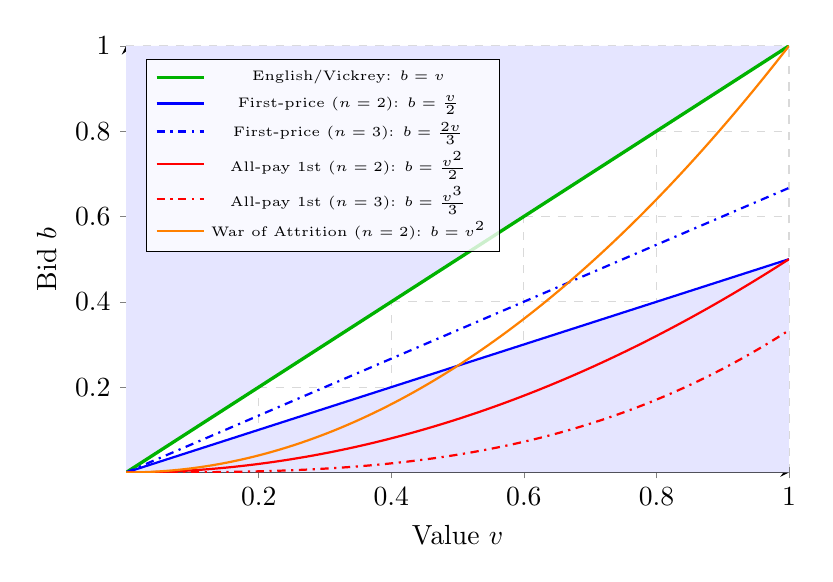
\begin{tikzpicture}[scale=1]
  \begin{axis}[
    xlabel={Value $v$},
    ylabel={Bid $b$},
    xmin=0, xmax=1,
    ymin=0, ymax=1,
    axis lines=middle,
    legend pos=north west,
    legend style={font=\tiny, fill=white, fill opacity=0.8, text opacity=1},
    width=10cm,
    height=7cm,
    xlabel near ticks, 
    ylabel near ticks, 
    samples=100,
    grid=major,
    grid style={dashed, gray!30}
  ]
  
  % Shading area (plot first so it's in background)
  \addplot[draw=none, fill=blue!10, domain=0:1, forget plot] {0.5*x} \closedcycle;
  \addplot[draw=none, fill=blue!10, domain=0:1, forget plot] {x} -- (axis cs:1,1) -- (axis cs:0,1) \closedcycle;
  
  % 45-degree line (truthful bidding)
  \addplot[domain=0:1, very thick, green!70!black] {x};
  \addlegendentry{English/Vickrey: $b = v$}
  
  % First-price with n=2
  \addplot[domain=0:1, thick, blue] {0.5*x};
  \addlegendentry{First-price ($n=2$): $b = \frac{v}{2}$}
  
  % First-price with n=3
  \addplot[domain=0:1, thick, blue, dashdotted] {0.667*x};
  \addlegendentry{First-price ($n=3$): $b = \frac{2v}{3}$}
  
  % All-pay first price with n=2
  \addplot[domain=0:1, thick, red] {x^2/2};
  \addlegendentry{All-pay 1st ($n=2$): $b = \frac{v^2}{2}$}
  
  % All-pay first price with n=3
  \addplot[domain=0:1, thick, red, dashdotted] {x^3/3};
  \addlegendentry{All-pay 1st ($n=3$): $b = \frac{v^3}{3}$}
  
  % War of Attrition (All-pay 2nd price) with n=2
  \addplot[domain=0:1, thick, orange] {x^2};
  \addlegendentry{War of Attrition ($n=2$): $b = v^2$}
  
  \end{axis}
\end{tikzpicture}
\end{center}

\vspace{-0.3cm}
{\small \textbf{Key insight 1:} All-pay auctions have more aggressive bid shading } \\
{\small \textbf{Key insight 2:} Mechanism determines effect of competition}
\end{frame}

\subsection{Revenue Equivalence}

\begin{frame}{The Big Surprise Revenue Equivalence}
\textbf{Amazing Result} Under standard conditions, all four formats generate the same expected revenue!

\begin{center}
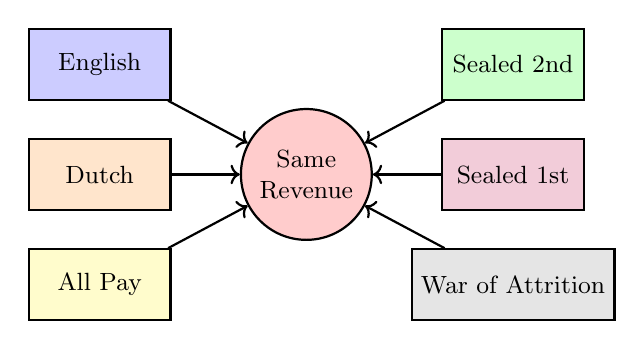
\begin{tikzpicture}[scale=0.70]
  % Four auction boxes
  \node[draw, thick, fill=blue!20, minimum width=1.8cm, minimum height=0.9cm, font=\small] (eng) at (-2,3) {English};
  \node[draw, thick, fill=green!20, minimum width=1.8cm, minimum height=0.9cm, font=\small] (vick) at (5.5,3) {Sealed 2nd};
  \node[draw, thick, fill=orange!20, minimum width=1.8cm, minimum height=0.9cm, font=\small] (dutch) at (-2,1) {Dutch};
  \node[draw, thick, fill=purple!20, minimum width=1.8cm, minimum height=0.9cm, font=\small] (first) at (5.5,1) {Sealed 1st};
  
  \node[draw, thick, fill=yellow!20, minimum width=1.8cm, minimum height=0.9cm, font=\small] (allp) at (-2,-1) {All Pay};
  \node[draw, thick, fill=gray!20, minimum width=1.8cm, minimum height=0.9cm, font=\small] (wot) at (5.5,-1) {War of Attrition};
  
  % Revenue
  \node[draw, circle, thick, fill=red!20, text width=1.2cm, align=center, font=\small] (rev) at (1.75,1) {Same \\ Revenue};
  
  % Arrows
  \draw[->, thick] (eng) -- (rev);
  \draw[->, thick] (vick) -- (rev);
  \draw[->, thick] (dutch) -- (rev);
  \draw[->, thick] (first) -- (rev);
  \draw[->, thick] (wot) -- (rev);
  \draw[->, thick] (allp) -- (rev);
\end{tikzpicture}
\end{center}

\textbf{Conditions Required}
\begin{itemize}
  \item Private values (each bidder knows their own value)
  \item Risk-neutral bidders
  \item No collusion
  \item Symmetric bidders (draw from same distribution)
\end{itemize}

\textbf{Implication} Choose format based on practical considerations, not revenue
\end{frame}


\begin{frame}{Expected Revenue Calculation}
\textbf{General Formula:}
$$ER = \int_{\underline{v}}^{\bar{v}} \text{[payment by winner]} \cdot \text{[probability density]} \, dv$$


\textbf{English \& Vickrey:} Winner pays $v_{(2)}$
$$ER_{SPA} = \E[v_{(2,n)}] = \int_{\underline{v}}^{\bar{v}} v \cdot g_{(2)}(v) \, dv$$
where $g_{(2)}$ is density of second-order statistic

\textbf{First-Price \& Dutch:} Winner pays $B(v_{(1)})$
$$ER_{FPA} = \int_{\underline{v}}^{\bar{v}} B(v) \cdot g_{(1)}(v) \, dv = \E[v_{(2,n)}]$$
(Can prove using integration by parts)

\textbf{Uniform Example:} Both equal $\frac{n-1}{n+1}$
\end{frame}

\begin{frame}{Revenue Equivalence Theorem (RET)}
\begin{theorem}[Vickrey 1961, Myerson 1981, Riley-Samuelson 1981]
Consider any two auction mechanisms satisfying:
\begin{enumerate}
  \item Bidders are risk-neutral with i.i.d. private values from $F$
  \item In equilibrium, object goes to bidder with highest value
  \item Bidder with lowest value $\underline{v}$ has zero expected surplus
\end{enumerate}
Then both mechanisms yield the same expected revenue to the seller.
\end{theorem}

\textbf{Remarkable Implication:}
$$ER_{English} = ER_{Vickrey} = ER_{Dutch} = ER_{First-Price} = \E[v_{(2)}]$$

\textbf{Intuition:}
\begin{itemize}
  \item Revenue determined by competition level, not payment rule
  \item Bidders adjust strategies to auction format
  \item In equilibrium, same economic forces prevail
\end{itemize}
\end{frame}

\begin{frame}{Visualization: Revenue Equivalence Intuition}
\begin{center}
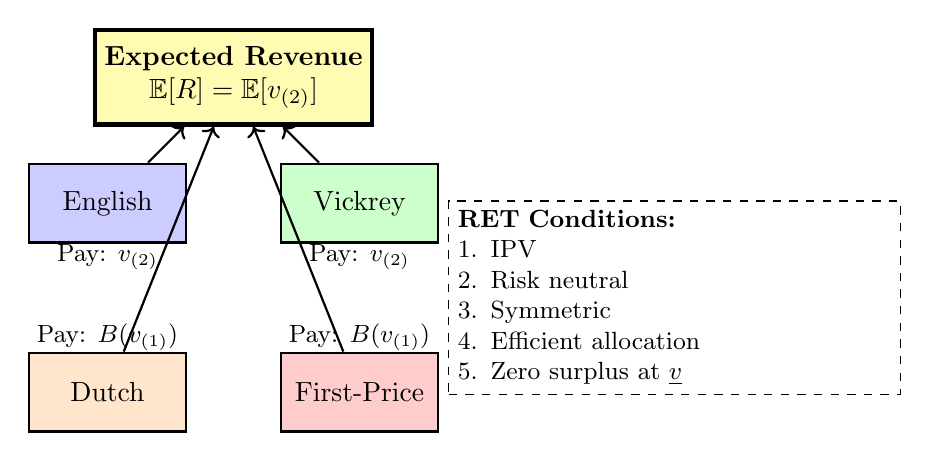
\begin{tikzpicture}[scale=0.8]
  % Four auction boxes
  \node[draw, thick, fill=blue!20, minimum width=2cm, minimum height=1cm] (eng) at (0,3) {English};
  \node[draw, thick, fill=green!20, minimum width=2cm, minimum height=1cm] (vick) at (4,3) {Vickrey};
  \node[draw, thick, fill=orange!20, minimum width=2cm, minimum height=1cm] (dutch) at (0,0) {Dutch};
  \node[draw, thick, fill=red!20, minimum width=2cm, minimum height=1cm] (fp) at (4,0) {First-Price};
  
  % Payment rules - moved further from boxes to avoid overlap
  \node[below, font=\small] at (0,2.5) {Pay: $v_{(2)}$};
  \node[below, font=\small] at (4,2.5) {Pay: $v_{(2)}$};
  \node[above, font=\small] at (0,0.5) {Pay: $B(v_{(1)})$};
  \node[above, font=\small] at (4,0.5) {Pay: $B(v_{(1)})$};
  
  % Central revenue box - slightly smaller to avoid overlap
  \node[draw, ultra thick, fill=yellow!30, minimum width=2.8cm, minimum height=1.2cm, align=center] (rev) at (2,5) {
    \textbf{Expected Revenue}\\
    $\E[R] = \E[v_{(2)}]$
  };
  
  % Arrows
  \draw[->, thick] (eng) -- (rev);
  \draw[->, thick] (vick) -- (rev);
  \draw[->, thick] (dutch) -- (rev);
  \draw[->, thick] (fp) -- (rev);
  
  % Conditions box
  \node[draw, dashed, text width=5.5cm, align=left, font=\small] at (9,1.5) {
    \textbf{RET Conditions:}\\
    1. IPV\\
    2. Risk neutral\\
    3. Symmetric\\
    4. Efficient allocation\\
    5. Zero surplus at $\underline{v}$
  };
\end{tikzpicture}
\end{center}
\end{frame}

\subsection{Auction Trilemma}

\begin{frame}{The Auction Trilemma You Can't Have It All}
\textbf{The Three Desirable Properties}

\begin{center}
\begin{figure}[h]
\centering
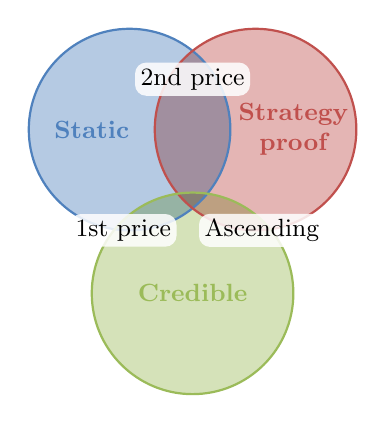
\begin{tikzpicture}[scale=1.6, every node/.style={font=\small}]
    % Define consistent colors
    \definecolor{staticcolor}{RGB}{79,129,189}      % blue
    \definecolor{stratproofcolor}{RGB}{192,80,77}   % red
    \definecolor{crediblecolor}{RGB}{155,187,89}    % green

    % Transparency layer
    \begin{scope}[blend group = multiply]
        \fill[staticcolor!60, opacity=0.7] (-0.5,0.8) circle (0.8cm);
        \fill[stratproofcolor!60, opacity=0.7] (0.5,0.8) circle (0.8cm);
        \fill[crediblecolor!60, opacity=0.7] (0,-0.5) circle (0.8cm);
    \end{scope}

    % Circle outlines
    
    \draw[thick, staticcolor] (-0.5,0.8) circle (0.8cm);
    \draw[thick, stratproofcolor] (0.5,0.8) circle (0.8cm);
    \draw[thick, crediblecolor] (0,-0.5) circle (0.8cm);

    % Labels for sets
    \node[font=\small\bfseries, staticcolor] at (-0.8,0.8) {Static};
    \node[font=\small\bfseries, stratproofcolor, align=center] at (0.8,0.8){Strategy\\proof};
    \node[font=\small\bfseries, crediblecolor] at (0,-0.5) {Credible};

    % Labels for intersections
    \node[align=center, fill=white, rounded corners, opacity=0.85, text opacity=1, inner sep=2pt]
        at (0,1.2) {2nd price};
    \node[align=center, fill=white, rounded corners, opacity=0.85, text opacity=1, inner sep=2pt]
        at (-0.55, 0) {1st price};
    \node[align=center, fill=white, rounded corners, opacity=0.85, text opacity=1, inner sep=2pt]
        at (0.55,0) {Ascending};
\end{tikzpicture}
\caption{An auction trilemma \textbf{Static} no time, all at once. \textbf{Strategy proof} no reason to bid anything other than your true value. \textbf{Credible} Auctioneer has no strategy to secretly get more revenue. Can't have all three}
\end{figure}

\end{center}

\end{frame}

\subsection{Reserve Prices}
\begin{frame}{Reserve Prices Almost Always Use Them}
\textbf{Reserve Price = Minimum acceptable bid}

\begin{center}
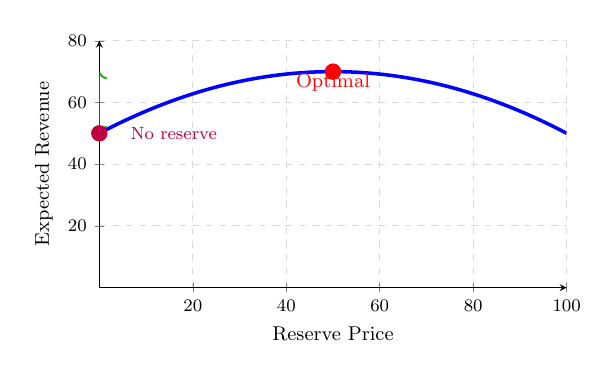
\begin{tikzpicture}[scale=0.80]
  \begin{axis}[
    xlabel={Reserve Price},
    ylabel={Expected Revenue},
    xmin=0, xmax=100,
    ymin=0, ymax=80,
    axis lines=middle,
    width=9cm,
    height=5.5cm,
    grid=major,
    grid style={dashed, gray!30},
    xtick={0,20,40,60,80,100},
    ytick={0,20,40,60,80},
    xlabel near ticks, 
    ylabel near ticks, 
    xlabel style={font=\small},
    ylabel style={font=\small},
    tick label style={font=\footnotesize}
  ]
  
  % Revenue curve
  \addplot[domain=0:100, samples=100, ultra thick, blue] {-0.008*(x-50)^2 + 70};
  
  % Optimal point
  \addplot[mark=*, mark size=3.5pt, only marks, red] coordinates {(50,70)};
  \node[below, red, font=\small] at (axis cs:50,72) {Optimal};
  
  % No reserve
  \addplot[mark=*, mark size=3.5pt, only marks, purple] coordinates {(0,50)};
  \node[right, purple, font=\footnotesize] at (axis cs:5,50) {No reserve};
  
  % Arrow showing gain
  \draw[<->, thick, green!70!black] (axis cs:0,50) -- (axis cs:0,70);
  \node[left, green!70!black, font=\footnotesize] at (axis cs:0,60) {+40\%};
  
  \end{axis}
\end{tikzpicture}
\end{center}


\textbf{Why They Work}
\begin{itemize}
  \item Forces bidders to compete more aggressively
  \item Protects against low-ball bids
  \item New Zealand spectrum disaster no reserve = \$1 winning bid!
\end{itemize}
\end{frame}


\begin{frame}{Entry Decisions and Participation}
\textbf{Endogenous Entry:}
\begin{itemize}
  \item Entry cost $c > 0$ to participate
  \item Symmetric equilibrium: enter with probability $p^*$
  \item Expected number of bidders: $n^* = Np^*$
\end{itemize}

\textbf{Optimal Auction with Entry:}
\begin{itemize}
  \item Reserve price affects entry incentives
  \item Too high $r$: Discourages entry
  \item Too low $r$: Excessive entry (wasteful)
  \item Optimal $r$ balances revenue vs. entry
\end{itemize}

\textbf{Entry Fees:}
\begin{itemize}
  \item Can screen out low-value bidders
  \item Revenue from fees + auction proceeds
  \item Optimal fee extracts entry rent
\end{itemize}
\end{frame}

\begin{frame}{Collusion and Bid Rigging}
\textbf{Forms of Collusion:}
\begin{itemize}
  \item Bid suppression: Some bidders don't bid
  \item Bid rotation: Take turns winning
  \item Cover bidding: Submit intentionally losing bids
\end{itemize}

\textbf{Factors Facilitating Collusion:}
\begin{itemize}
  \item Repeated interaction
  \item Small number of bidders
  \item Observable bids (English auction)
  \item Stable market conditions
\end{itemize}

\textbf{Anti-Collusion Mechanisms:}
\begin{itemize}
  \item Sealed-bid formats (harder to coordinate)
  \item Reserve prices (limit collusive gains)
  \item Random participation rules
  \item Legal penalties and monitoring
\end{itemize}
\end{frame}

\begin{frame}{Information Disclosure Policies}
\textbf{What to Reveal?}
\begin{itemize}
  \item Number of bidders
  \item Identities of participants
  \item Past winning bids
  \item Reserve price
\end{itemize}

\textbf{Trade-offs:}

\begin{tabular}{ll}
\toprule
\textbf{More Information} & \textbf{Less Information} \\
\midrule
$\uparrow$ Reduces uncertainty & $\uparrow$ Prevents collusion \\
$\uparrow$ Encourages participation & $\uparrow$ Strategic ambiguity \\
$\downarrow$ May facilitate collusion & $\downarrow$ May discourage entry \\
\bottomrule
\end{tabular}


\textbf{Optimal Policy:}
\begin{itemize}
  \item Depends on market characteristics
  \item Common values: More info generally better
  \item Private values with collusion risk: Less info better
\end{itemize}
\end{frame}


\begin{frame}{Summary: Core Results}
\textbf{1. Equilibrium Strategies:}
\begin{itemize}
  \item English/Vickrey: Bid true value (dominant strategy)
  \item First-Price/Dutch: Shade bid below value
  \item Shading depends on competition and distribution
\end{itemize}

\textbf{2. Revenue Equivalence (IPV, risk-neutral, symmetric):}
\begin{itemize}
  \item All standard formats yield same expected revenue
  \item Revenue = $\E[v_{(2)}]$ (expected second-highest value)
  \item Breaks with risk aversion, asymmetry, or correlation
\end{itemize}

\textbf{3. Optimal Design:}
\begin{itemize}
  \item Reserve price improves revenue
  \item Virtual valuation determines optimal allocation
  \item Standard auction + reserve achieves optimum
\end{itemize}
\end{frame}

\begin{frame}{Summary: Key Mathematical Results}
\begin{center}
\begin{tabular}{lcc}
\toprule
\textbf{Auction Type} & \textbf{Bid Strategy} & \textbf{Expected Revenue} \\
\midrule
English & $b = v$ & $\E[v_{(2)}]$ \\
Vickrey & $b = v$ & $\E[v_{(2)}]$ \\
First-Price & $b = \E[v_{(2)} | v_{(1)} = v]$ & $\E[v_{(2)}]$ \\
Dutch & $b = \E[v_{(2)} | v_{(1)} = v]$ & $\E[v_{(2)}]$ \\
\bottomrule
\end{tabular}
\end{center}


\textbf{Key Formulas:}
\begin{itemize}
  \item Optimal reserve: $r^* = v_s + \frac{1-F(r^*)}{f(r^*)}$
  \item Virtual valuation: $\psi(v) = v - \frac{1-F(v)}{f(v)}$
  \item First-price bid (uniform): $B(v) = \frac{n-1}{n}v$
  \item Risk averse bid: $B(v) = \frac{n-1}{n-(1-\gamma)}v$
\end{itemize}
\end{frame}

\begin{frame}{Key Insights for Practice}
\textbf{Choosing an Auction Format:}

\begin{tabular}{ll}
\toprule
\textbf{Use English/Ascending when:} & \textbf{Use Sealed-Bid when:} \\
\midrule
Common value elements & Preventing collusion important \\
Want price discovery & Speed matters \\
Affiliation present & Bidders geographically dispersed \\
Transparency important & Privacy concerns \\
\bottomrule
\end{tabular}


\textbf{Design Recommendations:}
\begin{itemize}
  \item Always set optimal reserve price
  \item Reveal information to reduce winner's curse
  \item First-price better with risk-averse bidders
  \item Consider entry fees and participation costs
  \item Multi-unit: Be aware of demand reduction
\end{itemize}

\textbf{Remember:} Real auctions rarely satisfy all RET assumptions!
\end{frame}

\section{Common value Insights}

%===============================================
\subsection{Common Values and Winner's Curse}
%===============================================

\begin{frame}{Pure Common Value Model}
\textbf{Setup:}
\begin{itemize}
  \item True value $V$ unknown to all at auction time
  \item Each bidder $i$ observes private signal $S_i$
  \item Signals correlated with true value
  \item Classic example: Oil drilling rights
\end{itemize}


\textbf{The Winner's Curse:}
\begin{itemize}
  \item Winning means you had the highest signal/estimate
  \item If signals unbiased: $\E[S_i] = V$
  \item But: $\E[V | S_i = s, \text{Win}] < s$ typically
  \item Naive bidding (based on $\E[V|S_i]$) leads to losses!
\end{itemize}


\textbf{Rational Response:}
\begin{itemize}
  \item Account for adverse selection of winning
  \item Bid conditional on being ``just winning''
  \item Shade bid more with more competitors
\end{itemize}
\end{frame}

\begin{frame}{Visualizing the Winner's Curse}
\begin{center}
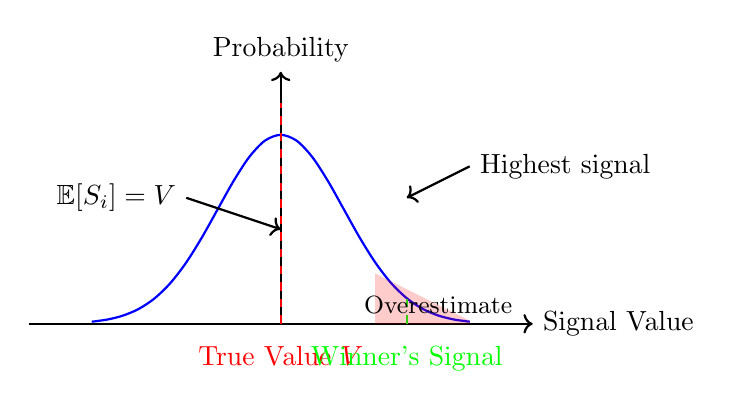
\begin{tikzpicture}[scale=0.8]
  % Draw normal distribution
  \draw[thick,->] (-4,0) -- (4,0) node[right] {Signal Value};
  \draw[thick,->] (0,0) -- (0,4) node[above] {Probability};
  
  % Draw bell curve
  \draw[thick,blue,domain=-3:3,smooth,variable=\x] plot ({\x},{3*exp(-\x*\x/2)});
  
  % Mark true value
  \draw[thick,red,dashed] (0,0) -- (0,3.5);
  \node[below,red] at (0,-0.2) {True Value $V$};
  
  % Mark winner's signal
  \draw[thick,green,dashed] (2,0) -- (2,0.5);
  \node[below,green] at (2,-0.2) {Winner's Signal};
  
  % Annotations
  \draw[<-,thick] (2,2) -- (3,2.5) node[right] {Highest signal};
  \draw[<-,thick] (0,1.5) -- (-1.5,2) node[left] {$\E[S_i] = V$};
  
  % Shaded area
  \fill[red,opacity=0.2] (1.5,0) -- (1.5,0.8) -- (3,0.05) -- (3,0) -- cycle;
  \node at (2.5,0.3) {\small Overestimate};
\end{tikzpicture}
\end{center}

\textbf{Key Insight:} The winner is the bidder with the most optimistic signal
\begin{itemize}
  \item Even with unbiased signals, winning is ``bad news''
  \item Must adjust bid downward to account for this selection effect
\end{itemize}
\end{frame}

\begin{frame}{Simple Common Value Example}
\textbf{Uniform Signal Model:}
\begin{itemize}
  \item Common value $V$
  \item Signals $t_i \sim U[V-\delta, V+\delta]$ independently
  \item $\E[V|t_i] = t_i$ (unbiased)
  \item $\E[V|\text{all signals}] = \frac{t_{(1)} + t_{(n)}}{2}$
\end{itemize}


\textbf{Equilibrium Strategies:}

\begin{tabular}{lll}
\toprule
Auction & Bid Function & Winner Pays \\
\midrule
Second-Price & $b(t_i) = t_i - \delta\frac{n-2}{n}$ & Second-highest bid \\
English & Update as others drop & $\frac{t_{(2)} + t_{(n)}}{2}$ \\
First-Price & $b(t_i) = t_i - \delta$ & Own bid \\
\bottomrule
\end{tabular}

\textbf{Note:} All bid below signal to avoid winner's curse!
\end{frame}

\begin{frame}{Winner's Curse: Theory and Evidence}
\textbf{Rational Response in Common Value Auctions:}

Bidder $i$ with signal $s_i$ should bid:
$$b(s_i) = \E[V | S_i = s_i, \max_{j \neq i} S_j = s_i] < \E[V | S_i = s_i]$$


\textbf{Experimental Evidence (Kagel \& Levin):}
\begin{itemize}
  \item Persistent overbidding even with experience
  \item Bankruptcy rates: 40-60\% in lab experiments
  \item Worse with more bidders (stronger adverse selection)
\end{itemize}


\textbf{Real-World Examples:}
\begin{itemize}
  \item \textbf{Oil lease auctions:} Average returns near zero for winners
  \item \textbf{Corporate takeovers:} Acquiring firm stock typically falls
  \item \textbf{Construction contracts:} Lowest bidder often loses money
\end{itemize}

\begin{tcolorbox}[colback=red!5!white,colframe=red!75!black,title=Mitigation Strategies]
Joint bidding, Information acquisition, Conservative bidding rules
\end{tcolorbox}
\end{frame}

%===============================================
\subsection{Information Revelation in Auctions}
%===============================================

\begin{frame}{Information Flow in Different Formats}
\begin{center}
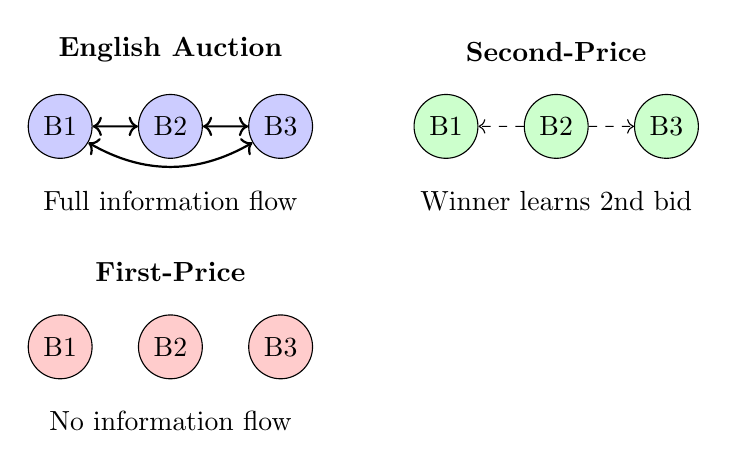
\begin{tikzpicture}[scale=0.7]
  % English Auction
  \node[draw, circle, fill=blue!20] (e1) at (0,4) {B1};
  \node[draw, circle, fill=blue!20] (e2) at (2,4) {B2};
  \node[draw, circle, fill=blue!20] (e3) at (4,4) {B3};
  \node[above] at (2,5) {\textbf{English Auction}};
  \draw[<->, thick] (e1) -- (e2);
  \draw[<->, thick] (e2) -- (e3);
  \draw[<->, thick] (e1) to[bend right] (e3);
  \node[below] at (2,3) {Full information flow};
  
  % Second-Price
  \node[draw, circle, fill=green!20] (s1) at (7,4) {B1};
  \node[draw, circle, fill=green!20] (s2) at (9,4) {B2};
  \node[draw, circle, fill=green!20] (s3) at (11,4) {B3};
  \node[above] at (9,5) {\textbf{Second-Price}};
  \draw[->, dashed] (s2) -- (s1);
  \draw[->, dashed] (s2) -- (s3);
  \node[below] at (9,3) {Winner learns 2nd bid};
  
  % First-Price
  \node[draw, circle, fill=red!20] (f1) at (0,0) {B1};
  \node[draw, circle, fill=red!20] (f2) at (2,0) {B2};
  \node[draw, circle, fill=red!20] (f3) at (4,0) {B3};
  \node[above] at (2,1) {\textbf{First-Price}};
  \node[below] at (2,-1) {No information flow};
\end{tikzpicture}
\end{center}

\textbf{Information Revelation Impact:}
\begin{itemize}
  \item More information $\rightarrow$ Less winner's curse
  \item Less winner's curse $\rightarrow$ More aggressive bidding
  \item More aggressive bidding $\rightarrow$ Higher revenue
\end{itemize}
\end{frame}

\begin{frame}{English Auction Information Dynamics}
\textbf{Progressive Information Revelation:}

\begin{center}
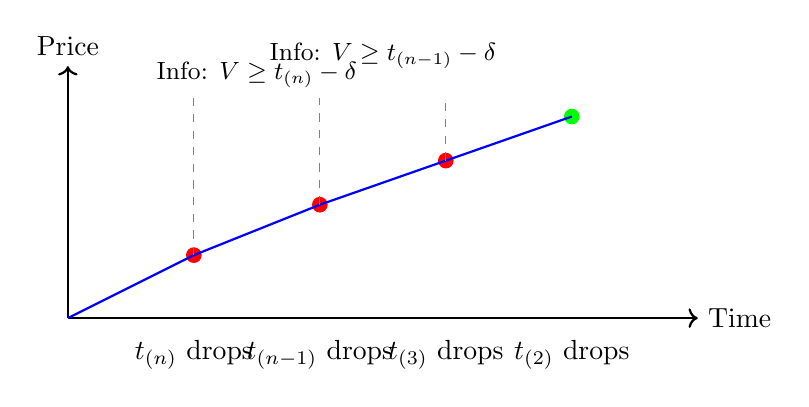
\begin{tikzpicture}[scale=0.8]
  % Timeline
  \draw[thick,->] (0,0) -- (10,0) node[right] {Time};
  
  % Price axis
  \draw[thick,->] (0,0) -- (0,4) node[above] {Price};
  
  % Dropout points
  \node[circle,fill=red,inner sep=2pt] (d1) at (2,1) {};
  \node[circle,fill=red,inner sep=2pt] (d2) at (4,1.8) {};
  \node[circle,fill=red,inner sep=2pt] (d3) at (6,2.5) {};
  \node[circle,fill=green,inner sep=2pt] (win) at (8,3.2) {};
  
  % Labels
  \node[below] at (2,-0.2) {$t_{(n)}$ drops};
  \node[below] at (4,-0.2) {$t_{(n-1)}$ drops};
  \node[below] at (6,-0.2) {$t_{(3)}$ drops};
  \node[below] at (8,-0.2) {$t_{(2)}$ drops};
  
  % Price path
  \draw[thick,blue] (0,0) -- (2,1) -- (4,1.8) -- (6,2.5) -- (8,3.2);
  
  % Information sets
  \draw[dashed,gray] (2,1) -- (2,3.5);
  \draw[dashed,gray] (4,1.8) -- (4,3.5);
  \draw[dashed,gray] (6,2.5) -- (6,3.5);
  
  \node[above,font=\small] at (3,3.5) {Info: $V \geq t_{(n)}-\delta$};
  \node[above,font=\small] at (5,3.8) {Info: $V \geq t_{(n-1)}-\delta$};
\end{tikzpicture}
\end{center}

\textbf{Belief Updates:}
\begin{itemize}
  \item Each dropout reveals that bidder's signal
  \item Remaining bidders update: $\E[V|\text{history}]$ increases
  \item Final two bidders have nearly complete information
\end{itemize}
\end{frame}

%===============================================
\subsection{Affiliated Values and the Linkage Principle}
%===============================================

\begin{frame}{Value Interdependence Spectrum}
\begin{center}
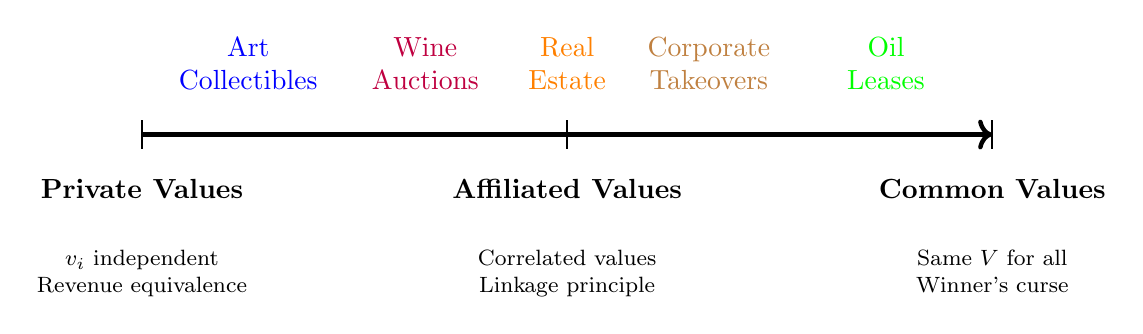
\begin{tikzpicture}[scale=0.9]
  % Main spectrum line
  \draw[ultra thick, ->] (0,0) -- (12,0);
  
  % Key points
  \draw[thick] (0,-0.2) -- (0,0.2);
  \draw[thick] (6,-0.2) -- (6,0.2);
  \draw[thick] (12,-0.2) -- (12,0.2);
  
  % Labels
  \node[below] at (0,-0.5) {\textbf{Private Values}};
  \node[below] at (6,-0.5) {\textbf{Affiliated Values}};
  \node[below] at (12,-0.5) {\textbf{Common Values}};
  
  % Examples with colors
  \node[above, blue, align=center] at (1.5,0.5) {Art\\Collectibles};
  \node[above, purple, align=center] at (4,0.5) {Wine\\Auctions};
  \node[above, orange, align=center] at (6,0.5) {Real\\Estate};
  \node[above, brown, align=center] at (8,0.5) {Corporate\\Takeovers};
  \node[above, green, align=center] at (10.5,0.5) {Oil\\Leases};
  
  % Characteristics
  \node[below, font=\footnotesize, align=center] at (0,-1.5) {$v_i$ independent\\Revenue equivalence};
  \node[below, font=\footnotesize, align=center] at (6,-1.5) {Correlated values\\Linkage principle};
  \node[below, font=\footnotesize, align=center] at (12,-1.5) {Same $V$ for all\\Winner's curse};
\end{tikzpicture}
\end{center}


\textbf{Mathematical Representation:}
$$v_i = \alpha \cdot \text{(private component)} + (1-\alpha) \cdot \text{(common component)}$$
where $\alpha \in [0,1]$ determines position on spectrum
\end{frame}

\begin{frame}{Affiliation: Formal Definition}
\textbf{Affiliated Random Variables:}
Variables $(X_1, ..., X_n)$ are affiliated if:
$$f(x \vee x') \cdot f(x \wedge x') \geq f(x) \cdot f(x')$$
where $\vee$ = component-wise max, $\wedge$ = component-wise min


\textbf{Intuition:}
\begin{itemize}
  \item Higher values of one variable make higher values of others more likely
  \item Positive correlation, but stronger
  \item Common in auction settings
\end{itemize}

\textbf{Examples:}
\begin{itemize}
  \item Signals about common value
  \item Expert evaluations of artwork
  \item Geological surveys for oil
\end{itemize}
\end{frame}

\begin{frame}{The Linkage Principle Visualized}
\begin{center}
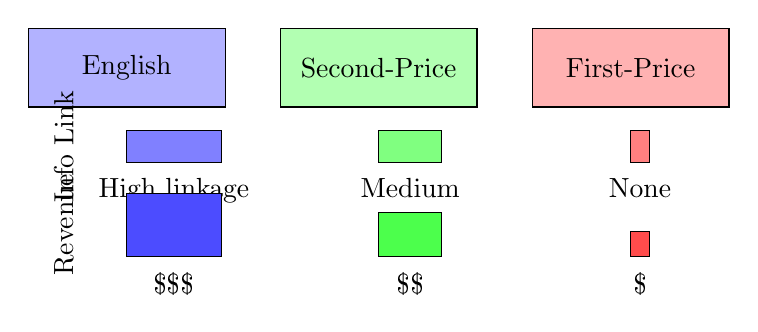
\begin{tikzpicture}[scale=0.8]
  % Auction formats
  \node[draw, rectangle, fill=blue!30, minimum width=2.5cm, minimum height=1cm] (eng) at (0,3) {English};
  \node[draw, rectangle, fill=green!30, minimum width=2.5cm, minimum height=1cm] (sp) at (4,3) {Second-Price};
  \node[draw, rectangle, fill=red!30, minimum width=2.5cm, minimum height=1cm] (fp) at (8,3) {First-Price};
  
  % Information linkage bars
  \draw[fill=blue!50] (0,1.5) rectangle (1.5,2);
  \draw[fill=green!50] (4,1.5) rectangle (5,2);
  \draw[fill=red!50] (8,1.5) rectangle (8.3,2);
  
  \node[below] at (0.75,1.4) {High linkage};
  \node[below] at (4.5,1.4) {Medium};
  \node[below] at (8.15,1.4) {None};
  
  % Revenue bars
  \draw[fill=blue!70] (0,0) rectangle (1.5,1);
  \draw[fill=green!70] (4,0) rectangle (5,0.7);
  \draw[fill=red!70] (8,0) rectangle (8.3,0.4);
  
  \node[below] at (0.75,-0.1) {\$\$\$};
  \node[below] at (4.5,-0.1) {\$\$};
  \node[below] at (8.15,-0.1) {\$};
  
  % Labels
  \node[rotate=90] at (-1,0.5) {Revenue};
  \node[rotate=90] at (-1,1.75) {Info Link};
\end{tikzpicture}
\end{center}

\textbf{Milgrom-Weber Revenue Ranking:}
$$\E[\text{Revenue}]_{\text{English}} \geq \E[\text{Revenue}]_{\text{Second-Price}} \geq \E[\text{Revenue}]_{\text{First-Price}}$$

\textbf{Key Insight:} Linking winner's payment to others' information reduces winner's information rent
\end{frame}

\begin{frame}{Linkage Principle: Policy Implications}
\textbf{Seller Should Reveal Information:}
\begin{itemize}
  \item Commit to honestly reveal all information
  \item Reduces winner's curse, more aggressive bidding
  \item Increases expected revenue
  \item Even if information is bad!
\end{itemize}


\textbf{Examples:}
\begin{itemize}
  \item Art: Provide authentication, condition reports
  \item Real estate: Home inspections, disclosures
  \item Oil rights: Share geological surveys
  \item Companies: Due diligence data rooms
\end{itemize}


\textbf{Reserve Price Policy:}
\begin{itemize}
  \item Public reserve better than secret reserve
  \item Provides information about seller's valuation
  \item Links payment to seller's information
\end{itemize}
\end{frame}

%===============================================
\subsection{Strategic Considerations}
%===============================================

\begin{frame}{The Wallet Game (Klemperer 1998)}
\textbf{Model ``Almost Common Values'':}
$$v_i = \alpha t_i + \beta \sum_{j \neq i} t_j$$

\begin{itemize}
  \item $\alpha = \beta$: Pure common value (sum of all signals)
  \item $\beta = 0$: Pure private value
  \item $\alpha > \beta$: Mostly private with common element
\end{itemize}


\textbf{English Auction Equilibrium:}
\begin{itemize}
  \item First dropout: $p_1 = (\alpha + (n-1)\beta)t_{(n)}$
  \item Information revealed at each dropout
  \item Final price: $p = \beta\sum_{j=3}^n t_{(j)} + (\alpha + \beta)t_{(2)}$
\end{itemize}

\textbf{Key Result:}
Small advantage ($\alpha$ slightly larger) creates large competitive advantage in English auction with common values
\end{frame}

\begin{frame}{Entry and Information Acquisition}
\begin{center}
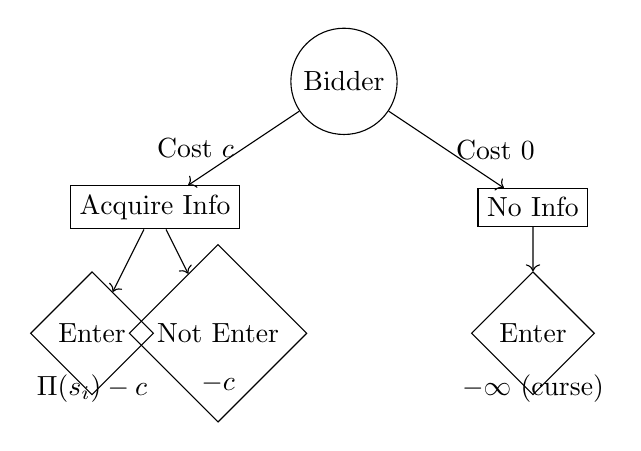
\begin{tikzpicture}[scale=0.8]
  % Decision tree
  \node[draw, circle] (start) at (0,0) {Bidder};
  \node[draw, rectangle] (acquire) at (-3,-2) {Acquire Info};
  \node[draw, rectangle] (noinfo) at (3,-2) {No Info};
  
  \draw[->] (start) -- (acquire) node[midway,left] {Cost $c$};
  \draw[->] (start) -- (noinfo) node[midway,right] {Cost $0$};
  
  \node[draw, diamond] (enter1) at (-4,-4) {Enter};
  \node[draw, diamond] (nenter1) at (-2,-4) {Not Enter};
  \node[draw, diamond] (enter2) at (3,-4) {Enter};
  
  \draw[->] (acquire) -- (enter1);
  \draw[->] (acquire) -- (nenter1);
  \draw[->] (noinfo) -- (enter2);
  
  % Payoffs
  \node[below] at (-4,-4.5) {$\Pi(s_i) - c$};
  \node[below] at (-2,-4.5) {$-c$};
  \node[below] at (3,-4.5) {$-\infty$ (curse)};
\end{tikzpicture}
\end{center}

\textbf{Equilibrium Effects:}
\begin{itemize}
  \item Information acquisition creates entry barrier
  \item Uninformed bidders face severe winner's curse
  \item Can lead to thin markets or market breakdown
  \item English auctions partially mitigate through revelation
\end{itemize}
\end{frame}

%===============================================
\subsection{Summary and Key Takeaways}
%===============================================

\begin{frame}{Summary: Core Concepts}
\begin{enumerate}
  \item \textbf{Winner's Curse}
  \begin{itemize}
    \item Arises in common value settings
    \item Winning is ``bad news'' about value
    \item Rational bidders must shade bids accordingly
  \end{itemize}
  
  \item \textbf{Information Revelation}
  \begin{itemize}
    \item English auctions reveal information progressively
    \item Reduces uncertainty and winner's curse
    \item Enables more aggressive bidding
  \end{itemize}
  
  \item \textbf{Linkage Principle}
  \begin{itemize}
    \item Link payment to others' information
    \item Reduces information rents
    \item English $\geq$ Second-Price $\geq$ First-Price
  \end{itemize}
  
  \item \textbf{Affiliation}
  \begin{itemize}
    \item Stronger than correlation
    \item Common in real auctions
    \item Breaks revenue equivalence
  \end{itemize}
\end{enumerate}
\end{frame}

\begin{frame}{Key Takeaways for Practice}
\begin{tcolorbox}[colback=blue!5!white,colframe=blue!75!black,title=For Sellers]
\begin{itemize}
  \item Use English auctions when values are affiliated/common
  \item Commit to reveal all information (even bad news)
  \item Set public rather than secret reserve prices
  \item Provide inspection opportunities and documentation
\end{itemize}
\end{tcolorbox}

\begin{tcolorbox}[colback=green!5!white,colframe=green!75!black,title=For Bidders]
\begin{itemize}
  \item Account for winner's curse in common value settings
  \item Bid more conservatively with more competitors
  \item Value information acquisition opportunities
  \item Update beliefs in ascending auctions
\end{itemize}
\end{tcolorbox}

\begin{tcolorbox}[colback=red!5!white,colframe=red!75!black,title=For Mechanism Designers]
\begin{itemize}
  \item Consider information structure when choosing format
  \item Design for appropriate information revelation
  \item Account for entry and information acquisition incentives
\end{itemize}
\end{tcolorbox}
\end{frame}

\begin{frame}{Mathematical Summary}
\textbf{Key Equilibrium Conditions:}

\begin{block}{Common Value Second-Price}
$$b(s_i) = \E[V | S_i = s_i, S_{(n-1)} = s_i]$$
\end{block}

\begin{block}{Revenue Ranking with Affiliation}
$$R_{English} = \E[v_{(2)}(S_{(2)}, S_{(2)}, S_{(3)}, ..., S_{(n)})]$$
$$R_{Second} = \E[v_{(2)}(S_{(2)}, S_{(2)}, S_{(2)}, ..., S_{(2)})]$$
$$R_{First} = \E[v_{(2)}(S_{(2)}, S_{(1)}, S_{(1)}, ..., S_{(1)})]$$
\end{block}

\begin{block}{Linkage Principle}
Higher correlation between payment and others' signals $\Rightarrow$ Higher expected revenue
\end{block}
\end{frame}

\part{Extensions}

\section{Multi Unit}

\begin{frame}{Multi-Unit Auctions}
\textbf{Setting:} $k$ identical units, $n$ bidders, each wants one unit

\textbf{Uniform Price Auction:}
\begin{itemize}
  \item All winners pay same price (e.g., $(k+1)$-th highest bid)
  \item Strategic: Demand reduction incentive
  \item Used in Treasury bill auctions
\end{itemize}

\textbf{Discriminatory (Pay-as-bid) Auction:}
\begin{itemize}
  \item Each winner pays own bid
  \item Similar to first-price auction analysis
  \item Also used in some Treasury auctions
\end{itemize}

\textbf{Vickrey-Clarke-Groves (VCG):}
\begin{itemize}
  \item Generalization of second-price auction
  \item Each pays externality imposed on others
  \item Efficient but complex, rarely used
\end{itemize}
\end{frame}



\begin{frame}{Multi-Unit Auction Formats}
\textbf{Setting:} $K$ identical units, $n$ bidders, each wants multiple units


\textbf{1. Discriminatory (Pay-as-Bid) Auction:}
\begin{itemize}
  \item Submit bid schedule $(q_i, b_i(q))$ for quantities
  \item Winners pay own bids for units won
  \item Strategic bid shading on all units
  \item Used in some Treasury bill auctions
\end{itemize}

\textbf{2. Uniform Price Auction:}
\begin{itemize}
  \item All winners pay same market-clearing price
  \item Price = highest rejected bid or lowest accepted
  \item Demand reduction problem (strategic underbidding)
  \item Used in electricity markets, IPOs
\end{itemize}

\textbf{3. Vickrey (Generalized Second-Price):}
\begin{itemize}
  \item Each pays opportunity cost imposed on others
  \item Truthful bidding is dominant strategy
  \item Complex to understand and implement
  \item Rarely used in practice
\end{itemize}
\end{frame}

\begin{frame}{Demand Reduction Problem}
\textbf{Issue in Uniform Price Auctions:}

Bidding on marginal unit affects price for ALL units won


\textbf{Example:} 2 units available, 2 bidders
\begin{itemize}
  \item Bidder 1 values: $v_{11} = 10, v_{12} = 8$
  \item Bidder 2 values: $v_{21} = 9, v_{22} = 7$
  \item Efficient: Each gets one unit
\end{itemize}

\textbf{But in equilibrium:}
\begin{itemize}
  \item Bidder 2 may bid: $b_{21} = 9, b_{22} < 7$
  \item Reduces demand to lower price on first unit
  \item Bidder 1 might win both units (inefficient!)
\end{itemize}

\textbf{Consequences:}
\begin{itemize}
  \item Inefficient allocation
  \item Lower revenue than discriminatory auction possible
  \item Facilitates collusion
\end{itemize}
\end{frame}

\begin{frame}{Vickrey Auction for Multiple Units}
\textbf{Payment Rule:}
Bidder $i$ pays the externality imposed on others:
$p_i = \sum_{j \neq i} v_j(\text{allocation without } i) - \sum_{j \neq i} v_j(\text{allocation with } i)$


\textbf{Example:} 2 units, 3 bidders with unit demands
\begin{itemize}
  \item Values: $v_1 = 10, v_2 = 8, v_3 = 6$
  \item Allocation: Bidders 1 and 2 win
  \item Bidder 1 pays: $6$ (displaces bidder 3)
  \item Bidder 2 pays: $6$ (displaces bidder 3)
  \item Bidder 3 pays: $0$
\end{itemize}

\textbf{Properties:}
\begin{itemize}
  \item Dominant strategy: Report true values
  \item Efficient allocation
  \item But: Complex, low revenue possible, not collusion-proof
\end{itemize}
\end{frame}

%===============================================
\section{Summary and Key Takeaways}
%===============================================

\begin{frame}{Summary: Core Results}
\textbf{1. Equilibrium Strategies:}
\begin{itemize}
  \item English/Vickrey: Bid true value (dominant strategy)
  \item First-Price/Dutch: Shade bid below value
  \item Shading depends on competition and distribution
\end{itemize}

\textbf{2. Revenue Equivalence (IPV, risk-neutral, symmetric):}
\begin{itemize}
  \item All standard formats yield same expected revenue
  \item Revenue = $\E[v_{(2)}]$ (expected second-highest value)
  \item Breaks with risk aversion, asymmetry, or correlation
\end{itemize}

\textbf{3. Optimal Design:}
\begin{itemize}
  \item Reserve price improves revenue
  \item Virtual valuation determines optimal allocation
  \item Standard auction + reserve achieves optimum
\end{itemize}
\end{frame}




\begin{frame}{Key Insights for Practice}
\textbf{Choosing an Auction Format:}

\begin{tabular}{ll}
\toprule
\textbf{Use English/Ascending when:} & \textbf{Use Sealed-Bid when:} \\
\midrule
Common value elements & Preventing collusion important \\
Want price discovery & Speed matters \\
Affiliation present & Bidders geographically dispersed \\
Transparency important & Privacy concerns \\
\bottomrule
\end{tabular}


\textbf{Design Recommendations:}
\begin{itemize}
  \item Always set optimal reserve price
  \item Reveal information to reduce winner's curse
  \item First-price better with risk-averse bidders
  \item Consider entry fees and participation costs
  \item Multi-unit: Be aware of demand reduction
\end{itemize}

\textbf{Remember:} Real auctions rarely satisfy all RET assumptions!
\end{frame}

%%%%%%%%%%%%%%%%%%%%%%%%%%%%


%================================================
\section{Multi-Unit and Combinatorial Auctions}
%================================================

\begin{frame}{Multi-Unit Auctions: Beyond Single Items}
\textbf{Types of Multi-Unit Auctions:}
\begin{itemize}
  \item \textbf{Uniform Price:} All winners pay the same market-clearing price
  \item \textbf{Discriminatory (Pay-as-Bid):} Each winner pays their own bid
  \item \textbf{Vickrey-Clarke-Groves (VCG):} Generalized second-price mechanism
\end{itemize}


\textbf{Key Design Challenges:}
\begin{enumerate}
  \item \textbf{Demand Reduction:} Strategic underbidding on marginal units
  \item \textbf{Market Power:} Large bidders can manipulate clearing price
  \item \textbf{Efficiency vs Revenue:} Trade-off becomes more complex
\end{enumerate}


\begin{tcolorbox}[colback=blue!5!white,colframe=blue!75!black,title=Treasury Auction Example]
US Treasury uses discriminatory format for bills, uniform price for notes/bonds. 
Annual volume: \$12+ trillion (2023)
\end{tcolorbox}
\end{frame}

\begin{frame}{Combinatorial Auctions: Package Bidding}
\textbf{The Combinatorial Allocation Problem (CAP):}
\begin{align}
\max_{x_{iS}} & \sum_{i \in N} \sum_{S \subseteq M} v_{iS} x_{iS} \\
\text{s.t. } & \sum_{S: j \in S} \sum_{i \in N} x_{iS} \leq 1, \quad \forall j \in M \\
& \sum_{S \subseteq M} x_{iS} \leq 1, \quad \forall i \in N \\
& x_{iS} \in \{0,1\}
\end{align}

\textbf{Complexity and Bidding Languages:}
\begin{itemize}
  \item \textbf{XOR Bids:} ``A OR B but not both'' - Mutually exclusive packages
  \item \textbf{OR Bids:} ``A AND/OR B'' - Any combination acceptable
  \item \textbf{OR-of-XORs:} Nested structure for complex preferences
\end{itemize}

\textbf{Real-World Applications:}
\begin{itemize}
  \item Spectrum auctions (FCC, Ofcom): \$100+ billion raised
  \item Procurement (Chile school meals): 20\% cost reduction
  \item Transportation (logistics): Route optimization
\end{itemize}
\end{frame}


\part{Relaxing assumptions}
%===============================================
\section{Relaxing the Assumptions}
%===============================================

\begin{frame}{Assumptions for Revenue Equivalence}
\begin{enumerate}
    \item \textbf{Risk Neutrality} Bidders maximize expected surplus (not risk-averse)
    
    \item \textbf{Independent Private Values (IPV)} Each bidder knows their own valuation $v_i$, but valuations are drawn independently from distributions
    
    \item \textbf{Symmetry} All bidders draw valuations from the same distribution $F(v)$
    
    \item \textbf{Allocation Efficiency} The bidder with the highest valuation wins. 
    
    \item \textbf{Losers Pay Zero} Bidders who don't win pay nothing
    
    \item \textbf{Boundary Condition} Expected payment is zero when valuation is zero $E[\text{payment} \mid v_i = 0] = 0$
\end{enumerate}

\textbf{Key insight} Any auction mechanism satisfying these assumptions yields the same expected revenue.
\end{frame}

\subsection{Relaxing risk neutrality}

\begin{frame}{Relaxing Risk Neutrality}
\textbf{The Assumption:} Bidders maximize expected monetary value (risk-neutral)


\textbf{Reality:} Most bidders are risk-averse
\begin{itemize}
  \item Prefer certain \$50 over 50\% chance of \$100
  \item Utility function $U(x)$ is concave: $U''(x) < 0$
  \item Common measures: constant relative risk aversion (CRRA), constant absolute risk aversion (CARA)
\end{itemize}

\textbf{Impact on Standard Formats:}
\begin{itemize}
  \item \textbf{English \& Second-Price:} \textcolor{green!70!black}{No impact!}
  \begin{itemize}
    \item Bidding true value still dominant strategy
    \item Risk preferences don't affect optimal bid
    \item Revenue unchanged
  \end{itemize}
  
  \item \textbf{First-Price \& Dutch:} \textcolor{orange}{Higher bids!}
  \begin{itemize}
    \item Risk-averse bidders bid \textit{closer to true value}
    \item Trade-off: Lower win probability vs. avoiding risk of not winning
    \item \textbf{Higher revenue for seller}
    \item Efficiency still preserved (highest value still wins)
  \end{itemize}
\end{itemize}
\end{frame}

\begin{frame}{Risk Aversion in First-Price Auctions: Why Bid Higher?}
\textbf{Intuition:} Risk-averse bidders dislike uncertainty

\begin{center}
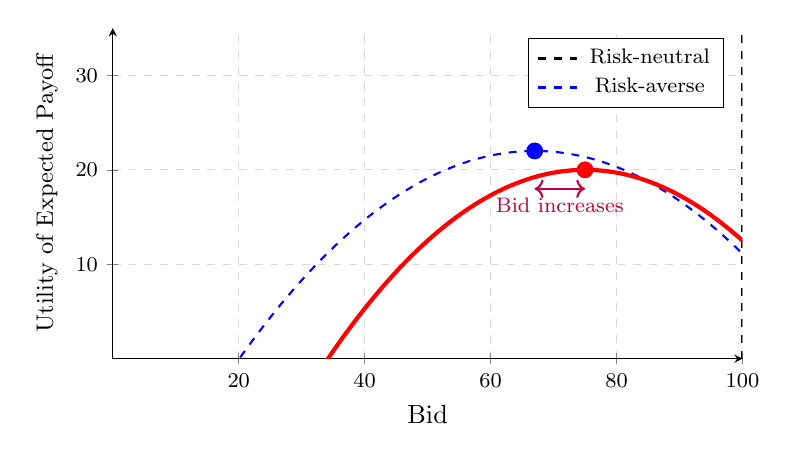
\begin{tikzpicture}[scale=0.95]
  \begin{axis}[
    xlabel={Bid},
    ylabel={Utility of Expected Payoff},
    xmin=0, xmax=100,
    ymin=0, ymax=35,
    axis lines=middle,
    width=10cm,
    height=6cm,
    grid=major,
    grid style={dashed, gray!30},
    xtick={0,20,40,60,80,100},
    ytick={0,10,20,30},
    xlabel style={font=\small},
    xlabel near ticks, 
    ylabel near ticks, 
    ylabel style={font=\small},
    tick label style={font=\footnotesize},
    legend pos=north east,
    legend style={font=\footnotesize}
  ]
  
  % True value line
  \addplot[domain=0:100, samples=2, very thick, black, dashed] coordinates {(100,0) (100,35)};
  \node[font=\footnotesize] at (axis cs:100,37) {Your Value \$100K};
  
  % Risk-neutral expected utility curve
  \addplot[domain=0:100, samples=100, thick, blue, dashed] {-0.01*(x-67)^2 + 22};
  \addlegendentry{Risk-neutral}
  
  % Risk-averse expected utility curve (peaks earlier, lower)
  \addplot[domain=0:100, samples=100, ultra thick, red] {-0.012*(x-75)^2 + 20};
  \addlegendentry{Risk-averse}
  
  % Optimal bid markers
  \addplot[mark=*, mark size=3pt, only marks, blue] coordinates {(67,22)};
  \addplot[mark=*, mark size=3pt, only marks, red] coordinates {(75,20)};
  
  % Arrows showing shift
  \draw[<->, thick, purple] (axis cs:67,18) -- (axis cs:75,18);
  \node[below, purple, font=\footnotesize] at (axis cs:71,18) {Bid increases};
  
  \end{axis}
\end{tikzpicture}
\end{center}

\textbf{Key Insight:} Risk aversion shifts optimal bid higher because:
\begin{itemize}
  \item Risk-averse bidder values \textit{certainty} of winning
  \item Willing to sacrifice some profit to increase win probability
  \item Acts as "competition substitute" - higher bids even with same number of bidders
\end{itemize}
\end{frame}

\begin{frame}{Risk Aversion: Revenue Rankings Change}
\textbf{Revenue Equivalence Breaks Down!}


\textbf{With Risk-Neutral Bidders:}
\begin{center}
First-Price Revenue = Second-Price Revenue = English Revenue
\end{center}


\textbf{With Risk-Averse Bidders:}
\begin{center}
\textcolor{red}{\textbf{First-Price Revenue $>$ Second-Price Revenue = English Revenue}}
\end{center}


\textbf{Why This Happens:}
\begin{itemize}
  \item In second-price/English: Bidding true value still optimal 
  \item In first-price: Risk aversion increases bids above risk-neutral level
  \item \textbf{Practical implication:} Sellers benefit from first-price when bidders are risk-averse
\end{itemize}


\textbf{Efficiency:}
\begin{itemize}
  \item \textcolor{green!70!black}{\textbf{Preserved in all formats!}}
  \item Highest-value bidder still wins (just pays more in first-price)
\end{itemize}
\end{frame}

\begin{frame}{All-Pay Auctions with Risk Aversion}
\textbf{The Dangerous Combination:} Risk aversion + pay even if you lose

\textbf{Strategic Effects:}
\begin{itemize}
  \item Risk-averse bidders \textit{extremely} conservative in all-pay auctions
  \item Two sources of risk:
  \begin{enumerate}
    \item Risk of losing and paying your bid (standard all-pay risk)
    \item Risk aversion amplifies the pain of losing
  \end{enumerate}
  \item \textbf{Result:} Much lower bids than risk-neutral all-pay auction
  \item \textbf{Revenue:} Dramatically lower for seller
\end{itemize}


\begin{center}
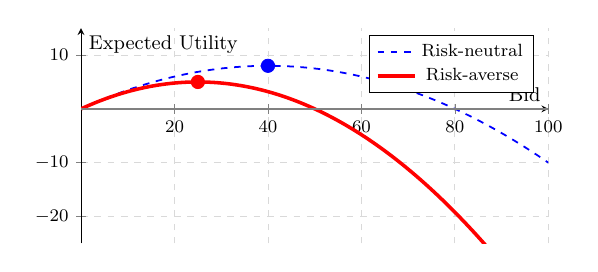
\begin{tikzpicture}[scale=0.8]
  \begin{axis}[
    xlabel={Bid},
    ylabel={Expected Utility},
    xmin=0, xmax=100,
    ymin=-25, ymax=15,
    axis lines=middle,
    width=9cm,
    height=5cm,
    grid=major,
    grid style={dashed, gray!30},
    xtick={0,20,40,60,80,100},
    ytick={-20,-10,0,10},
    xlabel style={font=\small},
    ylabel style={font=\small},
    tick label style={font=\footnotesize},
    legend pos=north east,
    legend style={font=\footnotesize}
  ]
  
  % Risk-neutral curve (from earlier slide)
  \addplot[domain=0:100, samples=100, thick, blue, dashed] {-0.005*(x-40)^2 + 8};
  \addlegendentry{Risk-neutral}
  
  % Risk-averse curve (peaks much earlier and lower)
  \addplot[domain=0:100, samples=100, ultra thick, red] {-0.008*(x-25)^2 + 5};
  \addlegendentry{Risk-averse}
  
  % Optimal bid markers
  \addplot[mark=*, mark size=3pt, only marks, blue] coordinates {(40,8)};
  \addplot[mark=*, mark size=3pt, only marks, red] coordinates {(25,5)};
  
  % Zero line
  \addplot[domain=0:100, samples=2, thick, gray] coordinates {(0,0) (100,0)};
  
  \end{axis}
\end{tikzpicture}
\end{center}

\textit{Risk aversion + all-pay = very low bidding and participation}
\end{frame}

\subsection{Asymmetric Bidders}
%===============================================
\begin{frame}{Relaxing Symmetry}
\textbf{The Assumption:} All bidders draw values from the same distribution $F(v)$


\textbf{Reality:} Different bidder types (strong vs. weak, informed vs. uninformed)
\begin{itemize}
  \item Strong bidders: Values from $F_S(v)$ with higher support
  \item Weak bidders: Values from $F_W(v)$ with lower support
\end{itemize}


\textbf{Impact on Standard Formats:}
\begin{itemize}
  \item \textbf{English \& Second-Price:} \textcolor{green!70!black}{No impact!}
  \begin{itemize}
    \item Still dominant strategy to bid true value
    \item Efficient allocation preserved
    \item Revenue = second-highest value
  \end{itemize}
  
  \item \textbf{First-Price \& Dutch:} \textcolor{red}{Major changes!}
  \begin{itemize}
    \item Different equilibrium bid functions $B_i(v)$ per type
    \item \textbf{Efficiency may be lost}: Weak bidder with higher value may lose to strong bidder with lower value
    \item Revenue effects ambiguous (could increase or decrease)
  \end{itemize}
\end{itemize}
\end{frame}

\begin{frame}{Asymmetric Bidders: Setup}
\textbf{Relaxing Symmetry Assumption:}
\begin{itemize}
  \item Different types of bidders
  \item Type $i$ values drawn from $F_i(v)$
  \item Each knows own type and others' types
  \item But not actual realizations
\end{itemize}


\textbf{English \& Vickrey:} No change!
\begin{itemize}
  \item Still dominant strategy to bid value
  \item Efficient allocation (highest value wins)
  \item Revenue = second-highest value
\end{itemize}


\textbf{First-Price \& Dutch:} Major changes!
\begin{itemize}
  \item Different equilibrium bid functions $B_i(v)$
  \item May be inefficient: $v_a > v_b$ but $B_i(v_a) < B_j(v_b)$ possible
  \item No general revenue ranking vs. second-price
  \item Complex equilibrium computation
\end{itemize}
\end{frame}

\begin{frame}{Visualization: Asymmetric Equilibrium}
\begin{center}
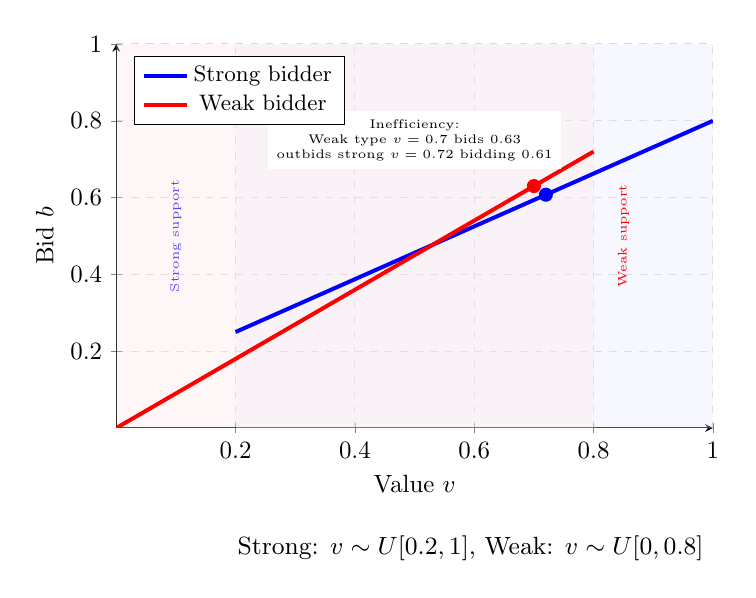
\begin{tikzpicture}[scale=0.9]
  \begin{axis}[
    xlabel={Value $v$},
    ylabel={Bid $b$},
    xmin=0, xmax=1,
    ymin=0, ymax=1,
    axis lines=middle,
    legend pos=north west,
    legend style={font=\small},
    xlabel near ticks, 
    ylabel near ticks, 
    width=10cm,
    height=7cm,
    grid=major,
    grid style={dashed, gray!30}
  ]
  
  % Strong bidder distribution support [0.2, 1]
  \fill[blue!10, opacity=0.3] (axis cs:0.2,0) rectangle (axis cs:1,1);
  \node[blue, rotate=90] at (axis cs:0.1,0.5) {\tiny Strong support};
  
  % Weak bidder distribution support [0, 0.8]
  \fill[red!10, opacity=0.3] (axis cs:0,0) rectangle (axis cs:0.8,1);
  \node[red, rotate=90] at (axis cs:0.85,0.5) {\tiny Weak support};
  
  % Strong bidder bid function: approximately linear from (0.2, 0.25) to (1, 0.8)
  \addplot[domain=0.2:1, ultra thick, blue] {0.6875*x + 0.1125};
  \addlegendentry{Strong bidder}
  
  % Weak bidder bid function: approximately linear from (0, 0) to (0.8, 0.72)
  \addplot[domain=0:0.8, ultra thick, red] {0.9*x};
  \addlegendentry{Weak bidder}
  
  % Inefficiency region: where weak bidder with lower value outbids strong bidder
  % Weak with v=0.7 bids 0.63, strong with v=0.72 bids 0.6075
  % \draw[thick, dashed, purple] (axis cs:0.7,0) -- (axis cs:0.7,0.63);
  % \draw[thick, dashed, purple] (axis cs:0.72,0) -- (axis cs:0.72,0.6075);
  
  \node[circle, fill=red, inner sep=2pt] at (axis cs:0.7,0.63) {};
  \node[circle, fill=blue, inner sep=2pt] at (axis cs:0.72,0.6075) {};
  
  % \draw[<->, thick, purple] (axis cs:0.7,0.63) -- (axis cs:0.72,0.6075);
  
  % Annotation for inefficiency
  \node[align=center, font=\tiny, fill=white] at (axis cs:0.5,0.75) {
    Inefficiency:\\
    Weak type $v=0.7$ bids $0.63$\\
    outbids strong $v=0.72$ bidding $0.61$
  };
  
  \end{axis}
  \node[align=center] at (5,-1.7) {\small Strong: $v \sim U[0.2,1]$, Weak: $v \sim U[0,0.8]$};
\end{tikzpicture}
\end{center}
\end{frame}

\subsection{Relaxing Independent Private Values}

\begin{frame}{Relaxing Independent Private Values (IPV)}
\textbf{The Assumption:} Each bidder's value $v_i$ is independent of others' values


\textbf{Reality:} Common Value or Affiliated Value situations
\begin{itemize}
  \item \textbf{Common Values:} True value is the same for all bidders, but each has different information/signal
  \begin{itemize}
    \item Examples: Oil drilling rights, company acquisitions
  \end{itemize}
  \item \textbf{Affiliated Values:} Values are correlated (if one bidder has high value, likely others do too)
  \begin{itemize}
    \item Examples: Art, real estate with investment value
  \end{itemize}
\end{itemize}


\textbf{Key Problem: The Winner's Curse}
\begin{itemize}
  \item In common value auctions, winning often means you overestimated the value
  \item Rational bidders bid below their signal to avoid overpaying
  \item More severe in sealed-bid formats vs. ascending auctions
\end{itemize}
\end{frame}

\begin{frame}{Winner's Curse: The Danger of Common Values}
\textbf{Scenario:} Oil drilling rights with unknown reserves

\begin{center}
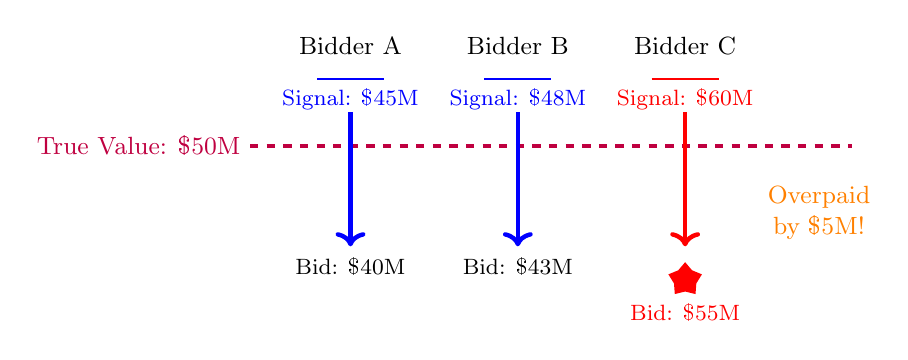
\begin{tikzpicture}[scale=0.85]
  % True value line
  \draw[ultra thick, dashed, purple] (0,2.5) -- (9,2.5);
  \node[left, purple, font=\small] at (0,2.5) {True Value: \$50M};
  
  % Bidders with their estimates
  \node[font=\small] at (1.5,4) {Bidder A};
  \node[font=\small] at (4,4) {Bidder B};
  \node[font=\small] at (6.5,4) {Bidder C};
  
  % Signal distributions
  \draw[thick, blue] (1,3.5) -- (2,3.5);
  \node[font=\footnotesize, blue] at (1.5,3.2) {Signal: \$45M};
  
  \draw[thick, blue] (3.5,3.5) -- (4.5,3.5);
  \node[font=\footnotesize, blue] at (4,3.2) {Signal: \$48M};
  
  \draw[thick, red] (6,3.5) -- (7,3.5);
  \node[font=\footnotesize, red] at (6.5,3.2) {Signal: \$60M};
  
  % Bids
  \draw[->, ultra thick, blue] (1.5,3) -- (1.5,1);
  \node[font=\footnotesize] at (1.5,0.7) {Bid: \$40M};
  
  \draw[->, ultra thick, blue] (4,3) -- (4,1);
  \node[font=\footnotesize] at (4,0.7) {Bid: \$43M};
  
  \draw[->, ultra thick, red] (6.5,3) -- (6.5,1);
  \node[font=\footnotesize, red] at (6.5,0) {Bid: \$55M};
  \node[star, star points=5, fill=red, inner sep=3pt] at (6.5,0.5) {};
  
  % Winner's curse annotation
  \node[orange, font=\small, align=center] at (8.5,1.5) {Overpaid\\by \$5M!};
\end{tikzpicture}
\end{center}

\textbf{Lesson:} C had the most optimistic (and wrong) signal and won, but overpaid
\end{frame}

\begin{frame}{Impact on Auction Formats: Common Values}
\textbf{English (Ascending) Auction:}
\begin{itemize}
  \item \textcolor{green!70!black}{\textbf{Advantage:}} Information revelation as bidders drop out
  \item Bidders update beliefs based on others' dropout prices
  \item Reduces winner's curse severity
  \item More efficient information aggregation
\end{itemize}


\textbf{Sealed-Bid Formats:}
\begin{itemize}
  \item \textcolor{red}{\textbf{Disadvantage:}} No information revelation
  \item Winner's curse is more severe
  \item Bidders shade bids more aggressively
  \item Lower revenue for seller
  \item \textbf{First-price better than second-price} (paradoxically)
\end{itemize}


\textbf{Key Result:} Revenue equivalence breaks down!
\begin{itemize}
  \item English $>$ First-Price $>$ Second-Price (typically)
\end{itemize}
\end{frame}

\begin{frame}{All-Pay Auctions with Common Values}
\textbf{The Brutal Combination:} Winner's curse + everyone pays


\textbf{Strategic Effects:}
\begin{itemize}
  \item Bidders must be even more conservative
  \item Risk of overpaying \textit{and} losing money even if you lose
  \item Very low equilibrium bids
  \item High variance in outcomes
\end{itemize}


\textbf{Real-World Examples:}
\begin{itemize}
  \item \textbf{R\&D races with uncertain market value}
  \begin{itemize}
    \item All firms invest (pay), winner gets patent
    \item Market value of patent uncertain (common value)
    \item Winner often finds market smaller than expected
  \end{itemize}
  \item \textbf{Lobbying for uncertain benefits}
  \begin{itemize}
    \item All parties spend on lobbying (all pay)
    \item Actual benefit of winning uncertain
  \end{itemize}
\end{itemize}

\vspace{0.2cm}
\textit{Moral: All-pay + common values = extremely conservative bidding}
\end{frame}

\subsection{Relaxing Other Key Assumptions}

\begin{frame}{Relaxing: More than one relaxation}
\textbf{The Assumption:} Only the winner pays; losers pay nothing

\textbf{Effects When Combined with Other Relaxations:}

\textbf{All-Pay + Risk Aversion:}
\begin{itemize}
  \item Extremely conservative bidding (compounding effect)
  \item Much lower revenue than standard auctions
  \item High-value bidders may not participate
\end{itemize}

\vspace{0.2cm}
\textbf{All-Pay + Asymmetric Bidders:}
\begin{itemize}
  \item Weak bidders bid even more conservatively
  \item Strong bidders can bid slightly more aggressively
  \item Winner selection may be inefficient
  \item No general formula for equilibrium
\end{itemize}
\end{frame}

\begin{frame}{Relaxing: Entry Costs and Participation}
\textbf{The Assumption:} Free entry, all interested bidders can participate


\textbf{Reality:} Entry costs, qualification requirements, participation barriers
\begin{itemize}
  \item Qualification fees or deposits
  \item Information acquisition costs
  \item Time and effort to prepare bids
\end{itemize}


\textbf{Impact on All Formats:}
\begin{itemize}
  \item \textbf{Fewer bidders participate}
  \begin{itemize}
    \item Lower competition $\rightarrow$ lower revenue
    \item Only high-value bidders enter
  \end{itemize}
  \item \textbf{Efficiency may improve or worsen}
  \begin{itemize}
    \item Better if entry costs filter out low-value bidders
    \item Worse if entry costs prevent high-value but resource-constrained bidders
  \end{itemize}
  \item \textbf{Seller trade-off:}
  \begin{itemize}
    \item High entry fees $\rightarrow$ fewer bidders but more serious competition
    \item Low entry fees $\rightarrow$ more bidders but potentially less serious
  \end{itemize}
\end{itemize}
\end{frame}

\begin{frame}{All-Pay Auctions with Entry Costs}
\textbf{The Compounding Effect:} Pay to enter + pay your bid regardless of outcome


\textbf{Strategic Implications:}
\begin{itemize}
  \item Extremely high barrier to participation
  \item Only bidders with very high expected values enter
  \item Very aggressive bidding among those who do enter (sunk cost of entry)
  \item Potential for very few participants
\end{itemize}


\textbf{Example: Patent Races with High R\&D Setup Costs}
\begin{itemize}
  \item Firms must invest in labs, hire researchers (entry cost)
  \item Then spend on actual R\&D (all-pay aspect)
  \item Winner gets patent, losers get nothing
  \item Result: Only 2-3 major firms compete in most drug categories
\end{itemize}


\textbf{Seller's Dilemma:}
\begin{itemize}
  \item Want enough bidders for competition
  \item But each bidder needs high expected surplus to cover entry + bidding costs
  \item Difficult to optimize
\end{itemize}
\end{frame}

\begin{frame}{Summary: Relaxing Assumptions \& All-Pay Formats}
\begin{center}
\begin{tabular}{|p{3cm}|p{3.5cm}|p{3cm}|}
\hline
\textbf{Relaxation} & \textbf{Standard Formats} & \textbf{All-Pay Formats} \\
\hline
\rowcolor{blue!10}
\textbf{Risk Aversion} & 
First-price: higher bids, same efficiency & 
Much more conservative bidding \\
\hline
\rowcolor{green!10}
\textbf{Asymmetry} & 
First-price: may lose efficiency & 
Weak bidders nearly don't bid \\
\hline
\rowcolor{yellow!10}
\textbf{Common Values} & 
English best; 1st $>$ 2nd price & 
Extremely low bids \\
\hline
\rowcolor{red!10}
\textbf{Entry Costs} & 
Fewer bidders, trade-off for seller & 
Very few bidders, high barrier \\
\hline
\end{tabular}
\end{center}

\vspace{0.4cm}
\textbf{Key Insight:} All-pay auctions are much more sensitive to assumption violations
\begin{itemize}
  \item Each violation compounds the "pay even if you lose" effect
  \item Results in very conservative bidding and low participation
  \item Use all-pay formats only when you truly need them (e.g., modeling contests, lobbying)
\end{itemize}
\end{frame}

\part{Applications}

%===============================================
\section{Real-World Applications}
%===============================================


\begin{frame}{Bloomberg Auction Mechanism – Key Features}

\textbf{Mechanism description (to be verified)}
\begin{itemize}
  \item A buyer (or seller) initiates an auction and selects a number of participating counterparties (“offerees”).
  \item Each offeree submits a bid (or offer) in the form of a buy-ask spread.
  \item The best (lowest cost) bid wins — i.e. the winner pays/submits their submitted price (first-price style).
  \item After the auction ends, the winner is informed of the second-best (runner‐up) bid.
\end{itemize}

\textbf{Applications}
\begin{itemize}
  \item Used in fixed-income or institutional trading environments where transparency and participation are controlled.
  \item The runner-up disclosure helps the winner gauge their pricing margin and negotiation leverage.
\end{itemize}

\textbf{Note} The precise implementation details (eligibility, bid format, timing, runner‐up disclosure) have **not** been fully verified via publicly accessible documentation.
\end{frame}


\begin{frame}{Online Marketplaces eBay vs. Amazon}
\begin{center}
\begin{tabular}{p{4.5cm}p{4.5cm}}
\toprule
\textbf{eBay Model} & \textbf{Amazon Model} \\
\midrule
\rowcolor{blue!10}
English auction format & Fixed price (Buy Now) \\
\rowcolor{green!10}
Time-limited bidding & Immediate purchase \\
\rowcolor{blue!10}
Price discovery & Price transparency \\
\rowcolor{green!10}
Seller sets reserve & Seller sets price \\
\rowcolor{blue!10}
Competition visible & Competition hidden \\
\rowcolor{green!10}
Good for unique items & Good for commodities \\
\bottomrule
\end{tabular}
\end{center}


\textbf{Trend} Even eBay now emphasizes "Buy It Now" for speed


\textbf{Lesson} Choose mechanism based on
\begin{itemize}
  \item Product uniqueness
  \item Buyer urgency
  \item Transaction costs
\end{itemize}
\end{frame}

%===============================================
\section{Procurement Applications}
%===============================================


\begin{frame}{Procurement Best Practices}
\textbf{Keys to Success}
\begin{itemize}
  \item \textbf{Qualify suppliers first} Don't sacrifice quality for price
  \item \textbf{Clear specifications} Avoid apples-to-oranges comparisons
  \item \textbf{Multiple rounds} Give suppliers chance to compete
  \item \textbf{Reserve your right} Don't have to accept lowest bid
\end{itemize}


\textbf{Common Mistakes}
\begin{itemize}
  \item Running auctions with only 2-3 suppliers
  \item Poorly defined requirements lead to disputes
  \item Focusing only on price, ignoring total cost
  \item Burning supplier relationships with aggressive tactics
\end{itemize}


\textbf{When to Avoid}
\begin{itemize}
  \item Strategic partnerships or highly customized products
  \item When you need innovation, not just low price
\end{itemize}
\end{frame}

%===============================================
\section{Marketplace Design}
%===============================================

\begin{frame}{Building a Marketplace Two-Sided Markets}
\textbf{Your Platform Connects Buyers and Sellers}

Examples eBay, Airbnb, Uber, AWS Spot Instances


\textbf{Key Challenges}
\begin{itemize}
  \item \textbf{Chicken-and-egg} Need both sides to participate
  \item \textbf{Pricing} Who pays? How much?
  \item \textbf{Quality and Trust} How to maintain standards?
\end{itemize}


\textbf{Auction Design Helps}
\begin{itemize}
  \item \textbf{Price discovery} Market finds the right price
  \item \textbf{Matching} Right buyers find right sellers
  \item \textbf{Efficiency} Resources go to highest value use
\end{itemize}


\textbf{Critical Decision} What's your objective?
\begin{itemize}
  \item Transaction volume? Revenue? Efficiency? Quality?
\end{itemize}
\end{frame}

\begin{frame}{Marketplace Design Strategic Choices}
\begin{center}
\begin{tabular}{|p{2.8cm}|p{2.8cm}|p{2.8cm}|}
\hline
\textbf{Choice} & \textbf{Option A} & \textbf{Option B} \\
\hline
\textbf{Pricing Model} & 
Commission on transactions &
Subscription/listing fees \\
\hline
\textbf{Competition} & 
Winner-take-all &
Multiple winners \\
\hline
\textbf{Transparency} & 
Show all bids/asks &
Hide competitor info \\
\hline
\textbf{Speed} & 
Real-time matching &
Batch at intervals \\
\hline
\textbf{Commitment} & 
Binding immediately &
Can cancel/modify \\
\hline
\end{tabular}
\end{center}


\textbf{eBay's Choices}
\begin{itemize}
  \item Second-price auctions for trust
  \item Reputation system for quality
  \item Buy-it-now for immediacy
\end{itemize}
\textit{Your design choices shape participant behavior}
\end{frame}

\part{Business applications}


%===============================================
\section{Business Frameworks \& Action Items}
%===============================================


\begin{frame}{Preventing Collusion}
\textbf{Collusion costs sellers billions annually}

\begin{center}
\begin{tabular}{p{4.5cm}p{4.5cm}}
\toprule
\textbf{Warning Signs} & \textbf{Countermeasures} \\
\midrule
\rowcolor{red!10}
Identical bids & Use sealed-bid formats \\
\rowcolor{red!10}
Rotating winners & Set meaningful reserves \\
\rowcolor{red!10}
Intentionally low bids & Limit information disclosure \\
\rowcolor{red!10}
Bid withdrawal patterns & Random participation rules \\
\rowcolor{red!10}
Few active bidders & Encourage new entrants \\
\bottomrule
\end{tabular}
\end{center}

\textbf{Best Practice}
\begin{itemize}
  \item Monitor bidding patterns over time
  \item Use sealed formats when collusion risk is high
  \item Keep reserve prices confidential
  \item Prosecute violations aggressively
\end{itemize}
\end{frame}

\begin{frame}{When Should You Use Auction Design?}
\textbf{Good Fit When}
\begin{itemize}
  \item Selling/buying scarce resources
  \item Value varies significantly across bidders
  \item You need price discovery
  \item You want competition to drive value
  \item You need transparent, defensible process
\end{itemize}


\textbf{Red Flags}
\begin{itemize}
  \item Few potential bidders (easier to collude)
  \item High complexity (hard to participate)
  \item Unclear valuation (creates uncertainty)
  \item High transaction costs
\end{itemize}
\end{frame}

\begin{frame}{Decision Framework 5 Key Questions}
\textbf{Before designing an auction, ask}
\begin{enumerate}
  \item \textbf{What are you selling?}
  \begin{itemize}
    \item Unique item $\rightarrow$ English auction
    \item Commodity $\rightarrow$ Sealed-bid
  \end{itemize}
  
  \item \textbf{Who are your bidders?}
  \begin{itemize}
    \item Few sophisticated $\rightarrow$ Watch for collusion
    \item Many casual $\rightarrow$ Keep it simple
  \end{itemize}
  
  \item \textbf{What's your goal?}
  \begin{itemize}
    \item Maximum revenue $\rightarrow$ Set optimal reserve
    \item Efficiency $\rightarrow$ English auction
  \end{itemize}
  
  \item \textbf{How much time do you have?}
  \begin{itemize}
    \item Days/weeks $\rightarrow$ English auction
    \item Minutes/hours $\rightarrow$ Sealed-bid
  \end{itemize}
  
  \item \textbf{What's your risk tolerance?}
  \begin{itemize}
    \item Risk-averse $\rightarrow$ Set higher reserve
    \item Risk-neutral $\rightarrow$ Optimize expected value
  \end{itemize}
\end{enumerate}
\end{frame}

\begin{frame}{Implementation Checklist}
\textbf{Before Launching}
\begin{enumerate}
  \item \textbf{Define Success Metrics}
  \begin{itemize}
    \item Revenue? Efficiency? Fairness? Speed?
  \end{itemize}
  
  \item \textbf{Know Your Participants}
  \begin{itemize}
    \item Sophistication level and collusion potential
  \end{itemize}
  
  \item \textbf{Set Clear Rules}
  \begin{itemize}
    \item Reserve prices, activity requirements, payment terms
  \end{itemize}
  
  \item \textbf{Plan for Edge Cases}
  \begin{itemize}
    \item What if no one bids? Everyone bids same? Manipulation?
  \end{itemize}
  
\end{enumerate}
\end{frame}

\begin{frame}{Red Flags When Market Design Is Failing}
\textbf{Warning Signs}
\begin{itemize}
  \item \textbf{Low participation} Only few bidders showing up
  \item \textbf{Unusual patterns} Everyone bids the same, or very high/low
  \item \textbf{Complaints} Participants say rules are unfair/unclear
  \item \textbf{Gaming} Evidence of manipulation or collusion
  \item \textbf{Instability} Prices swing wildly or predictably
  \item \textbf{Inefficiency} Wrong winners or resources misallocated
\end{itemize}


\textbf{What to Do}
\begin{itemize}
  \item Don't ignore the signals
  \item Gather data and analyze patterns
  \item Consult with participants
  \item Be willing to redesign
  \item Test changes carefully
\end{itemize}


\textit{California ignored warning signs for months before crisis hit}
\end{frame}

\begin{frame}{Quick Reference Best Practices}
\begin{center}
\begin{tcolorbox}[colback=green!5,colframe=green!40!black,title=DO]
\begin{itemize}
  \item Set a reserve price (almost always)
  \item Monitor for collusion patterns
  \item Keep rules simple and transparent
  \item Use sealed bids when collusion risk is high
\end{itemize}
\end{tcolorbox}

\begin{tcolorbox}[colback=red!5,colframe=red!40!black,title=DON'T]
\begin{itemize}
  \item Assume revenue equivalence always holds
  \item Reveal sensitive competitive information
  \item Use complex formats without expert help
  \item Ignore entry barriers and participation costs
\end{itemize}
\end{tcolorbox}
\end{center}
\end{frame}

\begin{frame}{Key Takeaways}
\textbf{The Big Ideas}

\begin{enumerate}
  \item \textbf{Design matters more than theory}
  \begin{itemize}
    \item Real-world context beats textbook solutions
  \end{itemize}
  
  \item \textbf{Auctions reveal private information}
  \begin{itemize}
    \item Better than posted prices when values uncertain
  \end{itemize}
  
  \item \textbf{Format choice depends on context}
  \begin{itemize}
    \item Under ideal conditions, all formats yield same revenue
    \item Choose based on practical considerations
  \end{itemize}
  
  \item \textbf{Real markets violate ideal conditions}
  \begin{itemize}
    \item Risk aversion, collusion, entry costs matter
    \item Anti-manipulation safeguards essential
  \end{itemize}
  
  \item \textbf{Simplicity beats sophistication}
  \begin{itemize}
    \item Participants must understand your mechanism
    \item Make honesty the dominant strategy
  \end{itemize}
\end{enumerate}
\end{frame}

\begin{frame}{Action Items}
\textbf{Immediate (This Week)}
\begin{itemize}
  \item Review your current procurement processes
  \item Identify opportunities for competitive bidding
\end{itemize}


\textbf{Short-term (This Month)}
\begin{itemize}
  \item Pilot a reverse auction for non-critical spend
  \item Benchmark against industry practices
  \item Train team on auction fundamentals
\end{itemize}


\textbf{Long-term (This Quarter)}
\begin{itemize}
  \item Assess platform/marketplace opportunities
  \item Develop auction strategy for key categories
  \item Build monitoring capabilities
\end{itemize}


\textbf{When to Bring in Experts}
\begin{itemize}
  \item High-stakes transactions (\$10M+)
  \item Complex multi-party negotiations
  \item New marketplace launches
  \item Signs of market manipulation
\end{itemize}
\end{frame}

\begin{frame}{Additional Resources}
\textbf{Want to learn more?}

\begin{itemize}
  \item \textbf{Books for Practitioners}
  \begin{itemize}
    \item "Auction Theory" by Vijay Krishna (intermediate)
    \item "Putting Auction Theory to Work" by Paul Milgrom (advanced)
  \end{itemize}
  
  \item \textbf{Industry Examples}
  \begin{itemize}
    \item FCC Spectrum Auctions (www.fcc.gov/auctions)
    \item Treasury Securities Auctions (www.treasurydirect.gov)
    \item Google Ads Help Center
  \end{itemize}
  
  \item \textbf{Expert Consultants}
  \begin{itemize}
    \item For high-stakes auctions (>\$1M), hire economists
    \item Firms NERA, Compass Lexecon, Analysis Group
  \end{itemize}
\end{itemize}


\begin{center}
\large Questions?
\end{center}
\end{frame}



\end{document}